% \documentstyle[a4,epic,eepic,epsf,titlepage,samplebox]{jreport}
\documentclass[a4,titlepage]{jsreport}

\usepackage[dvipdfmx]{graphicx}
\usepackage{fancyvrb}
\title{KLIC 講習会テキスト\\KL1 言語編}
\date{\ }
\author{平成5年12月~~財団法人 新世代コンピュータ技術開発機構~~作成
\\平成7年9月~~財団法人 日本情報処理開発協会開発研究室~~改訂}

\def\em{\bf\dg}
\let\dg\bf
% \newlength\miniwidth
% \newlength\boxoutmargin \boxoutmargin 3pt
% \newlength\boxinmargin \boxinmargin 10pt

\addtolength{\textheight}{27pt}
\addtolength{\topmargin}{-18pt}
\makeatletter
\let\savedchap\@makechapterhead
\def\@makechapterhead{\vspace*{-1cm}\savedchap}
\makeatletter

\newcounter{exercise}
\setcounter{exercise}{0}
\newcommand{\exercise}[1]{%
\section*{\refstepcounter{exercise}【演習問題\arabic{exercise}】 #1}}
\newcommand{\answer}[1]{%
\section*{\refstepcounter{exercise}【演習問題解答\arabic{exercise}】 #1}}

%\def\program{\begin{center}\miniwidth\columnwidth
%\advance\miniwidth-2\boxoutmargin
%\advance\miniwidth-2\boxinmargin
%\hbox\bgroup\hskip\boxoutmargin
%\vbox\bgroup\hrule\hbox\bgroup
%\vrule\hskip\boxinmargin\vbox\bgroup\vskip\boxinmargin\hbox\bgroup
%\begin{minipage}{\miniwidth}}
%\def\endprogram{\end{minipage}\egroup\vskip\boxinmargin\egroup
%\hskip\boxinmargin\vrule\egroup
%\hrule\egroup
%\hskip\boxoutmargin\egroup
%\end{center}}

\newenvironment{program}{\begin{quote}}{\end{quote}}

\tolerance 1000
\newcommand{\commit}{\texttt{|}}
% Makes underbar act like explicit hyphen
\def\_{\leavevmode \kern.06em \vbox{\hrule width.3em}\penalty\exhyphenpenalty}

\begin{document}
\maketitle

\chapter*{はじめに}

\bgroup\large
本編は KLIC 講習会のために作成した KL1 言語の入門テキストである.

KL1 言語について, まったくの白紙状態からの入門から, 若干複雑なプログラ
ムを組めるようになるための基本テクニックまでを解説した.

講習会テキストとしては, 別に「KLIC システム編」がある.  こちらは KLIC 
システムの具体的な使い方を解説したものである.  本編と合わせて御利用願
いたい.

種々のプログラム・テクニックの解説には演習問題を付け加えるようにした.
巻末に解答例を掲げたが, そこに与えた解答がベストとは限らない.  理解を
深め, また確認するために, これらの演習問題はぜひ自分で解いてみた上で, 
掲載した解答例と比較検討されることをお奨めしたい.

なお一部の内容は 1989 年に作成された新世代コンピュータ技術開発機構によ
る ''KL1 プログラミング入門編 / 初級編 / 中級編'' より引用した.

\begin{flushright}
1993年12月\\
ICOT KLIC 開発グループ\\
1995年9月\\
JIPDEC KLIC 保守普及グループ
\end{flushright}
\egroup
\thispagestyle{empty}

\newpage
\setcounter{page}{0}
\pagenumbering{roman}
\tableofcontents

\chapter{KL1 入門}
\setcounter{page}{0}
\pagestyle{plain}
\pagenumbering{arabic}

KL1 は並列論理型言語 Guarded Horn Clauses\cite{GHCoriginal} に基づいて
設計された, 並列処理の記述に適したプログラム言語で, 第五世代コンピュー
タプロジェクトがその目標としてきた並列推論システムの中核となる並列推論
マシンの共通核言語として, オペレーティング・システム\cite{PIMOS}から種々
の応用プログラムの記述にまで, 広く用いられてきた.\cite{KL-Design} この
章では KL1 の言語仕様の概略と, 基本的なプログラミング技法について解説
する.

\section{はじめに}

KL1 という言語の特徴をひとことで言うならば{\bf\dg 記号処理を並列に行な
うための言語}ということになる.

数値処理にくらべて記号処理では, 複雑に絡み合うデータを取り扱う必要があ
ることが多い.  このため, こうしたデータをどのようなデータ構造で表現す
るかが重要になる.  また, そうしたデータ構造をどのようにメモリ上 (ある
いはディスク装置上) で管理するかも問題である.  こうした管理にプログラ
マが多くの労力を割かずに済むように, 言語システムで基本的な機能を用意し
て, もっと本質的なプログラミングに集中できるようにしよう, というのが記
号処理言語の考え方である.  具体的には, 一意性のあるものに名前をつける
と自動的に一意な表現を与えてくれる{\em 記号アトム}の機構や, 標準的なデー
タ構造についてそのためのメモリ割り付けや解放の労力を減らしてくれる{\em 
自動メモリ管理}機構などが, 代表的な特徴である.  この点, KL1 は代表的な
記号処理言語である Lisp 一族と同様の機能を提供している.

並列処理のためには, 全体の処理を複数の部分処理に分割して, 必要なところ
では部分処理間の同期を取りながら計算を進める必要がある.  このために, 
逐次処理言語に並列実行を指定する機構と同期のための機構を追加し, 並列処
理にも使えるようにした言語 (あるいは OS の機能まで含めたシステム) は数
多い.

こうしたアプローチにはふたつの大きな問題点がある.  ひとつは, もともと
の言語の設計の原則は逐次処理のままなので, 並列に実行できる部分をいちい
ち指定しなければならないことである.  このため, 同じプログラムをプロセ
サ台数の大きく異なるハードウェアで共通に使い, しかも効率良く動かすよう
にすることが難しく, ハードウェアごとにプログラム全体をかなり書き直す必
要が生じる. まして, どのような並列処理が適当なのか良くわからない問題に
ついて, 実験を積み重ねながら並列処理の仕方を模索していくような場合, そ
のたびにプログラムを書き直してデバッグし直すことになり, 多大な労力が必
要になる.  もうひとつは同期処理の面倒さである.  同期の必要性を意識しな
がらのプログラミングは非常に厄介であるし, 同期にバグが入ると, そのバグ
がどのように表面化するかに再現性がない (実行するたびに違う現象が起きる) 
ことが多いので, デバッグは非常に困難になる.

KL1 は逐次処理に並列実行のための機構を付加するという方法で設計した言語
ではない.  最初からすべてが並行動作することを前提とした言語である.  こ
うすると非常に頻繁な同期が必要になるのだが, {\em データフロー同期機構}
を導入して同期を自動化することによって, プログラマによる同期の誤りが入
り込む可能性を排除している.  物理的な並列実行の指定は別途{\em プラグマ}
と呼ばれる記述によって行なう.  プラグマはプログラムの正当性
\footnote{正確には停止性を除いた部分正当性.}を変えないように設計してあ
るので, 並列処理の仕方を変えるたびにデバッグし直す必要がない.

こうした KL1 の特徴のおかげで, 並列処理ソフトウェアの研究開発の労力は
非常に軽減される.  同じプログラムのプラグマ部分を変更するだけでさまざ
まな並列実行の仕方を指定できるので, いったんバグを取ってしまえば並列実
行指定を変えるたびにバグに悩まされる必要はない.  このため第五世代コン
ピュータプロジェクトでは, 並列処理のもっとも困難な課題である負荷分散方
式の研究などを, 数多くの実験を行ないながら実証的に進めることができたわ
けである.

\section{構文と実行機構の基本}\label{outline}
まず KL1 のプログラム言語としての機構の概要を説明することにしよう.

\subsection{プログラムの形式と基本実行機構}
最初に KL1 のプログラムの形式と, 基本的な実行機構について, 簡単な例を
用いて解説する.

\subsubsection{簡単なプログラム}
もっとも簡単な KL1 プログラムの例として, 入力の 0, 1 を反転して出力す
るインバータを考えてみる.  プログラムは以下のように書ける.
\begin{program}
\begin{Verbatim}[baselinestretch=0.8]
not(In, Out):- In = 0 | Out = 1.
not(In, Out):- In = 1 | Out = 0.
\end{Verbatim}
\end{program}

この二行のプログラムは, それぞれ:
\begin{itemize}
\item
もし not の第一引数 In が 0 だったら, 第二引数 Out は 1 にする
\item
もし not の第一引数 In が 1 だったら, 第二引数 Out は 0 にする
\end{itemize}
と読む.  このふたつの行をそれぞれ{\em 節} (clause) と呼び, KL1 のプロ
グラムの基本単位である.

それぞれの節の冒頭部分にある ``{\tt not(In, Out)}'' は, この節が述語 
not に関する定義であること, 引数はふたつで, この節の中ではそれぞれ In,
Out と呼ぶことを宣言している.  この部分を節の{\em ヘッド} (head) と呼
ぶ.  {\em 述語}という名前は KL1 の論理型言語としての生い立ちから来るの
だが, ここでは単に手続き, あるいはサブルーチンのことだと思ってさしつか
えない.

ヘッドに続く ``{\tt :-}'' の後, 縦棒 (``\verb^|^'') の前までを{\em ガー
ド} (guard) と呼ぶ.  ガードはその節を選んで良いかどうかの条件を指定す
る条件部である.

縦棒の後, フルストップ (``{\tt .}'') までを{\em ボディ} (body) と呼ぶ.
ボディはその節を選んだときに何をするかを指定する部分である.  ボディに
はいろいろなものが書けるが, この例では出力用の引数の値を決める操作であ
る ``{\tt Out = 1}'' などを行なっている.

\subsubsection{プログラムの実行}
KLIC で前掲のインバータのプログラムを実行するには, メイン・プログラム
としての体裁を整えなければならない.  たとえば以下のようなものを用意する.

\begin{program}
\begin{Verbatim}[baselinestretch=0.8]
:- module main.

main :- not(1, X), io:outstream([print(X),nl]).

not(In, Out):- In = 0 | Out = 1.
not(In, Out):- In = 1 | Out = 0.
\end{Verbatim}
\end{program}

最初の行で, これがメインプログラムのモジュールだということを宣言してい
る.  次の main から始まる行がメインプログラムの本体である.  そこには 
not という先ほど見たプログラムを呼び, その結果を書き出す, ということが
書いてある.  書き出すための io:outstream 云々というのは, ここでは無意
味なおまじないだと思っておいてよい.

ここでは not の引数に 1 と X を与えた.  整数 1 は普通の整数値 1 を表す.
KL1 では大文字で始まる名前は変数を表す.  ここでは他にはまだどこにも出
てこなかったまっさらの変数 X を第2引数に渡したわけである.

このプログラムのうち, not の呼び出しの部分の実行は以下のようになる.
\begin{enumerate}
\item
第1引数の In は会話的な呼び出しの時に与えた引数 1 に対応する.  これは, 
ふたつあった節のうち, 前の方の節のガードに書いた選択条件 ``{\tt In =
0}'' は見たさないが, 後の節の条件 ``{\tt In = 1}'' は満たしている.  そ
こで, この後の方の節を選ぶ.
\item
節が選ばれたので, そのボディを実行する.  ボディでは第2引数 Out (ここで
は会話的に呼び出した時に書いた X に対応づけられている) の値を 0 と決め
ている (``{\tt Out = 0}'').
\item
他にすることはないので, これで実行を終わる.
\end{enumerate}

この実行の結果, 引数に与えた X の値が 0 に決まったので, それが出力され, 
プログラムはつつがなく終了することになる.\footnote{後に述べるが, プロ
グラムの実行はつつがなく終了するとは限らない.}

KL1 の変数は C のような手続き型言語でいう『変数』とは大きく異なる.  手
続き型言語では『変数』は値の格納場所であって, 計算の進行に伴って格納さ
れている値は 0 になったり 1 になったりと変化する.  KL1 の変数はもっと
数学でいう変数に近く, 値は決まっていないか決まっているかのどちらかで, 
いったん値を決めたら後で変わることはない.

最初に与える第一引数を 0 に変えれば, 当然出力されるのは 1 になる.

\subsubsection{ユニフィケーション}
前掲のインバータのプログラムの中の ``{\tt In = 0}'' や ``{\tt Out =
1}'' のような, 等号 (``\verb|=|'') の両辺に値を書いた形のゴールを{\em 
ユニフィケーション} (unification) と呼ぶ.  等号を用いているように, こ
れは両辺の値が等しいという意味だが, 縦棒の左のガードにある ``{\tt =}'' 
は条件指定, 右のボディにある ``{\tt =}'' は値の決定と, 同じ記号でも出
てくる場所で意味が違う.  C 言語ならそれぞれ ``{\tt ==}'' と ``{\tt
=}'' にあたるようなものである.

\paragraph{ガード・ユニフィケーション}
節の選択条件になるガードでのユニフィケーションは, 両辺が等しいことが条
件の一部であることを示すものである.  これは単に等しいかどうかを試すだ
けなので受動的なユニフィケーション (passive unification) とも呼ばれる.
前掲の例の ``{\tt In = 0}'' では In が 0 かどうかを調べているわけであ
る.

\paragraph{ボディ・ユニフィケーション}
実行を指定するボディでのユニフィケーションは, 両辺を等しいものにすると
いう積極的な操作で, 能動的なユニフィケーション (active unification) と
も呼ばれる.  前掲の例の ``{\tt Out = 1}'' では, まだ値の決まっていなかっ
た Out の値を 1 に決めてしまうことによって, 両辺を積極的に等しいものに
してしまっているわけである.

\subsubsection{節の形式と基本実行機構}
プログラムを定義する節は, 一般には以下のような形をしている.
\begin{center}
述語名(引数, ...) {\tt :-} ガード {\commit} ボディ.
\end{center}

それぞれの部分の役割は以下の通りである.
\begin{description}
\item[述語名:]
節で定義 (の一部) を与える述語 (手続き) の名前.
\item[引数:] 述語の引数と節の中で使う変数名の対応をつけるための仮引数
の並び.  KL1 では変数名の有効範囲はひとつの節の中だけで, 同じ名前でも
別の節にあればまったく別のものとみなされる.  同じ述語の再帰的な呼び出
しについても, そのたびごとに同じ名前の変数が別の変数を意味する.  これ
は C の auto 変数と同様である.
\item[ガード:] 節の適用条件を指定する部分.  カンマで区切ってゴールをい
くつでも書け, すべてを満足した場合にだけ適用条件を満たしたものとする.
ガードにはユニフィケーションの他に, 大小比較など, 言語で定義するある決
まった種類の述語の呼び出しだけが書ける.
\item[ボディ:]
節を選んだときに実行すべき部分.  やはりカンマで区切ってゴールをいくつ
でも書け, その節が選ばれたらすべてを実行する.  ボディにはユニフィケー
ションの他に, 他の述語, あるいは自分自身を呼び出すゴールが書ける.
\end{description}

KL1 で呼び出せる述語には, あらかじめ言語で定義する{\em 組込述語} 
(built-in predicates) と, プログラム中に定義する{\em ユーザ定義述語} 
(user-defined predicates) の二種類がある.

組込述語の多くは種々のデータについての基本操作や基本的な値の検査のため
のもので, それらがどのように動作するかは KL1 言語の仕様の一部として定
められている.  特殊な組込述語として, 引数のない述語 ``{\tt true}'' が
ある. これはガードに現れれば常に真 (つまり無条件), ボディに現れれば何
もしないこと (no operation) を意味する.

ユーザ定義述語のゴールの実行では, その述語を定義する節がいくつかあると
すると, まず各節の適用条件であるガードの真偽を試す.  次にガードが真で
あるとわかった節をひとつだけ選び,\footnote{複数あれば, どれが選ばれる
かはわからない.} そのボディのゴール (ユニフィケーションを含む) をすべ
て今後実行すべきゴールとする.  これを繰り返すのが KL1 プログラムの実行
過程である.

\subsubsection{並列実行, 通信, 同期の機構}
節はある条件 (ガード) を満たすゴールを, ボディのゴールに書き換える書換
ルールであると見ることもできる.  図 \ref{execution-model} に示すように
書き換えるべきゴールの集合\footnote{同じものがあってもよいので, 正確に
はマルチ集合.}からひとつのゴールを取り出し, この書換えを施した結果をゴー
ルの集合に戻すのが実行の 1 ステップになる.  書換えを繰り返すことによっ
て最終的にはすべてのゴールが何もしないゴール ``{\tt true}'' にまで書き
換えられると実行は終了する.\footnote{KL1 ではいつまで待っても実行が終
らないが有用なプログラムというものも考えられる.} この過程は, 最初に与
えられたゴールを ``{\tt true}'' にまで書換えていく{\em 簡約化}
(reduction) であるとも考えられる.

\begin{figure}
\begin{center}
\thicklines
\unitlength\columnwidth
\divide\unitlength 700
\begin{picture}(280,270)(20,-20)
\put(20,-10){\makebox(280,0)[t]{実行すべきゴールの集まり}}
\put(20,0){\framebox(280,200){}}
\put(70,30){\circle{40}}
\put(70,30){\makebox(0,0){goal}}
\put(160,90){\circle{40}}
\put(160,90){\makebox(0,0){goal}}
\put(230,50){\circle{40}}
\put(230,50){\makebox(0,0){goal}}
\put(60,175){\vector(0,1){45}}
\put(60,150){\circle{40}}
\put(60,150){\makebox(0,0){goal}}
\put(40,230){\makebox(0,0)[bl]{%
\normalsize\texttt{ヘッド :- 条件 | ゴール, ゴール.}}}
\put(200,225){\vector(0,-1){45}}
\put(200,150){\circle{40}}
\put(200,150){\makebox(0,0){goal}}
\put(250,225){\vector(0,-1){65}}
\put(250,130){\circle{40}}
\put(250,130){\makebox(0,0){goal}}
\end{picture}
\end{center}

\caption{KL1 の実行機構}
\label{execution-model}
\end{figure}

この書換えはかならずしも逐次的にひとつずつ行なわなくとも良い.  複数の
ゴールについて同時に行なえば, 実行は並列になる.

KL1 では複数のゴールが同じ{\em 変数を共有}することがある.  あるゴール
が変数の値を決めれば, それを共有する他のゴールは, その値を使ってどの節
を使って簡約化するかを決めることもできる.  これが KL1 の通信機構である.

前掲のインバータのプログラムについて, メインプログラムを以下のように書
換えた場合を考えてみよう.

\begin{program}
\begin{verbatim}
main :- not(1, X), not(X, Y), io:outstream([print(Y),nl]).
\end{verbatim}
\end{program}

このように実行すると, X で示す変数は述語 not に関するふたつのゴールで
共有することになる.

KL1 では, 複数のゴールがあるときにはどの順番に実行するかは特に決めてお
らず, 処理系の都合で決めて良いことになっている.\footnote{通常は実行は
左から右に行なわれるが, 必ずそうなるとは限らない.  また, 実行順序を指
定するために後述の優先度指定機構もあるが, やはり絶対的なものではない.}

仮に, まず最初の ``{\tt not(1,X)}'' から先に実行するものとしてみよう.
第1引数は 1 だから, 第2引数 X の値は 0 に決まる.  この X はもうひとつ
のゴール ``{\tt not(X,Y)}''の第1引数にもなっている.  だからこのゴール
の第1引数は 0 になったわけである.  そこで, このゴールを実行すると Y は 
1 に決まる.  したがって, このゴール列の実行の結果, X は 0 に, Y は 1 
になる.

実行の順序が変わったらどうなるだろう.  最初に二番目のゴール ``{\tt
not(X,Y)}'' を実行しようとしたとする.  すると, 第1引数 X の値はまだ決
まっていないから, 述語 not のふたつの節のガードに書いてある適用条件 
{\tt In=0} と {\tt In=1} は, どちらも In の値がまだ決まっていないこと
になる.  これではどの節を使って良いのか, 条件を試すことができない.  こ
のような場合, 当面の間このゴールの実行は見合わせる.  これを実行の{\em 
中断} (suspension) と呼ぶ.

このゴールがすぐ実行できないとなると, 他にはもうひとつのゴールしかする
ことはない.  そこでそのゴールを先に実行すると X の値が 0 に決まる.  こ
れで先程実行を中断していたゴールの第1引数の値は決まり, 実行を中断し続
ける理由はなくなった.  そこで, このゴールの実行を再開する.  こんどはガー
ドの真偽を調べるのに障害はなく, 無事 {\tt In=0} の節が選ばれ, Y の値は 
1 に決まる.  これだけが KL1 の通信と同期の機構で, これ以外には何もない.

要約すると以下のようになる.
\begin{itemize}
\item
{\em 通信は共有変数を用いて}行なう
\item
{\em 同期はガードで必要な値を検査すると自動的に}行なわれる
\end{itemize}
KL1 では選択実行 (if-then-else のようなもの) の条件はすべてガードの真
偽を調べることによって決める.  その判断に必要な値について, まだ値が決
まっていない (計算できていない) 場合は, 実行を中断して値が決まるのを待
ち合わせる自動的な同期が起きる.  KL1 の変数はいったん値が決まってしま
えば, 後からそれが別の値に変わるということはなく, ずっと同じ値を持ち続
ける.  だから, KL1 プログラムでは単純な計算順序の誤りによって誤った選
択をしてしまうという危険性は皆無なのである.

\subsubsection{実行機構についての補足}
以上で KL1 の基本的な実行機構のすべてなのだが, ここまでの内容でいくつ
かまだよく説明していないことがあるので, ここで少し補足しておこう.

\paragraph{複数の節が使えたら?}
もしふたつ以上の節のガードが真だったら, どの節を選ぶのだろう.  KL1 の
言語仕様では, このような場合にはガードが真であるような節のうちのどれを
選ぶかあえて決めていない.\footnote{節間の優先度を与える機構もあるが, 
これは絶対的なものではない.} 処理系の自由でどう決めても良いことになっ
ている.\footnote{実際, 非共有メモリのマルチプロセサシステム上の処理系
では, 近くにデータが揃っていてプロセサ間通信をしなくてもガードの真偽を
判定できるような節があれば, そちらを選ぶように実現することがあるので, 
毎回どの節を選ぶかが変わったりする.} したがって, 正しい KL1 プログラム
では, ひとつの述語について排他的になるようにガード条件を書くか, 排他的
でない場合にはどれを選んでも正しく動くように書かなければならない.

\paragraph{どの節も使えなかったら?}
もしどの節の選択条件も, みな成り立たないとわかったら, どうするのだろう.
たとえば前掲の述語 not を ``{\tt not(3, X)}'' のような引数で呼んだらど
うなるのだろう.  この場合はゴールの実行は{\em 失敗} (failure) になり, 
プログラムは異常終了する.

\paragraph{ボディ・ユニフィケーションで, 既に値の決まっている変数の値
をまた決めようとしたら?}
既に決まっている値と同じ値なら, 何もしなかったのと同じになる.  違う値
にしようとしたのなら, ユニフィケーションの失敗になり, やはり異常終了に
なる.

\subsection{他のプログラム言語と比べて}
ここまで述べてきた KL1 の特徴を, 他の言語と比べて振り返ってみよう.

\subsubsection{手続き型言語と KL1}
変数がその値を変えていくという手続き型言語に見られる考え方は, KL1 には
存在しない.  KL1 の変数は値が決まっていないか, 決まっているかのいずれ
かで, いったん値が決まったらそれは決して変わらない. 時々刻々変化する計
算状態が条件判断に影響を与えることはないので, 計算順序の自由度がたいへ
ん大きくなる.  この特徴は並列処理にとっては大きな利点である.

\subsubsection{関数型言語と KL1}
時間変化する計算状態が問題にならないという意味で, KL1 は純粋な関数型言
語に近い.\footnote{ここでいう意味では, 広く使われている Lisp は関数型
ではなく, 手続き型言語である.} 並列処理に対する利点も共通している.

関数型言語と KL1 の最大の違いは {\em 非決定性} (non\-determinacy) にあ
る.  非決定性とは, まったく同じ計算を複数回行なっても違う結果が得られ
ることがある, という性質である.  この非決定性は複数の節のガードが真で
ある場合に生じる.  これはデバッグを考えると欠点なのだが, 効率良く問題
を解かせる上では利点になる.  関数型言語のプログラムはどんな計算機シス
テム上でも (順序は違っても, 結局は) 同じ計算をするが, KL1 のプログラム
は計算機システムの構成 (プロセサの台数や, その間の通信の速度など) に応
じて, 自在の動きをするように書くことができる.

\subsubsection{他の論理型言語と KL1}
\paragraph{Prolog と KL1}
一見 KL1 のプログラムは, 同じホーン論理\footnote{機械的な定理証明が比
較的容易で, 表現力もかなり大きい一階述語論理のサブセット.  Prolog (カッ
トなどを含まないピュアなもの) も KL1 も, この論理についての不完全だが
健全な自動証明系とみなせる.}に基づく論理型言語である Prolog に非常に良
く似ている.  プログラムを論理式として解釈できる点も同様で, その際にど
のように対応づけて解釈するかまでもまったく同じである. しかし, プログラ
ム言語として見た時, KL1 と Prolog はまったく異なる言語であるといって良
い.  Prolog は, 原則逐次処理の範囲内で, ホーン論理の自動証明系としての
完全度をできるだけ上げるように設計されている.\footnote{しかし, 本当に
完全ではない.} 一方, KL1 は完全性の追求はあきらめ, 並列処理言語として
の能力を追求した言語である.  両者は共にホーン論理に基づきながら, まっ
たく違う方向に発展してきた言語で, KL1 を並列 Prolog と呼ぶのは間違いで
ある.

\paragraph{他の並列論理型言語と KL1}
Concurrent Prolog\cite{CP}, Parlog\cite{parlog}, Guarded Horn Clauses
(GHC) などは, いわば同じ穴のムジナで, ほぼ同じ方向を目指した言語である.
KL1 はこれら committed choice 型などとも呼ばれる並列論理型言語のうちで
もっともシンプルな言語である GHC を元に, 言語仕様をさらに簡素にした 
Flat GHC と呼ばれる言語をその基礎としている.

\subsubsection{オブジェクト指向言語と KL1}
KL1 自身はオブジェクト指向言語ではない.  だが, KL1 や他の並列論理型言
語で多用されるプログラミング・スタイルは, オブジェクトをプロセスとして
実現する, オブジェクト指向のプログラミング・スタイルである.  オブジェ
クト指向プログラミング・パラダイムのかなりの部分は, ごく素直に KL1 で
記述できるのである.  このプログラミング・スタイルについては後に解説す
る.

\section{データとシンタクス}
ここまでの例では, 具体的なデータとしては 0, 1 などの整数値しか出てこな
かった.  KL1 では他にもさまざまな型のデータが扱える.  本章では KL1 の
基本的なデータ型とそれらに対する操作について, 簡単に述べる.

\subsection{論理変数}
KL1などの論理型言語がCなどの手続き型言語ともっとも大きく異なるのは, 変
数の扱いである.  手続き型言語の変数とはっきり区別するために論理変数な
どと呼ぶこともある.  論理変数は手続き型言語の変数よりも数学でいう「変
数」にずっと近いものである.

\subsubsection{変数はメモリ番地ではない}
普通の手続き型言語の変数は, 特定の番地から始まるある大きさのメモリ領域
につけた名前である.  計算機のメモリを表すものだから, 中身を読み出した
り書き込んだりすることができる.  KL1の変数はメモリのような値の格納場所
を表すものではなく, 値につけた名前である.  だからその値を参照すること
はできても, 値を変更するなどということはできない.

たとえば, 多くのプログラム言語ではサブルーチンの引数を用いる時に名前で
参照できるように, 引数に名前をつける.  C言語の場合, 引数名は引数の値が
格納してある場所の名前である.  したがって, その内容を書換えることもで
きる.  ところが論理型言語では, 引数名が指し示すのは渡された値そのもの
であって, 引数値を格納してある場所ではない.  だからそれを書換えるなど
ということはできない.

論理変数で特徴的なのは, 値が決まっていないという状態があることである.
値を書換えることはできなくても, 決まっていない値を決めることはできる.
これによって変数を介した値の受渡しができる.  プログラム中のふたつの部
分が同じ変数を共有すれば, 片方ではその値を決め, もう一方ではその値を用
いることができる.

\subsubsection{変数に型はない}
KL1 では変数についてどんな型のデータが入るかは宣言しない.  ソース・プ
ログラム中の同じ節の同じ変数が, ある呼ばれ方をしたときはひとつの型のデー
タ, 別のときには別の型のデータを値とすることがある.  このあたりは 
Prolog や Lisp と同様である.

このことには利点も欠点もある.  プログラム中の変数にはどんな種類の値が
入るかが, 原則としては入力データを与えるまでわからないので, 処理系が最
適化しにくいことは欠点のひとつである.\footnote{この欠点はコンパイル時
の解析によって型を推論すれば, ある程度はカバーできる.} また, 人間がプ
ログラムを読むときにも, 変数の型という理解の助けになる情報が欠けている
分だけ, 強い型付けをする言語に比べると不便だろう.

一方利点としては, C の union のような特別の記法を用いなくてもさまざま
な型のデータを混在させることができること, Ada の generic package のよ
うな面倒な宣言をしなくても, いろいろな型のデータに対して共用できるプロ
グラム・モジュールを簡単に作れることなどがある.

全体として, 変数に型がないことは, プログラムを読むのにはちょっと不便だ
が, 書くのには便利である.  このことは, 実験的なプログラムを何度も書き
直しながら, アルゴリズムを開発していくような場合には有利になる. これは 
AI 研究に変数に型をつけなくて良い Lisp が広く使われてきた理由のひとつ
であろう.  一方, 既に確立されたアルゴリズムに基づいたプログラムを組み, 
それを長年に渡って保守していくような場合には不利もある.

\subsection{アトミックなデータ}
アトミックなデータとは, 内部構造を持たず, その値自身だけに意味があるよ
うなデータである.  KLIC で扱えるアトミックなデータ型としては, 
特に何の値を表すわけでもなく, 自己同一性だけに意味がある識別子である
{\bf\dg 記号アトム}と, 整数値を表す{\bf\dg 整数アトム}がある.

\subsubsection{記号アトム}
KL1 の記号アトムは Lisp などと異なり, 属性などの情報を持つことはない, 
純粋の識別子である.  したがって, 記号アトムについてできる演算は, ガー
ドでの同一性の判断だけである.  プログラム中の諸概念を一意に表すのに用
いる.

アトムの表記は Edinburgh Prolog のアトムの表記と同様で, 以下のいずれか
である.
\begin{itemize}
\item
英小文字から始まり, 英数字および下線 ``\verb^_^'' の任意個の並び.  た
とえば ``\verb|bit|'', ``\verb|pim|'', ``\verb|an_Atom|'' など.
\item
特殊文字 (``\verb|+|'', ``\verb|-|'', ``\verb|:|'', ``\verb|=|'' など) 
の任意個の並び.  たとえば ``\verb|+|'', ``\verb|:-|'' など.
\item
ふたつの引用符 ``\verb|'|'' でくくられた任意の文字列.  ただし, 引用符
を含む場合は引用符を二回続ける.  たとえば ``\verb|'Hello world'|'', 
``\verb|'''quoted'''|'' など.
\item
特殊なアトム.  具体的には ``\verb|!|'', ``\verb|;|'', ``\verb|[]|'' の
三種類.
\end{itemize}

\subsubsection{数値アトム}
整数値を表し, 表記も通常は普通の十進記法 (に必要なら符号がついたもの) 
を用いる (``{\tt 3}'', ``{\tt -15}'' など).  1語が32ビットのシステム上
のKLIC の整数は28ビットの値を持つので, 表せる範囲は\(-2^{27}\)から
\(2^{27}-1\)まで, 1語が64ビットなら値は60ビットなので\(-2^{59}\)から
\(2^{59}-1\)までである.

整数に対する演算や比較は, 言語のプリミティブとして用意した述語である
{\em 組み込み述語} (built-in predicates) を用いて行なう.  整数演算とし
ては加減乗除の四則演算があり, ガードの条件として大小比較ができる.  通
常, これらの演算, 比較には, 組み込み述語を直接用いるよりもマクロ記法を
用いるのが便利である.

整数についてのガードでの大小比較には ``\verb|<|'', ``\verb|>|'',
``\verb|=<|'', ``\verb|>=|'' を用いる.  たとえば ``{\tt X =< Y}'' は
「X は Y と等しいか, または Y よりも小さい」を表す.  相等, 不等の条件
には ``\verb|=:=|'' と ``\verb|=\=|'' を用いる.

たとえば第一引数と第二引数のどちらか大きい方を第三引数の値とするような
プログラムは, 以下のように書ける.

\begin{program}
\begin{Verbatim}[baselinestretch=0.8]
max(X, Y, Z) :- X >= Y | Z = X.
max(X, Y, Z) :- X =< Y | Z = Y.
\end{Verbatim}
\end{program}

このプログラムでは X と Y が等しい場合, どちらの節のガードも真である. 
前にも述べたように, このような場合にどちらの節が選ばれるかは, 言語仕様
としてはまったく規定しない.  このプログラムではどちらの場合でも結果は
変わらないので問題ない.  ふたつの節を非対称的に書いて X と Y が等しい
場合は片方しか選ばれないように書くよりも, 素直な書き方だともいえよう.

整数演算のためのマクロは通常の加減乗除などの演算子 (``{\tt +}'',
``{\tt -}'', ``{\tt *}'', ``{\tt /}'', ``{\tt mod}'') と括弧を用いた算
術式を ``{\tt :=}''の右辺に, 結果を値にしたい変数を左辺に書く.
\footnote{この他にビットごとの論理和, 論理積, 論理排他和, 反転などもあ
るが, ここでは詳しく述べない.}

たとえば第一引数と第二引数の和を第三引数の値とするような述語は以下のよ
うに定義できる.
\begin{program}
\begin{verbatim}
sum(X, Y, Z) :- true | Z := X + Y.
\end{verbatim}
\end{program}
前述のように, ガードに現れる ``{\tt true}'' は常に真であるような条件, 
つまり無条件を表す.

なお, KLIC では整数演算のオーバフローチェックは行なっていない.

\subsection{構造を持ったデータ}
構造を持ったデータとは, 要素となるデータを集めてできているデータのこと
である.  KL1 で扱える構造を持つデータの代表的なものには, 以下のものが
ある.\footnote{KLIC ではここに述べる構造データは基本的なデータ型として
用意されている.  それ以外の構造データは generic object と呼ばれる拡張
機能を用いて実現される.}

\begin{description}
\item[ファンクタ] ファンクタ構造の記法は, その名前であるアトム, 開括弧 
(``\verb|(|'') 最初のもの以外の要素をカンマで区切って並べたもの, そし
て閉括弧 (``\verb|)|'') という順に記述する.  たとえば ``{\tt a(b,c)}'' 
は, 名前が a, 引数が b と c というファンクタ構造を表す.  要素はどんな
型でも良く, 入れ子構造をしていても良い.  たとえば ``{\tt
f(g(a,b),h(c))}'' は名前が f, ふたつの引数がまたファンクタ構造であるよ
うなファンクタ構造である.

\item[コンス]
コンスは任意の型のふたつの要素を持つ構造である.  ふたつの要素は Lisp 
に習って car, cdr と呼ぶ.  表記にはカギ括弧対 (``['' と ``]'') の間に 
car, cdr の要素を縦棒 (``\verb^|^'') で区切って書き並べる.  たとえば 
``\verb^[a|b]^'' は car がアトム a, cdr がアトム b であるようなコンス
を意味する.

コンスそれ自体はふたつの要素だけを持つ構造データだが, これを組み合わせ
てさまざまなデータ構造を作れる.  その代表がリスト構造である.  コンスの 
car がひとつの要素, cdr がリストの残り, 要素がひとつもないリストはアト
ム ``\verb^[]^'' 表すものと取り決めれば, ふたつの要素 a, b を持つリス
トは ``{\tt [a{\commit}[b{\commit}[]]]}'' と, ネストしたふたつのコンス
を用いて表すことができる (図 \ref{list}).  このままではリストが長くな
ると多数の括弧が必要になるので, これを ``{\tt [a,b]}'' のように書き表
す.
\end{description}

\begin{figure}
\unitlength\columnwidth
\divide\unitlength 1000
\begin{center}
\begin{picture}(400,80)(80,670)
\thicklines
\put(200,720){\vector( 1, 0){115}}
\put( 80,680){\framebox(160,80){}}
\put(160,760){\line( 0,-1){ 80}}
\put(400,760){\line( 0,-1){ 80}}
\put(320,680){\framebox(160,80){}}
\put(440,720){\makebox(0,0){\large\tt []}}
\put(360,720){\makebox(0,0){\large\tt b}}
\put(120,720){\makebox(0,0){\large\tt a}}
\end{picture}

\caption{コンスによるリストの表現}
\label{list}
\end{center}
\end{figure}

\subsubsection{未完成データ構造}
ファンクタやコンスのように任意の型の要素を持てる構造データの場合, 要素
の値がまだ決まっていないことがあっても良い.  このような構造を{\em 未完
成データ構造\footnote{不完全データ構造と呼ぶ場合もある.}} (incomplete
data structure) と呼ぶ.  

未完成データ構造の値の決まっていない要素は, 変数として書き表わす.  た
とえば ``\verb^[a|X]^'' は car がアトム a, cdr が X という名前を持つ変
数であるようなコンスを表す.

未完成データ構造の中の変数も, 構造体全体を持っているゴールと別のゴール
で共有することができる. 変数の値を決めるのは別のゴールの方であっても良
い.  つまり, 誰か他の人が詳細を決めることになっているデータ構造, とい
うことになる.  こうしたデータ構造は KL1 のプログラミング・テクニックの
さまざまな局面で重要な働きをつとめ, 柔軟なプログラミング・スタイルの源
となっている.

\subsubsection{構造データのユニフィケーション}
ここまででは, アトミックなデータ同士のユニフィケーションしか出てこなかっ
たが, 構造を持つデータ同士もユニフィケーションできる.

\paragraph{ガード・ユニフィケーション}
ガードでのユニフィケーションは, 両辺の値の一致を調べるものだが, 構造体
同士の場合は以下のような再帰的な規則になる.
\begin{enumerate}
\item
まず両辺が全体として同じ型の構造体で, ファンクタ同士なら同じ名前で, 要
素個数も同じであることを確かめる.  そうでなければ値は不一致である.
\item
次に両者の対応する (同じ要素番号の) 各要素について, この規則を再帰的に
適用する.  すべてについて一致するときのみ, 全体が一致するものとする.
\end{enumerate}

要素のユニフィケーションにあたって, 相手が新しく出てきた変数なら, その
変数には対応する要素が渡される.  たとえば, 以下のプログラムは第 1 引数
に渡されたコンスの car と cdr を, 第 2, 第 3 の引数に返すような述語の
定義になっている.
\begin{program}
\begin{verbatim}
carcdr(Cons,Car,Cdr) :- Cons=[X|Y] | Car=X, Cdr=Y.
\end{verbatim}
\end{program}

\paragraph{ボディ・ユニフィケーション}
一辺が変数のボディ・ユニフィケーションは, もう片方が構造を持っていても
いなくても同じで, その変数の値を他辺の値に決めるものである.  両方とも
が構造体の場合のユニフィケーションの規則は, やはり以下のような再帰的な
ものである.
\begin{enumerate}
\item
まず両辺が全体として同じ型の構造体で, ファンクタ同士なら同じ名前で, 要
素個数も同じであることを確かめる.  そうでなければユニフィケーションは
失敗である.
\item
次に両者の対応する (同じ要素番号の) 各要素について, この規則を再帰的に
適用する.
\end{enumerate}
いずれにせよ, 両辺とも値が決まっているようなユニフィケーションをボディ
で行なうのは, 推奨するコーディング・スタイルではない.

ここでは KL1 で扱えるデータについて概説した.  中でも要素が何なのかまだ
決まっていない未完成データ構造を扱えるのが KL1 の大きな特徴である.  次
章ではこの未完成データ構造を活用するプログラミング手法である, プロセス
とストリームについて述べる.

\subsection{略記法}
以下の説明を続ける前に, いくつかの便利な略記法を紹介しよう.

\subsubsection{ガード・ユニフィケーションのヘッドでの表記}
ガードで引数として渡された変数そのものとのユニフィケーションを行なう場
合, ヘッドの対応する引数の位置に, 直接ユニフィケーションの相手を書いて
しまうような略記ができる.  たとえば, 前のインバータの例にあった
\begin{program}
\begin{verbatim}
not(In, Out) :- In = 1 | Out = 0.
\end{verbatim}
\end{program}
という節は
\begin{program}
\begin{verbatim}
not(1, Out) :- true | Out = 0.
\end{verbatim}
\end{program}
と略記できる.

整数 1 のような具体的な値でなくても, 引数同士のユニフィケーション (引
数の値が同じ) をガードで行なう場合, たとえば
\begin{program}
\begin{verbatim}
same(X, Y, R) :- X = Y | R = same.
\end{verbatim}
\end{program}
という節は
\begin{program}
\begin{verbatim}
same(X, X, R) :- true | R = same.
\end{verbatim}
\end{program}
と, 同じ変数名をヘッドに2回使って表現することもできる.

\subsubsection{ゴール true の省略}
ガードが無条件の場合, つまりガードが引数のない述語 true の呼び出しだけ
の場合は, ガード部全体をボディとの区切りである縦棒ごと省略することがで
きる.  たとえば, 前述のインバータの例は
\begin{program}
\begin{verbatim}
not(1, Out) :- Out = 0.
\end{verbatim}
\end{program}
と書いても良い.

ガードだけでなく, ボディも true だけならば, ヘッドとの区切りである 
``{\verb|:-|}'' ごとボディ全体を省略しても良い.  たとえば:
\begin{program}
\begin{verbatim}
one(1) :- true.
\end{verbatim}
\end{program}
という節は
\begin{program}
\begin{verbatim}
one(1).
\end{verbatim}
\end{program}
と書いても良い.

\section{プロセスとストリーム通信}
これまでに KL1 の基本的な言語仕様を解説した.  ここでは, KL1 で良く使わ
れる{\em プロセス} (process) とプロセス間をつなぐ{\em ストリーム}
(stream) を用いたプログラミング・スタイルについて解説する.  このプログ
ラミング・スタイルは Shapiro と竹内によって最初に提案されたもので
\cite{OOCP}, 第五世代プロジェクトで開発されたオペレーティング・システ
ムや種々の実験的な並列応用プログラムは, 多くがこのスタイルに従って書か
れている.

\subsection{プロセス}
前述の通り, KL1 の基本的な実行機構は簡約化の (並列な) 繰り返しである.
しかし, 単純な簡約化の繰り返しというだけでは, 複雑な計算をわかりやすく
記述するには役不足で, 数多くの簡約化操作をうまくまとめあげるような概念
が有用である.  そのような役割を果たすのが{\em プロセス}という考え方で
ある.

\subsubsection{KL1 のプロセスとは}
ボディに同じ述語を呼び出すゴールをひとつ含むような節は, (引数は変わる
が) 同じことを繰り返し行なうループと見ることができる.  たとえば, 与え
られた引数から始めて, 0 になるまでカウントダウンしていくような述語は
\begin{program}
\begin{Verbatim}[baselinestretch=0.8]
count_down(0).
count_down(N) :- N>0 | M:=N-1, count_down(M).
\end{Verbatim}
\end{program}
というふたつの節で定義できる.

この例で ``{\tt N:=N-1}'' とはなっていないことには気をつけていただきた
い.  前にも説明したが, KL1 の変数は値の置き場所を示すものではなく, む
しろ値そのものにつけた名前なのである.  だから {\tt N-1} の演算結果であ
る新しい値には, {\tt M} という {\tt N} とは異なる名前をつけているので
ある.

この例のボディには ``{\tt M:=N-1}'', つまり引き算を行なうゴールと,
``{\tt count\_down(M)}'' という再帰呼び出しのゴールのふたつがある.
KL1 ではボディ中のゴールの記述順序には特に意味がないので, 両者の実行順
はどうなるかわからない.  引き算よりも前に再帰呼び出しの実行を始めるこ
ともあるし, 両方同時に実行することもある.  しかし, 述語 count\_down を
定義するふたつの節は, 両方とも選択条件として引数の値を調べているので, 
その値が決まるまで実行は待たされる. この引数の値は引き算の結果なのだか
ら, 実際には必ず引き算の方が先に実行されることになる.

基本的な実行機構であるひとつひとつの簡約化は細切れの操作なのだが, この
繰り返し全体を見ると, ある程度の大きさを持った連続性のある計算過程と考
えることができる. このような計算過程を{\em プロセス}と呼ぶ.\footnote
{KL1 ではプロセスという概念は言語仕様の一部ではなく, あるプログラミン
グ・スタイルにつけた名前に過ぎないことに注意されたい.} プロセスとみな
せるような, まとまった計算を行なう述語の例をいくつかあげて, KL1 のプロ
セスとはどんな概念なのか, どういう特徴を持つのかを, もう少し詳しく説明
していこう.

\subsubsection{リスト要素の和}
整数を要素とするリストに対して, 要素の総和を計算するような述語は以下の
ように書ける.
\begin{program}
\begin{Verbatim}[baselinestretch=0.8]
sum([],PSum,Sum) :- Sum=PSum.
sum([One|Rest],PSum,Sum) :- NewPSum:=PSum+One, sum(Rest,NewPSum,Sum).

sum(List,Sum) :- sum(List,0,Sum).
\end{Verbatim}
\end{program}
このプログラムはふたつの述語の定義からなる.  両者は同じ sum という名前
だが, 引数個数が異なる.  KL1 では同じ名前でも引数個数が異なれば違う述
語として扱う.  この例でもそうだが, 同じ名前で引数個数が異なる述語は補
助的な述語の名前として使うことが多い.

最初のふたつの節で定義する3引数の述語が, 実際の計算をする述語である. 
この述語を単独に見ると, 第1引数に与えられるリストの要素すべてと, 第2引
数に渡される数とを足し合わせ, 第3引数にその結果を返すものになっている. 
最初の節は, 空のリストについては要素がないのだから第2引数をそのまま返
せば良い, ということを表している.  もうひとつの節は, リストが空でない
場合, 最初の要素が One なら, この One と第2引数 PSum との和 NewPSum を
求め, これとリストの残り部分 Rest の各要素との和が, 求める総和である, 
ということを表す.

最後の節で定義する2引数の述語がもともと定義したかった述語で, リストの
要素の総和と 0 の和を計算すれば, リストの要素の総和そのものを計算する
ことになる, という意味になる.

注意されたいのは, 2番目の節のボディにある, 足し算と再帰呼び出しのふた
つのゴールは, 並列に動いてもまったくかまわないということである.  再帰
呼び出しの実行では, 節の選択条件は第1引数のリストが空かどうかだけに依っ
ており, 足し算の結果は節の選択に関係しない.  だから, 再帰呼び出しだけ
先にどんどん実行してしまい, 足し算は後からやっても構わないのである.\footnote
{並列に行なって良いということは必ずしも実際に並列に行なえば速
くなるということではない.  通信のためのコストなどがあるので, 普通は足
し算のような簡単な操作を並列に行なうメリットはない.  実際の KL1 の処理
系ではこのような足し算を並列に行なおうとしたりはしない.  この例は整数
の足し算という簡単な操作だったのだが, 足し算の代わりにもっと複雑な操作
を各要素について行なう必要があれば, 実際に並列に行なうメリットがでてく
る.} ただし, 次々に呼ばれる足し算の引数のひとつ (PSum) は, 一段前の呼
び出し時に呼んだ足し算の結果になっている.  だから, 要素個数と同じ回数
行なわれる足し算については, 実行順が自動的に決まってしまう.

このように KL1 でプロセスと呼び慣わしている計算過程は必ずしも逐次的な
過程ではなく, それ自体の中に並列性を持っていることも少なくない.  プロ
セスという概念は, プログラムを読む側の解釈に過ぎないのである.

\subsubsection{自然数のリスト}
ある数未満の自然数\footnote{ここでは 0 も自然数だとしている.}すべてを
要素とするリストを作るような述語は, 以下のように書ける.
\begin{program}
\begin{Verbatim}[baselinestretch=0.8]
naturals(N,M,List) :- N>=M | List=[].
naturals(N,M,List) :- N<M  | List=[N|Rest], N1:=N+1, naturals(N1,M,Rest).

naturals(M,List) :- naturals(0,M,List).
\end{Verbatim}
\end{program}
このプログラムも同様に2引数の本来定義したかった述語と, 補助的な役割を
果たす3引数の述語からなっている.

最初のふたつの節で定義する述語は, 第1引数の値から始めて, 第2引数未満の
整数すべてを小さい順に要素に持つリストを, 第3引数に返すものである. 最
初の節は, 第1引数が第2引数より小さくなければ, 空のリストを返せば良い, 
という意味である.  次の節は, 第1引数の方が小さければ, 第1引数を先頭要
素とするリストを返せば良く, リストの残り部分は第1引数よりひとつだけ大
きい値から始めて第2引数未満の整数すべてを小さい順に要素に持つリストに
すれば良い, という意味である.

最後の節で本来定義したかった述語を定義していて, 3引数の方の述語を 0 か
ら始めるように呼べば, 与えられた引数未満の自然数すべてを要素にするリス
トが作れる, ということを書いてあるわけだ.

この例でも, ふたつめの節のボディにある, ユニフィケーション, 足し算, 再
帰呼び出しの三者は, どんな順で実行しても (並列に実行しても) 構わない.

\subsection{ストリーム通信}
上に述べたプロセスをモジュールとして結び合わせ, より複雑な計算を記述す
る方法を説明しよう.

\subsubsection{プロセスの複合}\label{natsum}
ひとつのプロセスの計算結果を用いて, 別のプロセスが計算をするように, プ
ロセスを組み合わせるプログラムを組むことができる.  たとえば, 与えられ
た数未満の自然数の総和を求めるには, 前掲のふたつのプロセスを組み合わせ
て, 以下のようなプログラムを書けば良い.
\begin{program}
\begin{verbatim}
sum_up_to(N,Sum) :- naturals(N,List), sum(List,Sum).
\end{verbatim}
\end{program}
このプログラムでは変数 List がふたつのプロセスから共有されており,
naturals が作ったリストを sum に渡す手段になっている.

このふたつのプロセスは同じボディの中に書かれているのだから, どんな順序
で実行しても良い.  2引数の述語 sum はガードの条件がないから, List の値
が決まっていなくても実行でき, 3引数の方の述語 sum を呼び出す.  こちら
の方は引数の値によってどの節を選ぶか決めなければならないので, 値が決ま
るまで待たされるわけである.

さて, ここで先ほどの自然数のリストを作る述語の定義をもう一度見てみよう.
\begin{program}
\begin{Verbatim}[baselinestretch=0.8]
naturals(N,M,List) :- N>=M | List=[].
naturals(N,M,List) :- N<M  | List=[N|Rest], N1:=N+1, naturals(N1,M,Rest).
\end{Verbatim}
\end{program}
前にも書いたように, ふたつ目の節のボディのユニフィケーション, 足し算, 
再帰呼び出しの三者はどんな順でも実行できる.  ユニフィケーションが他の
ゴールと並列に実行できるということは, まだ計算が終らないのに答を返せる
ということである.  もちろん答は全部求まったわけではなく, 結果を返す引
数とユニフィケーションしているコンス構造の cdr である {\tt Rest} は, 
再帰呼び出しゴールの実行結果が入るまでは変数のままだから, 前述の未完成
データ構造である.  しかし, 計算結果が全体としてはコンスであることはこ
のユニフィケーションで既に決まってしまっている.  また, その car, つま
りリストとして見たときの最初の要素は, 最初の呼び出しの第1引数が 0 なの
だから, もうそれに決まっている.

今度は総和を求める方のプロセスの本体である3引数の sum の方を, もう一度
振り返ってみよう.
\begin{program}
\begin{verbatim}
sum_up_to(N,Sum) :- naturals(N,List), sum(List,Sum).
\end{verbatim}
\end{program}
述語 naturals の結果がコンスであることまでもう決まっているのだから, ガー
ドの条件 (実際にはヘッド中に略記されている) の判定はでき, ふたつめの節
を選べる.  そしてその car (ここでは変数 One で受けている) が 0 である
ことも決まっている.  第2引数の PSum は最初は 0 にして呼んでいるのだか
ら, もう足し算の引数はふたつとも決まっているわけである.  だから $0+0$ 
という足し算は, naturals の実行が少し進んだだけでもうすぐにでも実行で
きるようになっているわけだ.

再帰呼び出しの方はそうはいかない.  まだ naturals が最初の1段階しか進ん
でいないとすると Rest の値は決まっていない.  つまり, 再帰的に呼び出さ
れた sum では第一引数がまだ決まっていないわけで, どの節を選べば良いか
の判定ができない.  この Rest は naturals と sum のふたつのプロセスの間
で共有する変数になっていて, naturals がその値を決めることになる.  だか
ら sum の再帰呼び出しの実行は naturals の方の計算がもっと進むまで待た
される.  この後に naturals の方がもう一段進めば, sum の方ももう一段進
めるようになる.

このように, 要素がまだ決まっていない構造体を結果として返し, 後
からその要素を確定していくことができる, という仕組は, KL1 の大きな特徴
のひとつである.  要素がすべて決まるまで結果を返せないのだとしたら,
naturals の実行がすべて終るまで sum の実行を始めることができない.  そ
れだけ並列度が低くなってしまうわけである.\footnote{繰り返しになるが, 
プログラムに並列性があるということと, その並列性を実際の並列実行として
実現するかどうかは別の問題である.  実際に並列に実行するか逐次に実行す
るかは通信コストなどの要因を考えて決めるべきである.}

\subsubsection{ストリーム通信}
前節に述べたふたつのプロセスは, 述語 naturals で表されるプロセスが次々
に作り出す値を, 述語 sum で表されるプロセスが次々に使っていく, という
関係にある.  その仲介役を果たすのが要素が段々に具体的な値に決まってい
くようなリストという未完成データ構造だった.

このリスト構造を, データが次々に流れていくような通信路だと考えることも
できる.  プロセス naturals はこの通信路に次々に自然数を流して行き, プ
ロセス sum がその通信路の出口からデータを読み取っては計算を進める (図 
\ref{stream}).  データがまだ到着していなければ, 読み取り側のプロセスは待
たされる.

\begin{figure}
\unitlength\columnwidth
\divide\unitlength 1200
\begin{center}
\begin{picture}(700,200)(0,0)
\put(0,0){\framebox(200,200){naturals}}
\put(500,0){\framebox(200,200){sum}}
\put(200,130){\line(1,0){300}}
\put(200,70){\line(1,0){300}}
\put(350,100){\makebox(0,0){..., 2, 1, 0 \(\rightarrow\)}}
\end{picture}
\end{center}

\caption{プロセス間の通信路}
\label{stream}
\end{figure}

通信路を実現しているのはデータ構造コンスである.  その car にはストリー
ムを流れるデータが入り, cdr はストリームの続きを表す.  空のリスト {\tt
[]} は, 必要な通信が終りまで来てしまい, もうこれ以上メッセージがないこ
とに対応する.  このように通信路がデータ構造になっているので, データの
流れる順序はどのようなデータ構造を作るかで完全に決まってしまうので, 計
算の実行順序や通信遅延の違いが, そのままデータの順序に影響することはな
い.  このような通信路を{\em ストリーム} (stream) という.  \footnote
{この例の場合は合計を求めるのが目的なので, データの到着順は問題ではな
いのだが, 一般には順序が問題になることが多い.}

ストリームを流れるデータはプロセス間で受け渡される{\em メッセージ}
(message) であるとも考えられる.  つまり, naturals というプロセスは sum 
というプロセスに次々に, この数も足してくれ, この数も, というメッセージ
を送っているわけである.

\subsubsection{プロセスの状態}
メッセージを受けてそれに従って仕事をする, というふうにプロセスを書き表
せることを説明したが, もし仕事の内容がメッセージだけで完全に決まるのな
らわざわざそんな書き方をする必要はない.  プロセスを作ってそれにメッセー
ジを送る代わりに, 必要な仕事をする述語を定義してそれを呼び出してしまえ
ば良い.

メッセージ駆動のプロセスとして記述する意義は, プロセスには{\em 状態} 
(state) を持たせることができるということにある.  前述の和を求める例で
は, PSum という部分和を保持する引数が, その状態を表すものになっていた.

プロセスの状態がもっと明確に現れる例を示そう.  整数値を保持し, メッセー
ジによってそれを増減するようなカウンタの機能を持つプロセスは, 以下のよ
うに書ける.
\begin{program}
\begin{Verbatim}[baselinestretch=0.8]
counter(Stream):- counter(Stream,0).

counter([],Count).
counter([up|Stream],Count)   :- New:=Count+1, counter(Stream,New).
counter([down|Stream],Count) :- New:=Count-1, counter(Stream,New).
\end{Verbatim}
\end{program}
このプログラムで定義するプロセスは, 第2引数としてその時々のカウンタの
値を保持している.  初期値は 0 で, 後から up, down というメッセージが来
るたびにそれを増減して再帰呼び出しの引数に渡すことによって, 状態を更新
しているわけである.  このように KL1 のプロセスは{\em 状態を引数値とし
て保持}する.

このプロセスを呼び出す時には
\begin{program}
\begin{verbatim}
   ..., counter(Stream), some_other_process(Stream), ...
\end{verbatim}
\end{program}
のようにして, メッセージ・ストリームを媒介して他のプロセスと通信できる
ようにするわけだが, このストリームがカウンタのプロセスとそれ以外のプロ
セスとを結ぶ唯一の通信手段である.  状態として保持しているカウンタの値
を直接他のプロセスが操作することはできない.  つまり, プロセスの状態と
して値を保持することは{\em 情報を隠蔽}していることになる.

この隠された情報にはどうやってアクセスしたら良いのだろう.  上のプログ
ラムではメッセージを送ってカウンタを上下することはできるが, カウンタの
値が何なのかを読むことができない.  これについては次節で説明しよう.

\subsubsection{複雑なメッセージ}
これまでの例では, ストリームを流れるメッセージはすべてアトミックなデー
タ (整数値や up, down などのアトム) だけだった.  もちろんメッセージと
してもっと複雑な構造を持つデータを流しても構わない.

よく使われるメッセージとしてファンクタ構造がある.  ファンクタをメッセー
ジとして用いて, ファンクタ名と引数個数でメッセージの種類を, 要素でメッ
セージの詳細を表すのが便利である.

前述のカウンタをひとつずつではなく, 一度にいくつでも増減できるようにす
るには, 増減のためのメッセージを引数を持つファンクタにして, 以下のよう
に書けば良い.
\begin{program}
\begin{Verbatim}[baselinestretch=0.8]
counter(Stream):- counter(Stream,0).

counter([],Count).
counter([up(N)|Stream],Count)   :- New:=Count+N, counter(Stream,New).
counter([down(N)|Stream],Count) :- New:=Count-N, counter(Stream,New).
\end{Verbatim}
\end{program}

カウンタの値を読み取る機能は, 以下のようなファンクタをメッセージとする
節を追加すれば実現できる.
\begin{program}
\begin{verbatim}
counter([show(V)|Stream],Count) :- V=Count, counter(Stream,Count).
\end{verbatim}
\end{program}
値を読み取るためのメッセージ show は, カウンタの値を返してもらうための
引数 V を未定義のままで送る.  受けとったプロセスは内部状態に応じてその
値を決めてやるわけである.  このような未定義の部分を含んだメッセージを
{\em 未完成メッセージ} (incomplete message) という.  未完成メッセージ
も未完成データ構造の一種である.  このようにすれば, 一本のストリームを
介して双方向の通信ができるわけである.

以上, ここではプロセスとストリームという概念を用いる KL1 のプログラミ
ング・スタイルについて述べた.  このプログラミング・スタイルの実現には
未完成データ構造が大切な役割を果たしている.

\section{プロセス・ネットワーク}
前章では KL1 のプログラミング・スタイルとしてのプロセスと, その間の通
信に用いるメッセージ・ストリームについて述べた.  本節では, このプロセ
スとストリームを組み合わせて複雑なプログラムを組み上げていくための, 基
本的な手法を紹介する.

\subsection{フィルタ}
与えられた数未満の自然数の和を計算するプログラムの例を \ref{natsum} で
紹介したが, これは自然数のリストを作るプロセスと, その要素の総和を計算
するプロセスのふたつからなっていた.

では少し問題を変えて, 与えられた数未満の自然数の平方の総和を計算するプ
ログラムを考えてみよう.  前章のプログラムを利用して作るとすると, すぐ
に思いつく方法は以下のふたつだろう.
\begin{itemize}
\item
自然数のリストを作るプロセスを直して, 自然数の平方のリストを作るように
する.
\item
リスト要素の総和を計算するプロセスを直して, リスト要素の平方の総和を求
めるようにする.
\end{itemize}
これはいずれも, ふたつのプロセスのどちらかを改修して, 必要な機能を作ろ
うという方針である.  もちろんこのどちらの方法でもプログラムは作れるし, 
この問題に限っていえばそれで十分である.  しかし, もし両方のプロセスと
もずっと複雑で, 簡単には改修できないとしたら, 他にどのような方法がある
だろう.

与えられた数未満の自然数のリストを作るプログラムはもうある.  リスト要
素の総和を求めるプログラムもある.  とすると, 整数のリストをもらって, 
各要素の平方を要素とするようなリストを作るプログラムをその間に入れてや
れば解決である.  たとえば以下のようなプログラムを作れば良い.
\begin{program}
\begin{Verbatim}[baselinestretch=0.8]
square([],Out) :- Out=[].
square([One|Rest],Out) :-
    Square:=One*One, Out=[Square|OutTail], square(Rest,OutTail).
\end{Verbatim}
\end{program}
この述語を使えば, プログラム全体は以下のように書ける.
\begin{program}
\begin{Verbatim}[baselinestretch=0.8]
square_sum_up_to(N, Sum) :-
    naturals(N,Naturals), square(Naturals,Squares), sum(Squares,Sum).
\end{Verbatim}
\end{program}

述語 square はリストを入力としてリストを出力するような述語を定義してい
る.  この述語の計算過程をプロセスととらえ, 入出力のリストをストリーム
と解釈するとどうなるだろう.  このような見方をすると, このプログラムは
一本のストリームから整数値のメッセージを受け, もう一本のストリームにそ
の平方をメッセージとして送り出すプロセスを表している.  このように, あ
るストリームから受けとったメッセージになんらかの変換を施して, 別のスト
リームに出力するようなプロセスを{\em フィルタ} (filter) と呼ぶ.  全
体のプログラムはプロセス naturals とプロセス sum が, フィルタ square 
を通るストリームを使って通信する, という構成になる (図 \ref{filter}).

\begin{figure}
\begin{center}
\unitlength\columnwidth
\divide\unitlength 1700
\begin{picture}(1200,300)
\put(0,0){\framebox(200,300){naturals}}
\put(500,0){\framebox(200,300){square}}
\put(1000,0){\framebox(200,300){sum}}
\put(200,200){\line(1,0){300}}
\put(200,100){\line(1,0){300}}
\put(700,200){\line(1,0){300}}
\put(700,100){\line(1,0){300}}
\put(350,150){\makebox(0,0){...,3,2,1,0 $\rightarrow$}}
\put(850,150){\makebox(0,0){...,9,4,1,0 $\rightarrow$}}
\end{picture}
\end{center}

\caption{フィルタ}
\label{filter}
\end{figure}

この例ではフィルタとなったプロセス square は状態を持たず, 出力は入力メッ
セージだけに依存している.  一般には, フィルタの動作は入力メッセージだ
けではなく, フィルタ・プロセスの状態に依存しても良い.  フィルタ・プロ
セスは入力メッセージに応じて状態を変えられるから, 入力の履歴に応じてフィ
ルタの仕方を変えることもできる.

フィルタは1本の入力ストリームと1本の出力ストリームを持つ.  ふたつのフィ
ルタの片方の出力をもう一方の入力につなげれば, 全体としてはやはり1入力1
出力のフィルタができる.  この場合, 最初のフィルタがメッセージを次のフィ
ルタに送ってしまった後, 次のフィルタがそのメッセージの処理をするのと並
列に, 最初のフィルタは次のメッセージの処理を行なえる.  このようにフィ
ルタをたくさんつなげていけば, {\em パイプライン処理}ができるわけである 
(図 \ref{pipeline0}).

\begin{figure}
\begin{center}
\unitlength\columnwidth
\divide\unitlength 2200
\begin{picture}(1600,300)
\put(0,200){\line(1,0){100}}
\put(0,100){\line(1,0){100}}
\put(100,0){\framebox(200,300){filter}}
\put(300,200){\line(1,0){200}}
\put(300,100){\line(1,0){200}}
\put(500,0){\framebox(200,300){filter}}
\put(700,200){\line(1,0){200}}
\put(700,100){\line(1,0){200}}
\put(900,0){\framebox(200,300){filter}}
\put(1100,200){\line(1,0){200}}
\put(1100,100){\line(1,0){200}}
\put(1300,0){\framebox(200,300){filter}}
\put(1500,200){\line(1,0){100}}
\put(1500,100){\line(1,0){100}}
\end{picture}
\end{center}

\caption{パイプライン処理}
\label{pipeline0}
\end{figure}


\subsection{ストリームの連結}
また問題を少し変えて, こんどは与えられた数未満の自然数の平方と立方の両
方の総和を計算するプログラムを考えてみよう.

前節の場合と同様の方法で, 入力 $n$ に対して $n^2+n^3$ を出力とするよう
なフィルタを作るという方法はある.  しかし, それではせっかく作った 
square 述語は使わずに, 別に定義しなければならない.  そこで, 前述の 
square はそのままにして, 別に入力メッセージの立方を出力するようなフィ
ルタを作って, これを使うことを考える.\footnote{もちろんこの例のような
簡単な問題なら全部書き直してしまった方が早いぐらいである.  ここに説明
するような方法は, 本当は必要な計算がもっと複雑で, square のような述語
を書き直す手間が大きい場合にこそ有効である.}

このようなフィルタ自体をどう定義すれば良いかは, もうおわかりだろう.
\begin{program}
\begin{Verbatim}[baselinestretch=0.8]
cube([],Out) :- Out=[].
cube([One|Rest],Out) :-
    Cube:=One*One*One, Out=[Cube|OutTail], cube(Rest,OutTail).
\end{Verbatim}
\end{program}

このふたつのフィルタと残りの naturals, sum をどうストリームで結合する
かだが, 入力には両方ともプロセス naturals の出力を共通に与えれば良い. 
これはごく簡単で
\begin{program}
\begin{Verbatim}[baselinestretch=0.8]
square_sum_up_to(N,Sum) :-
    naturals(N,Naturals), square(Naturals,Squares), cube(Naturals,Cubes),
    ...
\end{Verbatim}
\end{program}
と, 同じ変数を両方に書けば良い.  問題は Squares, Cubes の2本の出力スト
リームに流れるメッセージすべてを, どうやってプロセス sum に渡すかであ
る.

ひとつの方法は, まず片方のストリームのメッセージを送り込み, それが終っ
たらもう一方のストリームのメッセージを送るようにすることである.  その
ための交通整理をする述語は以下のように書ける.
\begin{program}
\begin{Verbatim}[baselinestretch=0.8]
append([],In2,Out) :- Out=In2.
append([Msg|In1],In2,Out) :- Out=[Msg|OutTail], append(In1,In2,OutTail).
\end{Verbatim}
\end{program}
この述語は第1, 第2のふたつの引数が入力ストリームに, 第3引数が出力スト
リームになっている.  全体としては, まず第1引数にやってくるメッセージを
次々に出力し, それが終ったら第2引数の方のメッセージを流すようにしてい
る.

最初の節は, 第1引数である一方のストリームが終りまで来たら, 後は第2引数
であるもう一方のストリームをそのまままとめて出力ストリームとしてしまえ
ば良い, という意味である.  メッセージをひとつひとつ取り出しては中継す
る必要はないわけである.  もうひとつの節は, 第1引数のストリームの方にメッ
セージが来たら, それをそのまま出力することを意味する.\footnote {引数を
ストリームとしてではなく, 単なるリストとして解釈すれば, この述語はふた
つのリストをつなぎ合わせたようなリストを作る, という述語になっている.}

この述語を使って全体のプログラムを書くと, 以下のようになる.
\begin{program}
\begin{Verbatim}[baselinestretch=0.8]
queer_sum(N,Sum) :-
    naturals(N,Naturals), square(Naturals,Squares), cube(Naturals,Cubes),
    append(Squares,Cubes,Both), sum(Both,Sum).
\end{Verbatim}
\end{program}

メッセージを交通整理する append では, メッセージの中身はまったく見てい
ない.  単にメッセージが来たかどうかだけを見て, 来たメッセージをそのま
ま中継しているだけである.  そのため, どんなメッセージが流れるストリー
ムに対しても, 同じ append を使うことができる.  KL1 の変数に型がない 
(どんな型の値も入れられる) ことの利点が現れる例である.

\subsection{マージャ}
前節で紹介した append を使うやり方には, ちょっと不満が残る.  このやり
方では, ストリーム Squares の出力が終るまで, プロセス sum にはストリー
ム Cubes に流れるメッセージがひとつも届かない.  もし square の処理にか
なり時間がかかるとすると, 並列に動いている sum は暇になってしまう.  す
でに cube の方の処理がある程度進んでいれば, その出力もどんどん足し込ん
でいけるのに, メッセージが届かなくては何もできない.

そこで, 片方のストリームが終りまで来なくても, もう片方のストリームの出
力も中継してやれるようなやり方を考えよう.  それには, どちらの入力スト
リームにでも良いから, メッセージが来たらどんどん出力に流していくような
プロセスを作れば良い. そのような述語の定義は以下のようになる.
\begin{program}
\begin{Verbatim}[baselinestretch=0.8]
merge([],In2,Out) :- Out=In2.
merge(In1,[],Out) :- Out=In1.
merge([Msg|In1],In2,Out) :- Out=[Msg|OutTail], merge(In1,In2,OutTail).
merge(In1,[Msg|In2],Out) :- Out=[Msg|OutTail], merge(In1,In2,OutTail).
\end{Verbatim}
\end{program}
最初のふたつの節は, どちらか一方のストリームが終りまで来たら, もう一方
のストリームをそのまま出力につないでしまえば良い, という意味である. 
残りのふたつの節が, どちらか一方にメッセージが来た時にそれを中継して出
力する, ということをするためのものである.

このような, 複数のストリームからの入力すべてをひとつのストリームにまと
めるプロセスを{\em マージャ} (merger) という.  前節に述べた append も
マージャの一種ともいえるが, まず片方のストリームへのメッセージを流し, 
それが終ってからもう一方のストリーム, となっているので, より制限が強い.

\begin{figure}
\begin{center}
\unitlength\columnwidth
\divide\unitlength2000
\begin{picture}(900,400)(0,50)
\put(300,50){\framebox(200,400){merge}}
\put(0,380){\line(1,0){300}}
\put(0,320){\line(1,0){300}}
\put(0,180){\line(1,0){300}}
\put(0,120){\line(1,0){300}}
\put(150,350){\makebox(0,0){...,3,2,1 $\rightarrow$}}
\put(150,150){\makebox(0,0){...,c,b,a $\rightarrow$}}
\put(500,280){\line(1,0){400}}
\put(500,220){\line(1,0){400}}
\put(700,250){\makebox(0,0){...,3,c,b,2,1,a $\rightarrow$}}
\end{picture}
\end{center}

\caption{マージャ}
\label{merger}
\end{figure}

両方のストリームともにメッセージが来ている時に, この述語 merge がどの
ような動作をするかに注目しよう.  この場合, 3番目, 4番目の節は両方とも
適用条件を満たしている.  このようなときにどちらが選ばれるかは, 言語仕
様としては決めていない.  同じプログラムを同じ入力データで動かしても, 
マージャが実際にどのように動くかによって, 流れていくメッセージの順番は
毎回違うかも知れない (図 \ref{merger}).  これは KL1 の特質のひとつであ
る非決定性が現れている例である.\footnote{もちろん前節の append のよう
な非決定性のない書き方をすることもできる.} この非決定性はプログラムの
デバッグには厄介な性質だが, この例のように並列性を上げるために必要な場
合がある.  なお, 別々のストリームからのメッセージがどんな順で出力され
るかは非決定的だが, もともと一本のストリームの中で前後関係があったメッ
セージは出力中でもその前後関係を保っている.

この述語を使えば, 全体のプログラムは以下のようになる.
\begin{program}
\begin{Verbatim}[baselinestretch=0.8]
queer_sum(N,Sum) :-
    naturals(N,Naturals), square(Naturals,Squares), cube(Naturals,Cubes),
    merge(Squares,Cubes,Both), sum(Both,Sum).
\end{Verbatim}
\end{program}
これなら両方のストリームのどちらからでも, メッセージが来るごとにどんど
んプロセス sum に送りつけることができ, 並列性の面で append を使ったプ
ログラムよりも有利になっている.  プロセスの全体像は図 \ref{merge-net} に示
すようになっている.

\begin{figure}
\begin{center}
\thicklines
\unitlength\columnwidth
\divide\unitlength1800
\begin{picture}(1200,700)
\put(0,200){\framebox(200,300){naturals}}
\put(400,0){\framebox(200,300){cube}}
\put(400,400){\framebox(200,300){square}}
\put(200,350){\line(1,0){75}}
\put(275,350){\vector(1,2){120}}
\put(275,350){\vector(1,-2){120}}
\put(600,600){\vector(1,-2){100}}
\put(600,100){\vector(1,2){100}}
\put(700,200){\framebox(200,300){merger}}
\put(900,350){\vector(1,0){100}}
\put(1000,200){\framebox(200,300){sum}}
\end{picture}
\end{center}

\caption{マージャを用いたネットワーク}
\label{merge-net}
\end{figure}

このように KL1 プログラムで定義するマージャでは, 入力の数を動的に増減
するなどの処理が容易でないこと, その際の効率を良くしにくいことなどの問
題がある.  そこで, 入力ストリーム数を増減でき, 入力数の多寡にかかわら
ず一定の手間でマージできるような, 組込機能としてのマージャも用意されて
いる (ここでは詳しく述べない).

\subsection{ディスパッチャ}
平方と立方の総和を求めるプログラムでは, 平方を作るフィルタ, 立方を作る
フィルタの両者に同じ入力メッセージを与えれば良かった.  では, そうはい
かない場合 --- 入力メッセージの内, あるメッセージはひとつのフィルタを, 
他のメッセージは別のフィルタを通したい場合はどうしたら良いだろう.

例として, こんどは与えられた数未満の自然数について, 偶数は平方し, 奇数
は立方したものの総和を求めることを考えよう.  まず, 入力を偶数か奇数か
に応じて, 別々のストリームに振り分けて出力するようなプロセスを作れば良
い.  そのプログラムは以下のようになる.
\begin{program}
\begin{Verbatim}[baselinestretch=0.8]
dispatch([],Odd,Even) :- Odd=[], Even=[].
dispatch([One|Rest],Odd,Even) :- One mod 2=\=0 |
    Odd=[One|OddTail], dispatch(Rest,OddTail,Even).
dispatch([One|Rest],Odd,Even) :- One mod 2=:=0 |
    Even=[One|EvenTail], dispatch(Rest,Odd,EvenTail).
\end{Verbatim}
\end{program}
もうプログラムの細かい説明をするまでもあるまい.  この述語で実現される
プロセスは, 入力ストリームが1本, 出力ストリームが2本あり, 入力メッセー
ジの内容に応じてどちらのストリームに出力するか決めている.  このような
プロセスを{\em ディスパッチャ} (dispatcher) と呼ぶ.

これを用いると, プログラムの全体は以下のようになる.
\begin{program}
\begin{Verbatim}[baselinestretch=0.8]
queer_sum(N,Sum) :-
    naturals(N,Naturals), dispatch(Naturals,Odd,Even),
    square(Even,Squares), cube(Odd,Cubes),
    merge(Squares,Cubes,Both), sum(Both,Sum).
\end{Verbatim}
\end{program}
プロセス構成を図 \ref{dispatcher} に示す.

\begin{figure}
\begin{center}
\thicklines
\unitlength\columnwidth
\divide\unitlength1800
\begin{picture}(1400,700)(-200,0)
\put(-200,200){\framebox(200,300){naturals}}
\put(0,350){\vector(1,0){100}}
\put(100,200){\framebox(200,300){dispatch}}
\put(300,400){\vector(1,2){100}}
\put(300,300){\vector(1,-2){100}}
\put(400,0){\framebox(200,300){cube}}
\put(400,400){\framebox(200,300){square}}
\put(600,600){\vector(1,-2){100}}
\put(600,100){\vector(1,2){100}}
\put(700,200){\framebox(200,300){merger}}
\put(900,350){\vector(1,0){100}}
\put(1000,200){\framebox(200,300){sum}}
\end{picture}
\end{center}

\caption{ディスパッチャを用いたネットワーク}
\label{dispatcher}
\end{figure}

\subsection{サーバ}
もうひとつの重要なプロセス・ネットワークの構成要素となるプロセスに, 複
数のプロセスからアクセスされる共通のデータを貯めておく{\em サーバ}
(server) がある.  サーバに対して, ストリーム経由でそこにアクセスするプ
ロセスを{\em クライアント} (client) と呼ぶ.

サーバプロセスの典型的な述語構造は以下のようなものになる.
\begin{program}
\begin{Verbatim}[baselinestretch=0.8]
  p([message(In,Out)|S],State) :-
    compute(In,State,Out,NewState), p(S,NewState).
\end{Verbatim}
\end{program}
既に示したカウンタはサーバの一例である.

ここでは KL1 のプロセスをストリームで結合していく基本的な手法を紹介し
た.  実際のプログラムは, こうしたさまざまな手法を組み合わせて構成して
いくことになる.

\section{プログラム動作の指定}

ここまでに, 並列に動作できる KL1 プログラムをどのようにして組んでいく
かについてひと通り説明してきた.  こんどは, ここまでに述べた並列実行の
可能性を, 実際にどのようにして物理的な並列実行に結び付けていくかについ
て説明しよう.  並列動作できるように書いたプログラムを実際に並列に動作
させるための指定を, KL1 では{\em プラグマ}と呼んでいる.

\subsection{並列実行指定の方針}
まず KL1 では並列実行指定 (プラグマ) についてどのような方針を取ったの
か, それはなぜなのかについて述べる.

\subsubsection{負荷分散はプログラムで指定する}
実際の並列計算機に計算を効率良く行なわせるためには, ふたつのことを考え
なくてはならない.
\begin{description}
\item[負荷の分散]
行なわなければならない計算が一台のプロセサに集中してしまうと, そのプロ
セサの処理が終るまで計算が終らなくなってしまい, 並列に計算している意味
がない.  したがって, 全体の問題をいくつかの部分問題に分割し, 多くのプ
ロセサに均等に分散して, どのプロセサにも同程度の負荷がかかるようにしな
ければならない.
\item[通信の削減]
全体の問題をいくつかの部分問題に分割して分散させるには, まず問題を配る
ための通信が必要で, 最後には結果を集めるための通信が必要になる.  また, 
効率の良いアルゴリズムを使うには部分問題が完全に独立にできず, 計算途中
でも通信が必要になることも多い.  通信が多くなるとそのコストのために返っ
て効率が落ちてしまうこともある.  したがって, なるべく部分問題を解くプ
ロセサ間の通信が少なくなるような問題の分割が重要である.
\end{description}
この負荷分散と通信削減は二律排反関係にあり, あまり分散し過ぎると通信が
多くなり過ぎ, かといってあまり通信を減らそうとすると分散できない.  こ
の問題が起きないような問題の分割法を見つけ, また, 両者のトレードオフ点
を見つけることは, 並列処理ソフトウェアの研究の最重要課題といえよう.

特に問題の部分問題への分割の仕方は, 解くべき問題が何なのか, どのような
アルゴリズムを使うのかに大きく依存する.  現在のソフトウェア技術では, 
部分問題への分割とその分散についての指針を明記していないようなプログラ
ムが与えられても, それに対していつでも自動的に効率的な負荷分散を行える
ようにすることは, まず不可能である.  もちろん, たとえば行列のかけ算を
多数行なうなど, あらかじめ行なうべき計算の量を予測しやすい問題領域に限
定すれば, かなり効率的な自動並列化を行なうこともできる.  しかし, いわ
ゆる知識情報処理のような, 計算結果によって次に行なうべき計算が動的に大
きく変わることがあたりまえの分野では, 自動負荷分散は非常に難しい.

現在の技術がこういう水準にあるので, KL1 はこの困難な自動負荷分散の方式
の研究ツールとして役に立てるものと位置付けている.  したがって, 負荷分
散は言語処理系で自動的には行おうとせず, プログラマが指定するものとした.
ただし, プログラマがさまざまな負荷分散指定を行なうときに, できるだけ簡
単にできるように工夫している.  それについては次節に述べる.

\subsubsection{ふたつの並列性を分離する}
KL1 では二種類の並列性を別々に指定するものとしている.  二種類の並列性
とは, 以下のようなものである.
\begin{description}
\item[論理的並列性]
プログラムのどの部分が並列に動作しても良いかを指定するもの.  次に述べ
る物理的な並列性と区別して, 並行性と呼んだりもする.  これはプログラム
の正しさに関わるもので, 指定が誤っていればプログラムは正しく動作しない
かも知れない.  KL1 ではガードで節の選択条件を指定すると, 選択条件が判
定できるデータがそろうまで自動的に実行を遅らせるので, 並列に動作して良
いかどうかは暗黙に指定することになる.
\item[物理的並列性]
論理的には並列に動作して良い部分の内, どれを実際に並列に動かすかを指定
するもの.  この指定による並列動作は, もともと並列動作して良いものの内
から指定するのだから, プログラムの正しさには影響しないが, プログラムの
実行効率は大きく左右する.  KL1 ではこれは{\em プラグマ} (pragma) と呼
ばれる機能を用いて指定する.
\end{description}
論理的並列性と物理的並列性の指定を分離すれば, プログラムの正しさに影響
を与えることなく負荷分散の仕方だけを変えることができる.  分散方式の研
究を行なうためにはさまざまな分散方式を実験する必要が生じるが, その際に
ただでさえ困難な並列プログラムのデバッグを, 毎回改めてやり直す必要がな
ければ, 実験の効率を著しく高めるだろう.

なお, プラグマはプログラムの正しさとは分離された効率のためだけの指定な
ので, 言語処理系はこれに従わない方が効率が良いと判断できれば, 必ずしも
従わない場合もあってよい.

以下, このプラグマの指定方法について概説する.

\subsection{ゴール分散プラグマ}
計算の分散には実行ノード指定のためのプラグマを用いる.  指定には
\[\hbox{{\it Goal\/}{\tt @node(}{\it Node\/}{\tt )}}\]
のような形式でボディ・ゴールにプラグマを付加する.  ここで指定する
{\em ノード} (node) とは, 個別のプロセサ, または内部では自動負荷分
散するようなプロセサの集まりである.  現在のところ, 指定にはノードにつ
いた一連番号を用いている.

ゴール分散を用いる具体例をあげると, たとえば以下のようになる.
\begin{program}
\begin{verbatim}
p([One|Rest],N,State) :- q(One,State,New)@node(N), N1:=N+1, p(Rest,N1,New).
\end{verbatim}
\end{program}
この例では, 次々に到着するメッセージについての処理 ({\tt q}) を, 順番
に各ノードに分散しているわけである.  何も指定のないゴール (この場合な
ら足し算と再帰呼び出しのゴール) は, 元のゴールを実行したのと同じノード
で実行する.

\subsection{ゴール優先度指定プラグマ}
並列に実行できるゴールが複数あり, プロセサの数がそれよりも少ない時は, 
どのゴールから順に実行するかが効率を大きく左右する場合が少なくない.
そこで, どのゴールを先に実行した方が効率上有利かの示唆を与えるためのプ
ラグマが, ゴール優先度指定プラグマである.  指定はボディ・ゴールに
\[\hbox{{\it Goal\/}{\tt @priority(}{\it Priority\/}{\tt )}}\]
のようなプラグマを付加して行なう.  この {\it Priority\/} が具体的な優
先度の値を指定する部分だが, ここでは詳細は述べない.

優先度の絶対的な値はどうでも良いが, とにかく現在実行中のゴールの優先度
よりも低い優先度で実行したい, という場合は多い.  そのような場合は:
\[\hbox{{\it Goal\/}{\verb|@lower_priority|}}\]
のように指定すればよい.

優先度指定プラグマは必ずしも守られるとは限らない.  必ず守ろうとすると
効率的な実装が難しくなり, 返って効率低下の原因となるからである.  また, 
優先度の指定はひとつのノード内でだけ有効で, 他のノードにもっと優先度の
高いゴールがあっても, それを移動して来て先に実行したりはしない.  ノー
ド間に渡るような優先度管理を常に行なおうとすると, 優先度管理がシステム
全体のボトルネックになってしまうからである.

\subsection{節優先度指定プラグマ}
複数の節の選択条件が真である場合, どの節を選ぶかは言語仕様としては定め
ていない.  どれを選んでも正しく動くようにプログラムを書くべきであるこ
とは前に述べた.  しかし, どの節を選ぶかによって実行効率に影響を与える
場合もある.  そこで, どちらの節も選べる場合に, どの節を選ぶと有利かに
ついての示唆を与えるためのプラグマが, 節優先度指定プラグマである.  節
の優先度指定には, まず優先して欲しい節 (複数でも良い) を先に書き, 他の
節との間に ``{\tt alternatively.}'' という節のようなものを書く.

節の優先度も必ずしも守られるとは限らない.  やはり必ず守ろうとすると
効率的な実装が難しくなるからである.

\section{一階述語論理と KL1}

論理型言語というのは「問題を述語論理で記述すればそのままプログラムとし
て動く」という宣伝がよくなされていた.  この影響か, 論理型言語は人工知
能研究向きの特殊なプログラム言語で, 一般のプログラミングとは無縁である
という誤解が, まだ一部に根強くあるようだ.  そうした偏見に染まることな
く KL1 の並列プログラム言語としての言語仕様を理解していただきたかった
ので, ここまでの説明では KL1 と一階述語論理との関係についてあえて触れ
ずに来た.  ここまでの説明を理解していただければ, KL1 はそれほど風変わ
りな言語ではないということも, 理解していただけたのではないだろうか.

実際, KL1 は (Prolog とは違って)「問題を述語論理で記述すればそのままプ
ログラムとして動く」といったことは最初から考えていない.  並列処理の記
述に必要な仕様を素直に採り入れたら, いや, むしろ従来のプログラム言語に
意識的・無意識的に採用されてきた逐次処理特有の機能を排除したら, ごく自
然にこのような言語になるのである.

そうはいっても, KL1 の設計は論理型言語として出発し, その仕様の根幹には
論理型言語としての血が脈々と流れている.  ここでは, 一階述語論理と KL1 
の関係について, ごく簡単に触れておきたいと思う.  なお, 以下の説明の大
部分は KL1 だけでなく, Prolog などの他の論理型言語にもあてはまるもので
ある.

\subsection{プログラムは公理の集まり}\label{program=axioms}

KL1 プログラムを構成する節は
\begin{center}
述語名(引数, ...) {\tt :-} ガード {\commit} ボディ.
\end{center}
という形式をしている.  ここで縦棒 (``\commit'') を取り除いて, ガードと
ボディの区別をなくしてしまうと, 節の形は
\begin{center}
述語名(引数, ...) {\tt :-} ゴール, ... .
\end{center}
という形式である.

前に述べたように, ガードにあるユニフィケーションを, ヘッド中に直接相手
を書くように略記してしまうことができた.  ガードとボディの区別をなくし
てしまったので, もとはボディにあったユニフィケーションにも, この規則を
適用することにする.  たとえばストリームを結合するプログラム
\begin{program}
\begin{Verbatim}[baselinestretch=0.8]
append([], In2, Out) :- Out = In2.
append([Msg|In1], In2, Out) :-
    Out = [Msg|OutTail],
    append(In1, In2, OutTail).
\end{Verbatim}
\end{program}
について, このような書き換えをし, 変数名や述語名を少し変えると
\begin{program}
\begin{Verbatim}[baselinestretch=0.8]
a([], O, O).
a([M|I1], I2, [M|O]) :- a(I1, I2, O).
\end{Verbatim}
\end{program}
となる.

このような変換をした結果は, 一階述語論理の公理として解釈することができる.
その意味づけは, ``{\tt :-}'' の右辺が成り立つならば, 左辺が成り立つ 
(右辺が空なら, 左辺は無条件に成り立つ) ということで, 上の append の例
のふたつの節を論理式として書けば, それぞれ
\begin{equation}\label{clause1}
\forall o\, A([\,], o, o)
\end{equation}
\begin{equation}\label{clause2}
\forall m, i_1, i_2, o\,
A(i_1, i_2, o) \rightarrow A([m|i_1], i_2, [m|o])
\end{equation}
ということになる.  日本語で書き下せば, (\ref{clause1}) は「どんな \(o\) 
についても, \(A([\,], o, o)\) が成り立つ」, もうちょっと解釈を入れると
「空リストと何かを結合したものは, その何かである」という意味である.
(\ref{clause2}) は「どんな \(m, i_1, i_2, o\) についても, \(A(i_1, i_2,
o)\) が成り立てば \(A([m|i_1], i_2, [m|o])\) が成り立つ」, 解釈を入れ
て「\(i_1\) と \(i_2\) を結合したものが \(o\) になっているのなら,
\([m|i_1]\) と \(i_2\) を結合したものは \([m|o]\) になっている」という
ことになる.

\subsection{実行は証明過程, 計算結果は反例}

このように節を公理に対応づけると, KL1 のプログラムの実行過程は, トップ
レベルに与えられた命題の証明過程であると考えることができる.  たとえば, 
以下のようなメインプログラムを考える.
\begin{program}
\begin{verbatim}
main :- a([1,2], [3,4,5], L).
\end{verbatim}
\end{program}
これを論理として解釈すると
\begin{equation}\label{query}
\forall l\, \lnot A([1,2], [3,4,5], l)
\end{equation}
つまり「どんな \(l\) をもってきても, それに対して \(A([1, 2], [3, 4,
5], l)\) は成り立たない」, いい換えれば「\([1, 2]\) と \([3, 4, 5]\) 
を結合したようなものは存在しない」という意味である.  プログラムの実行
は, この命題が成り立たないことを証明する過程である.

ある命題を成り立たないことを証明するには, 反例をあげれば良い.  論理型
言語による計算とは, この反例を見つけることである.  その反例自身が計算
の結果になっている.  上記の append の場合なら, \(\forall l\;\lnot
A([1,2],\, [3,4,5],\,l)\) の反例, すなわち \(A([1,2],\,[3,4,5],\,l)\) 
を満たす \(l\) を見つけてやれば良い.  これは, \([1,2]\) と \([3,4,5]\) 
を結合したらどんなリストになるかを計算していることに他ならない.

KL1 や Prolog が属するホーン論理に基づく論理型言語では, 反証したい命題
から始めてトップダウンに, 公理を用いてブレークダウンしていく方法でこの
証明を行なう.  このようなやり方を後向き推論 (backward reasoning) など
とも呼ぶ.\footnote{自動定理証明では, 逆に公理から始めて証明できる命題
を生成して行く, ボトムアップの方法もある.  エキスパート・システムなど
で良く使われる前向き推論 (forward reasoning) というのも同じである.}実
際の証明手続きをちょっと追ってみると, 以下のようになる.
\begin{enumerate}
\item\label{step1}
公理である (\ref{clause2}) から
\begin{equation}\label{intermid1}
A([2], [3,4,5], x)
\end{equation}
が成り立つような \(x\) があれば, \(l = [1|x]\) が元の命題 
(\ref{query}) の反例になっていることがわかる.  そこで, 命題 
(\ref{intermid1}) を満たすような \(x\) がないか探すことにする.
\item
ステップ \ref{step1}) とまったく同様に (\ref{clause2}) から
\begin{equation}\label{intermid2}
A([], [3,4,5], y)
\end{equation}
を満たすような \(y\) があれば, \(x = [2|y]\) が命題 (\ref{intermid1})
を成立させるような例になっていることがわかる. そこで, こんどは 
(\ref{intermid2}) を満たすような \(y\) がないか探すことにする.
\item
公理 (\ref{clause1}) によって, \(y = [3,4,5]\) としたら,
(\ref{intermid2}) が成り立つことがわかる.
\end{enumerate}
以上から, \(l = [1|x] = [1,2|y] = [1,2,3,4,5]\) が元の命題 
(\ref{query}) の反例になっていることがわかった.

\subsection{証明系としての Prolog と KL1}
ここまでの説明は, 原則としては KL1 であっても Prolog であっても同じこ
とである.  上に述べた証明のステップでは, 証明がうまく進むように, 適当
な公理 (プログラム上では節) を選んでいったので, 一本道の簡単な証明がで
きた.  しかし, 証明したい命題に適用できる公理が数多くあるもっと複雑な
問題になると, 自動的に適切な公理の選択をすることは不可能である.  その
ような場合にどうするかが問題になる.

Prolog は, 最初の公理をまず選んで証明を進め, それで行き詰まったら公理
を選ぶところまで後戻りして次の公理を選んでみるという, バックトラッキン
グ機構を採り入れた.  これで公理の選び方の問題は半分は解決したのだが, 
とりあえず選んだ公理を用いた証明が, 行き詰まることなく無限ループに入っ
てしまうことがあるので, すべての場合でうまく行くわけではない.  Prolog 
のセマンティクスを変えずに並列処理するシステムの研究も行なわれているが, 
このあたりの方式については基本的には同じである.

バックトラッキングの処理は並列処理との相性があまり良くない.  何人かの
グループで, ある方針にしたがって共同作業をしている時に, 行き詰まったか
らこれまでやってきた方法は捨てて別の方法でやろう, などと各人が勝手に言っ
ているようでは, 到底効率のよい作業はできない.  誰か管理者が全体の作業
状況を見ていて, 一斉に方針変更するように指示を出す, という方針ならもう
少しましになるだろうが, そうやって管理者が把握できる人数は知れている.
計算機による並列処理の場合にも, これと同じような状況が起きる.

そこで KL1 では, どの公理を選ぶかを決めたら決して後戻りしない方針をとっ
た.  そのかわり, どの公理を選ぶかの条件となる部分を「ガード」として分
離し, その条件を正確に判断できる情報が集まるまでは選択を待つことによっ
て, 誤った選択をしないようにしたわけである.  このような方針をとる論理
型プログラム言語は, 自らの選択に賭けるというニュアンスから committed
choice 型の並列論理型言語などと呼ばれることもある.

Prolog も KL1 も, ホーン論理についての健全な証明系になっている.  つま
り, どちらでも実行がうまく終了すれば, 出てきた結果がプログラムを公理系
と解釈した場合の正しい定理になっているのである.  このことは, プログラ
ムの理論的解析などにとって便利な性質である.

一方, どちらも, 完全な証明系ではない.  Prolog でも KL1 でもうまく証明
できない定理がある.  カットや組込述語などの付加機能のない純粋な Prolog 
では, この不完全性は, 実行が終らないことがあるという形で現れる.  KL1 
では同様に実行が終らないことがあるのに加えて, 失敗という形で終ることも
ある点が異なっている.  このため, プログラム言語処理系をそのままホーン
論理の自動証明器としてみると, Prolog に比べて証明できる範囲がやや狭まっ
ているわけだ.  KL1 はその部分をあきらめることによって, 並列プログラム
言語として必要な機能を充実しているのである.

\chapter{プロセス・ネットワーク}

プロセス・ネットワークとしてKL1プログラムを組むことが推奨される理由には
次の二つがある.  
\begin{itemize}
\item KL1の実行機構, 特にデータフロー同期機構からいって自然であること.  
\item プロセス・ネットワークを意識したプログラムは, 
データの流れの明確化と処理の抽象化が成されているので, 
バグが少ないこと.
\end{itemize}

本章では, 前章の復習も兼ねて, 
基本的なプロセスとプロセス・ネットワークについて概観する.  
そして計算終了判定と解の回収について簡単に述べた後, 
プロセス・ネットワーク構築上の注意点について説明する.  そして演習問題を行う.  

\section{基本的なプロセスとプロセス・ネットワークの復習}

\subsection{木構造}
プロセス・ネットワークの基本の一つは木構造である.  

前章では次のようなプログラムが出てきた.  この中にも木構造が存在する.  

%\begin{program}
\begin{Verbatim}[baselinestretch=0.8]
        queer_sum(N,Sum) :-
            naturals(N,Naturals), dispatch(Naturals,Odd,Even),
            square(Even,Squares), cube(Odd,Cubes),
            merge(Squares,Cubes,Both), sum(Both,Sum).
\end{Verbatim}
%\end{program}

\begin{figure}
\begin{center}
% \epsfile{file=sqcu.eps}
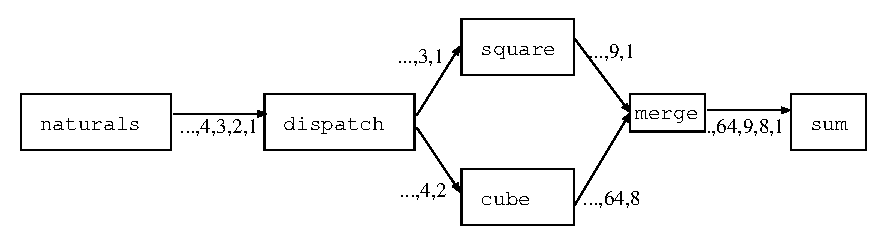
\includegraphics{fig/sqcu.eps}
\caption{木構造プロセス・ネットワーク}
\label{sqcu}
\end{center}
\end{figure}

これは `Nより小さい偶数の平方とNより小さい奇数の立方の総和を求める'
という問題を解くプログラムであった.  
自然数を偶数と奇数に分ける, すなわち入力を分割する(述語dispatch/3によ
って実現される)ディスパッチャプロセス, 
入力の平方を作って出力する(述語square/2によって実現される)フィルタプロセス, 
入力の立方を作って出力する(述語cube/2によって実現される)フィルタプロセス, 
そして(述語merge/3によって実現される)マージャプロセス, といったプロセ
スがこのプログラム中に現れている.  

このプログラムは, 
(naturals/2によって実現される)自然数生成プロセスから(square/2, cube/2
によって実現される)フィルタプロセスまでの, 入力を分割していく木構造, 
それらフィルタプロセスから(sum/2によって実現される)総和計算プロセスま
での, マージャプロセスを使って部分解を集めて全体の解を
作り出す木構造, この二つの木構造プロセス・ネットワークを実現する.  
このような木構造を持ったものがプロセス・ネットワークの基本の一つである.  

前章の復習も兼ねて, 上のプログラム中の各プロセスを実現する述語
についてみていこう.  

まず, ディスパッチャプロセスを実現する述語dispatch/3である.  
%\begin{program}
\begin{Verbatim}[baselinestretch=0.8]
        dispatch([],Odd,Even) :- Odd=[], Even=[].
        dispatch([One|Rest],Odd,Even) :- One mod 2 =:= 0 |
            Odd=[One|OddTail], dispatch(Rest,OddTail,Even).
        dispatch([One|Rest],Odd,Even) :- One mod 2 =\= 0 |
            Even=[One|EvenTail], dispatch(Rest,Odd,EvenTail).
\end{Verbatim}
%\end{program}

第1引数が入力ストリーム, 第2及び第3引数が出力ストリームである.  
入力ストリームから流れてきた入力が
ある条件を満たしたら出力ストリームのどちらかにそれを流す, 
その条件と出力ストリームの組ごとに節が用意されている.  
第1節は, 入力ストリームが閉じられたら出力ストリームを全て閉じて
(再帰的に自らを呼ばないことで)自ら消滅するために用意されている.  
この第1節は後述するようにプログラムの終了判定にとって重要である.  

次にフィルタプロセスを実現する述語square/2,cube/2である.  

%\begin{program}
\begin{Verbatim}[baselinestretch=0.8]
        square([],Out) :- Out=[].
        square([One|Rest],Out) :-
            Square:=One*One, Out=[Square|OutTail], square(Rest,OutTail).
        
        cube([],Out) :- Out=[].
        cube([One|Rest],Out) :-
            Cube:=One*One*One, Out=[Cube|OutTail], cube(Rest,OutTail).
\end{Verbatim}
%\end{program}

第1引数が入力ストリーム, 第2引数が出力ストリームである.  
入力ストリームに流れてきた入力に処理を施し(ここでは平方や立方をとり)
その結果を出力ストリームに流している.  
入力によって施す処理を変えたい時にはディスパッチャと同様に節を幾つか用
意してやれば良い.  
第1節は, ディスパッチャの第1節と同様に, 
入力ストリームが閉じられたら出力ストリームを全て閉じて
自ら消滅するために用意されている.  

フィルタプロセスを幾つか直列につなげばパイプライン・プロセス・ネットワークが
出来る.  入力$N$に対して$N^{6}$を求めるパイプラインは, 次のような述語
で実現できる。

%\begin{program}
\begin{verbatim}
        pipe(In,Out) :- true | square(In,Mid), cube(Mid,Out).
\end{verbatim}
%\end{program}

そして, マージャプロセスを実現する述語merge/3である.  

%\begin{program}
\begin{Verbatim}[baselinestretch=0.8]
        merge([],In2,Out) :- Out=In2.
        merge(In1,[],Out) :- Out=In1.
        merge([Msg|In1],In2,Out) :- Out=[Msg|OutTail], merge(In1,In2,OutTail).
        merge(In1,[Msg|In2],Out) :- Out=[Msg|OutTail], merge(In1,In2,OutTail).
\end{Verbatim}
%\end{program}

入力ストリームである第2引数と第3引数のどちらかに入力が流れてきたら, 
それをそのまま出力ストリームに流す, ということをしているのが第3節, 
及び第4節である.  
第1節, 第2節は, 入力ストリームのどちらかが閉じられ
たら, もう一方を出力ストリームに直結し, 
自ら消滅するために用意されている.  

2本の入力ストリームに同時に入力が流れてきた場合の非決定性(どちらが先
に出力ストリームに流されるかは決められていないこと)はマージャの問題点
ではなく, KL1の特質であることは前章で述べた.  
マージャには入力ストリームの本数の問題があるが, これについては後に
詳しく述べる。

プログラムが大規模になってくると全体を一つのフラットな木構造にする
ことは難しくなる.  そのような場合にはネストした木構造にするのが良い.  

探索問題では, 問題を部分問題に分割し, 各部分問題を各プロセスに解
かせ, その部分問題の解を回収して全体の解を得るという分割統治法がよく
用いられるが, この木構造プロセス・ネットワークはその解法によくマッチす
る.  探索問題の多くはこの木構造を基本としたプロセス・ネットワークで解ける.  

ところで, 上述のsuqare/2, cube/2などの述語によって実現されるプロセスは, 
第1引数の入力ストリームに入力が流れてきた時になって始めて動き出す.  
流れてくる前は中断している.  
つまりこれらのプロセスはプロセス・ネットワークの中でデータ駆動的に
動いている.  しかし, このデータ駆動だけで全てがうまくいくわけではない.  

\subsection{要求駆動とサーバプロセス}
ある与えられた数よりも小さいフィボナッチ数が何個あるかを求めるプログラムを
組んでみよう.  
もし, 与えられた数までのフィッボナッチ数を生成するプロセスが既に
あったとしたら, 
今までのデータ駆動という考え方に基づけば, 
それとカウンタプロセス(入力ストリームを持ち, そこに何個の入力
が流れてきたかをカウントすることを基本動作とするプロセス)をストリームで結ぶ, 
というのが方針の一つとして立つ.  
これに基づいたプログラムが次のものである.  

%\begin{program}
\begin{Verbatim}[baselinestretch=0.8]
        go(Target,Answer) :- true|
            fibonacci(0,1,Stream,Target),
            consume(Stream,0,Answer).
        
        fibonacci(N1,N2,Stream,Target) :- N2 >= Target |
            Stream = [].
        fibonacci(N1,N2,Stream,Target) :- N2 < Target |
            Stream = [N2|StreamN],
            N3 := N1 + N2,
            fibonacci(N2,N3,StreamN,Target).
        
        consume([],Count,Answer) :- true |
            Answer = Count.
        consume([X|StreamN],Count,Answer) :- true |
            CountN := Count + 1,
            consume(StreamN,CountN,Answer).
\end{Verbatim}
%\end{program}
与えられた数までのフィボナッチ数を生成し出力ストリームに流す
ことを基本動作とするプロセスをフィボナッチプロセスとする.   
fibonacci/4がそのフィボナッチプロセスを実現する述語である。第4引数
がその与えられた数, 第3引数が出力ストリームである。

カウンタプロセスを実現するのが述語consume/3である.   
第1引数が入力ストリームであり, カウント結果は第3引数の変数に具体化される.  
ストリームを介してカウンタプロセスがデータ駆動的に動くのが分かる.  
ところで, ここでKL1のゴール実行順序に関する仕様を思い出すと, 
KL1では同一の優先度を持つゴール間の実行順序は特に規定していなかった.  
すると, このプログラムの場合, フィボナッチプロセスが
カウンタプロセスより早く動く可能性がある.  そうすると, 
フィボナッチプロセスが ``\verb!Target!'' までのフィボナッチ数を生成して
終了してから初めてカウンタプロセスが動き出す, つまり, 
 ``\verb!Target!'' が大きい値だった場合は
そのフィボナッチプロセスが大量のメモリを消費してしまう, という可能性がある.  
このフィボナッチプロセスとカウンタプロセスの間で同期を取ってない点で, 
上のプログラムには欠陥がある.  

そこで, このプログラムを要求駆動的\footnote{現在のところ KL1 には要求
駆動を明示する枠組はないので, あくまで記述されたプログラムの意味として
解釈されたい.} に書き換え, プロセス間で同期を取るよ
うにする.  つまり, カウンタプロセスからの要求がある度にフィボナッチ
プロセスが一つだけフィボナッチ数を生成してカウンタプロセスに渡すようにする.  
KL1実行機構を思い出せば, 要求がくるのを待
つようなフィボナッチプロセスはすぐに書けるだろう.  
カウンタプロセスは単なるカウントだけではなく, 
フィボナッチプロセスにフィボナッチ数生成を要求し, ``\verb!Target!'' よ
り小さいかどうかのチェックをする働きをする.  プログラムを次に示す.

%\begin{program}
\begin{Verbatim}[baselinestretch=0.8]
        go(Target,Answer) :- true|
            fibonacci_lazy(0,1,Stream),
            consume(Stream,Target,Answer).
        
        fibonacci_lazy(_,_,[]) :- true | true.
        fibonacci_lazy(N1,N2,[Box|Stream]) :- true |
            N3 := N1 + N2,
            Box = N3,
            fibonacci_lazy(N2,N3,Stream).
        
        consume(Stream,Target,Answer) :-
            NewStream = [Box|Stream],
            consume(Box,Target,0,NewStream,Answer).

        consume(Box,Target,Count,Stream,Answer) :- Target =< Box |
            Stream = [],
            Answer = Count.
        consume(Box,Target,Count,Stream,Answer) :- Target > Box |
            NewCount := Count + 1,
            Stream = [NewBox|NewStream],
            consume(NewBox,Target,NewCount,NewStream,Answer).
\end{Verbatim}
%\end{program}

ストリームの流れが逆であることに注意されたい.  fibonacci\_lazy/3は, 第 
 3 引数のストリームから結果を与える変数 ``\verb!Box!''が到着したら, その
変数にフィボナッチ数を入れ (``\verb!Box!'' にフィボナッチ数を具体化し)
次の結果を与える変数の到着を待つ.  この例題では変数 ``\verb!Box!'' の
到着, 即ち第 3 引数がリストセルにユニファイされることがフィボナッチ数
の計算要求を意味する. 逆に言えばこのストリームが閉じられることがプロセ
スの終了を意味する.  すなわち fibonacci\_lazy/3 は要求駆動的に
フィボナッチ数の計算を行なう述語であり, また答えの容器の到着を待つとい
う意味でデータ駆動でもある.  
一方 consume/5 によって実現されるカウンタプロセスは, 第2節の第 2 ボディ
ゴールで ``\verb!Stream = [NewBox|NewStream]!'' つまりストリーム
に変数 ``\verb!NewBox!'' を流している.  これがフィボナッチプロセスに
`次のフィボナッチ数を生成して ``\verb!NewBox!''に入れろ' と要求を
出していることになるのである.  
そしてその要求の結果がそこに入れられる(具体化されてくる)のを
ガードで待っている.  
尚, プログラムの都合上, consume/3の第 1 ボディゴールで最初の要求を出し
ている.   

未完成メッセージの技法を使って書くことも出来る.  この方式の方が
意味を表現し易く, 特にメッセージ駆動と呼ぶことがある.
  次がメッセージ駆動的に書き直したプログラムである.

%\begin{program}
\begin{Verbatim}[baselinestretch=0.8]
        go(Target,Answer) :- true|
            fibonacci_lazy(0,1,Stream),
            consume(Stream,Target,0,Answer).
        
        fibonacci_lazy(N1,N2,[]) :- true | true.
        fibonacci_lazy(N1,N2,[make(X)|Stream]) :- true|
            X = N2,
            N3 := N1 + N2,
            fibonacci_lazy(N2,N3,Stream).
        
        consume(Stream,Target,Count,Answer) :- true | 
            Stream = [make(X)|StreamN],
            consume(StreamN,Target,Count,Answer,X).
        
        consume(Stream,Target,Count,Answer,X) :- Target =< X |
            Stream = [],
            Answer = Count.
        consume(Stream,Target,Count,Answer,X) :- Target >  X |
            CountN := Count + 1,
            consume(Stream,Target,CountN,Answer).
\end{Verbatim}
%\end{program}

consume/4とconsume/5の二つの述語でカウンタプロセスが実現される.  
カウンタプロセスは `次のフィボナッチ数を生成して ``\verb!X!'' に入れろ'
という要求メッセージである ''\verb!make(X)!'' という未完成メッセージを
ストリーム流す.  そして, 
 ``\verb!X!'' がフィボナッチプロセスによってフィボナッチ数に
具体化されるのを待ち, カウントしたのち, 次の要求を出す.  
 ``\verb!X!'' に具体化される値が ``\verb!Target!'' 以上に
なったら, ストリームを閉じ, 答えを ``\verb!Answer!'' に具体化して, 消
滅する.   

フィボナッチプロセスは, 要求を受けて計算を行ない結果を要求者に返す, という
点でサーバと見ることも出来る.  このサーバもKL1プロセスの重要なプロセス
の一つである.  

\section{解の回収と計算終了判定}
図~\ref{sqcu}のプロセス・ネットワークのように, 
マージャを使って解を収集する木構造を構成することが解回収の基本的方法である.  
この他に差分リストという方法があるが, これは次章で説明される.  

通常の自然なプロセスは入力ストリームが閉じられると出力ストリームを閉じて
自分から消滅する.  マージャも入力ストリームが全て閉じられるとその出力ス
トリームを閉じて消滅する.  
逆に言えば, 出力ストリームが閉じられたということがそのストリームが継っ
ていた部分の計算が終了したことを意味する.  
計算終了の判定はこの出力ストリームが閉じられることを監視することで行う
ことが多い.  しかし, このような自然なプロセスやマージャのみを使って
プロセス・ネットワークを組めない時は, それぞれのネットワークに応じた
計算終了判定法を工夫する必要がある.  その中の一つにショートサーキット
があるがこれは次章で説明される.  

\section{プロセス・ネットワーク構築上の注意点}
この節ではプロセス・ネットワーク構築上の注意点について述べると共に, 
やや高度なプロセス・ネットワークについての説明も行なう.  

\subsection{入出力を分ける}
どの引数が問題記述すなわち入力で, どれがそれに対する解すなわち出力で
あるかをはっきり分け, それを意識しながらプログラミングする.  

%\begin{program}
\begin{Verbatim}[baselinestretch=0.8]
        a([E|X1],Y):-integer(E) |
            E1:=E+1, Y=[E1|Y1], a(X1,Y1).
        a(X,[E|Y1]):-integer(E) |
            E1:=E-1, X=[E1|X1], a(X1,Y1).
\end{Verbatim}
%\end{program}

このようなストリームの向きが決まっていないプロセスも作れることは作れるが, 
このようなプロセスをプロセス・ネットワーク
に入れておくことはバグの元凶であり, またそもそもプロセス・ネットワークの
各ノードの役割や結合形態を云々すること自体, 難しくなる.  
また, KLIC処理系の性能アップの切札として導入予定のKL1プログラム
静的解析は, 入出力のはっきりしないプログラムでは効果的に働かないことも
付け加えておく.  

\subsection{各ノードの役割は単純に}
未完成メッセージの使い方を覚えてしまうと, 章の最初に出てきたプログラム
で, ディスパッチャとマージャ以降の部分を一緒にして次のように書きたくなる.  

%\begin{program}
\begin{Verbatim}[baselinestretch=0.8]
        queer_sum(N,Ans) :-
            naturals(N,Naturals), dispatch_sum(Naturals,Odd,Even,0,Ans),
            square(Even), cube(Odd).
        
        dispatch_sum([],Odd,Even,Sum,Ans) :- Odd=[], Even=[], Ans=Sum.
        dispatch_sum([One|Rest],Odd,Even,Sum,Ans) :- One mod 2 =\= 0 |
            Odd=[make(One,Ret)|OddTail],
            dispatch_sum(Rest,OddTail,Even,Sum,Ans,Ret).
        dispatch_sum([One|Rest],Odd,Even,Sum,Ans) :- One mod 2 =:= 0 |
            Even=[make(One,Ret)|EvenTail],
            dispatch_sum(Rest,Odd,EvenTail,Sum,Ans,Ret).

        dispatch_sum(Rest,Odd,Even,Sum,Ans,Ret) :- wait(Ret) |
            SumN := Sum+Ret,
            dispatch_sum(Rest,Odd,Even,SumN,Ans).

        square([]) :- true | true.
        square([make(One,Square)|Rest]) :- true |
            Square:=One*One, square(Rest).

        cube([]) :- true | true.
        cube([make(One,Cube)|Rest]) :- true |
            Cube:=One*One*One, cube(Rest).
\end{Verbatim}
%\end{program}

このプログラムによって実現されるプロセス・ネットワークは図~\ref{sqcu2}
のようになる.  

\begin{figure}
\begin{center}
% \epsfile{file=sqcu2.eps}
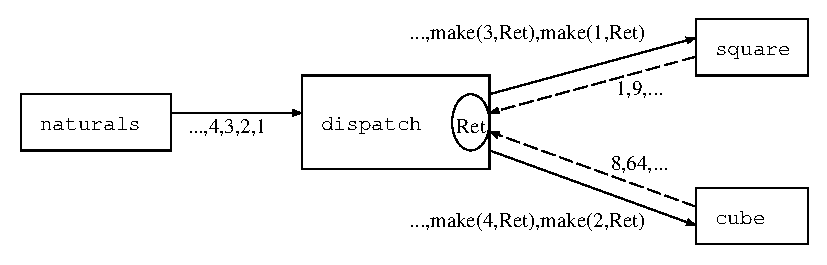
\includegraphics{fig/sqcu2.eps}
\caption{木構造プロセス・ネットワーク2}
\label{sqcu2}
\end{center}
\end{figure}

dispatch\_sum/5及びdispatch\_sum\_6は, 二つの述語で一つのプロセスを実現し, 
入力の分割と, 
square/1で実現されるプロセス及びcube/1で実現されるプロセスへの
要求メッセージ送出, そして平方と立方の合計の保持も行なっている.  
この場合はプログラム全体の規模が小さいので問題ないが, 一般に規模の大きなプ
ログラムでこのような一人何役も兼ねたプロセスを多用すると, プログラム
全体の構造が見えにくくなる.  後に述べるようなサーバプロセスを作る必要性
のある場合はいざ知らず, プログラム全体を素直な木構造で表現出来る場合は, 
できる限りマージャ, フィルタ, ディスパッチャといった単純な構成要素から
考えた方が良い.  

ネットワーク構造が大きくなってくると, 当然モジュール化が必要になる.  
木構造のサブネットワークをモジュールとしてまとめ, メインネットワークのひとつの
ノードと考えるのが便利である.  このときも各サブネットワー
クがマージャ, フィルタ, ディスパッチャなどの役割を果たすようにすると, 
プログラム全体がネストした木構造になり, 構造がわかりやすくなる.

\subsection{部分木は直接通信させない}
部分問題を解く計算を通して得られたデータを, 別の部分問題を解くところで
も活用したくなる場合は少なくない.  このような場合も, サブネットワーク
すなわち部分木どうしが直接通信するようにプログラムすると, 
プログラムの全体の木構造が崩れて, 構造が把握しにくくなる.  

プログラム全体は木構造のままで, 部分木間でデータを共有したい場合は, 共
有データのためのサーバプロセスを置き, ここを経由して通信するようにする
と, 構造を把握しやすくなる.  
すなわち, 図~\ref{server}の左のようなプロセス・ネットワークでなく, 右の
ようなプロセス・ネットワークを構成するのである。
プログラムは以下のようになるだろう.  

%\begin{program}
\begin{Verbatim}[baselinestretch=0.8]
        p(I, O) :-
            decompose(I, I1, ..., In),
            merge({S1, ..., Sn}, S),
            shared_data_server(S),
            p1(I1, S1, O1),
            ...,
            pn(In, Sn, On),
            compose(O1, ..., On, O).
\end{Verbatim}
%\end{program}

\begin{figure}
\begin{center}
% \epsfile{file=server.eps}
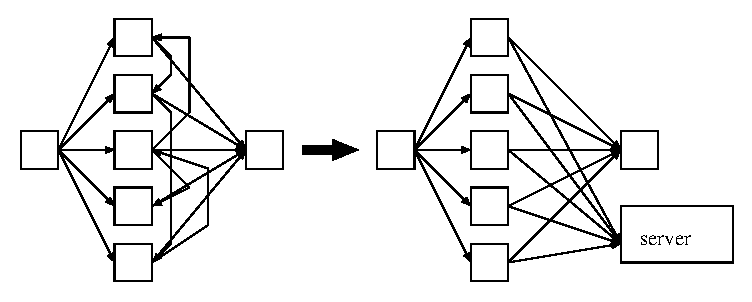
\includegraphics{fig/server.eps}
\caption{サーバプロセスを通した通信へ}
\label{server}
\end{center}
\end{figure}

決してとるべきでない通信形態は `部分木のうち最初に解を見つけたものが他
の部分木の計算をやめさせる' というような方法である.  このような形態を
とると複数の部分木がほぼ同時に解を見つけた場合に, いつでも正しく動作さ
せるようにするのが難しくなる.  解が見つかった, という事実は共有データ
である.  解を見つけた部分木は共有データのサーバに連絡し, このサーバが
他の部分木を終了させるようにするのが良い.  一般に, 競争条件は原則とし
てストリームのマージ機構に一元化すべきである.  

\subsection{ループは避ける}
ストリーム通信を使えばループ構造の正しいプログラムも書けるが, ループ構
造はデッドロックの温床になるので乱用すべきではない.  ループがなければ
デッドロックはあり得ない.  

直接的なループ構造を避けるためには, やはりサーバ方式が有効である.  パ
イプライン構造の下流から結果を直接上流にフィードバックするのではなく,  
データベースであるサーバプロセスに送ることとし, 上流からはこれにアクセ
スして情報を得るようにすると, 基本的なプロセス構造がすっきりして把握し
やすくなることが少なくない.  

\subsection{カオスなネットワークはやめよう}
今まで述べたプロセス・ネットワークの構築に関する事柄を一つにまとめると, 
主構造は(パイプラインを含んだ)ネストした木構造で, サーバを通して
副次ラインが張ってある図~\ref{network}のようなプロセス・ネットワーク, 
ということになる.  

\begin{figure}
\begin{center}
% \epsfile{file=network.eps}
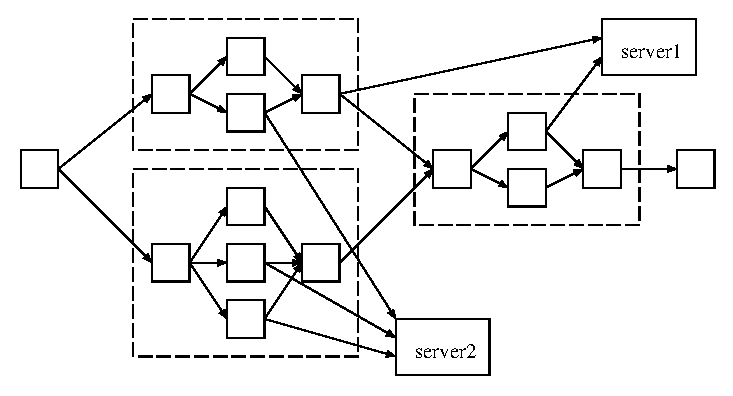
\includegraphics{fig/network.eps}
\caption{プロセス・ネットワーク}
\label{network}
\end{center}
\end{figure}

もちろん, この形に固執することはない.  アルゴリズムに応じて, 
なるべく明確かつ単純な構造のKL1プログラムを作ることを心がけるべきである.  
プログラムを書き始める前に, プロセス・ネットワークのデザインをさぼって 
成りゆきで書き始めてしまうと, カオスなネットワークが出来ることに
なってしまう.  

\subsection{マージャ}
プロセス・ネットワークの重要な要素であるマージャには, 
入力ストリームの本数という問題点がある.  
次のマージャプログラムは入力ストリーム2本用のものである.  

%\begin{program}
\begin{Verbatim}[baselinestretch=0.8]
        merge([],In2,Out) :- Out=In2.
        merge(In1,[],Out) :- Out=In1.
        merge([Msg|In1],In2,Out) :- Out=[Msg|OutTail], merge(In1,In2,OutTail).
        merge(In1,[Msg|In2],Out) :- Out=[Msg|OutTail], merge(In1,In2,OutTail).
\end{Verbatim}
%\end{program}

入力ストリームを3本, 4本と増やしたい場合には, 
3本用マージャ, 4本用マージャと一つ一つプログラムを用意してやるか, 
2本用マージャでもって木構造をつくる
(図~\ref{merge}参照)かしなければならない.  
前者の方法では, プログラムサイズが大きくなるという問題点がある.  
後者の方法では, 入力ストリームが$N$本あった場合, 
最低でも深さ$\log N$の木構造を構成してやる必要があり, 
実行時の効率も悪くなる\footnote{一つのメッセージがマージャ木構造を通り
抜けるのには, 最悪, その木の深さに比例する時間と計算量がかかる}.  

\begin{figure}
\begin{center}
% \epsfile{file=merge.eps}
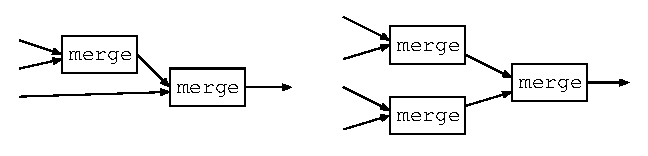
\includegraphics{fig/merge.eps}
\caption{マージャのツリー構造}
\label{merge}
\end{center}
\end{figure}

この問題を解決するためにKLIC処理系では組み込み述語として
マージャをサポートする.  

これは, ``\verb!merge(In,Out)!'' という形で呼び出し, ``\verb!In!'' に入力スト
リームを要素とするベクトルをunifyしてやることで利用出来る.  例えば, 
以下の二つのボディゴールによって,  ``\verb!In1,In2,In3!'' を入力ストリーム, 
 ``\verb!Out!'' を出力ストリームとする入力ストリーム3本用マージャが用
意出来る.   

%\begin{program}
\begin{Verbatim}[baselinestretch=0.8]
            merge(In,Out),
            In = { In1, In2, In3 },
\end{Verbatim}
%\end{program}


\section{やや高度なネットワークの組み方}

%KL1には古くから暗黙引数マクロという技法がある.  詳しくはPIMOSマニュア
%ル参照のこと\footnote{現時点で暗黙引数マクロに関する最も詳しい解説が
%記載されている}.  暗黙引数マクロを使えば, 
%\begin{itemize}
%\item
%親ゴールからすべての子ゴールに渡すだけの引数や, パイプライン構造プログ
%ラムでフィルタをつなぐだけのための引数は, それぞれ shared 型, oldnew 
%型の暗黙引数として宣言しておけば, いちいち記述せずに済みつづりを誤る可
%能性もない.  
%\item
%ストリーム引数については, stream 型暗黙引数と宣言しておけばプロセス終
%了時 (ボディゴールのない節を選んだ時) に自動的に閉じられるので, 閉じ忘
%れの可能性はない.  
%\end{itemize}
%となることから, プロセス・ネットワークを組む際に入れる典型的なバグである
%変数綴の間違いやストリームの閉じ忘れなどを最初から入れずに済む.  
%
%また, 状態変数の追加時には,, 実際にその状態変数を参照する部分と暗黙引数宣言部
%だけを訂正すれば良く, 単に受け渡しているだけの中間部分には手を入れなく
%て良いので, 改訂時にバグを混入させる危険性も減る.  

デバッグのための状態問い合わせストリームというものがある.  
これは全てのプロセスを串刺しにしたストリーム(図~\ref{jotai})で, 
これをプロセス・ネットワークに組み込んでおき, 
デバッグ時にこのストリームを通して各プロセスの状態をかき集めてデバッグ
に役立てるものである.  

\begin{figure}
\begin{center}
% \epsfile{file=jotai.eps}
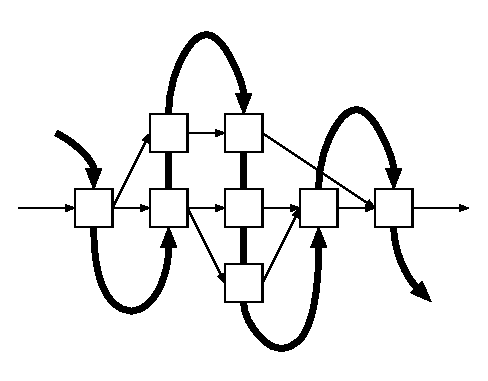
\includegraphics{fig/jotai.eps}
\caption{状態問い合わせ用ストリーム}
\label{jotai}
\end{center}
\end{figure}

次に, プロセス・ネットワークの使い方の面白い例を一つ挙げよう.  

\begin{figure}
\begin{center}
% \epsfile{file=path.eps}
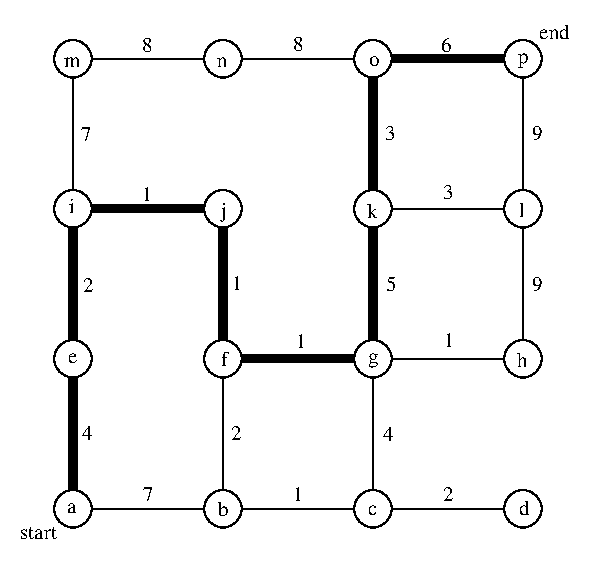
\includegraphics{fig/path.eps}
\caption{コスト付き経路網}
\label{path}
\end{center}
\end{figure}

最適経路問題とは, 図~\ref{path}のようなノード間をつないだコストつき
経路網が存在する時に, 開始点から終了点までの経路のうち, 
コスト最小のものを求めるという, 探索問題の一つである.  
探索問題であるから, これを部分問題に分割して, 
各部分問題にプロセスを割り当てて, というように今まで述べてきた考え方
に沿って問題を解いていくこともできるのだが, もっと直接的かつ大胆に, 
経路上の各ノードをプロセス, ノード間のアークを双方向ストリーム
\footnote{実際には向きが逆の2本の単方向ストリームとして実現する}, として
解くことも出来る.  
各ノードプロセスは自分から伸びているアークのコストを知っている.  
また, 各ノードはそれまでに判明した, 開始点から自分までの最適(コスト最小)経路
とそのコストの対を保持している.  
そして, それよりも低コストな, 新たな自分までの最適経路を見つけた場合は
その新た最適経路とコストの対でもって保持している対を更新し, 
自分に直接継っているノードにその新たな対をメッセージとして送る.  
例えば, ノードfがある時点で, 自分までの最適経路がコスト$7+2=9$の
経路a$\rightarrow$b$\rightarrow$fだと思っている(その対を保持している)とする.  
そこへ, ノードjから "ノードjまでの最適経路は
今のところa$\rightarrow$e$\rightarrow$i$\rightarrow$jで, そのコストは
$7$だと分かった”という意味のメッセージ 
\{a$\rightarrow$e$\rightarrow$i$\rightarrow$j,7\} を受けとったら, 
自分までの最適経路が今まで思っていたb回りの経路でなく, j回りの経路であ
ることが分かる.  そこで, 保持している対をそのj回りのものに更新し, 
ノードb, g, jに
メッセージ\{a$\rightarrow$e$\rightarrow$i$\rightarrow$j$\rightarrow$f,8\}
を送る.  開始点aがノードb,eにメッセージを送ることに始まって, このようなメ
ッセージがプロセス・ネットワーク上を流れ回った後には, 各ノードプロセスに
は開始点からそのノードまでの最適経路とそのコストの対が保持されている.  
計算の終了は全てのメッセージがプロセス・ネットワークから消滅したことで
判定する(この判定は次章で述べるショートサーキットという技法が使われる
がここでは述べない).  

\section{演習問題}
演習問題の前に画面への出力方法を示す.  
プログラムの実行結果を出力するためのストリームを確保する組み込み述語は
io:outstream/1 である.  
そのストリームに ``\verb!print(X)!'' というメッセージを流せば, 
変数 ``\verb!X!'' に具体化されている値が画面に出力される。
改行するには, ``\verb!nl!'' というメッセージを送る.
例えば, 以下のゴールで, 変数 ``\verb!X!'' に具体化されている値を出力し, 
改行する. 

%\begin{program}
\begin{verbatim}
            io:outstream([print(X),nl]),
\end{verbatim}
%\end{program}

\exercise{フィボナッチ数の平方と立方の総和}
与えられた整数\verb!Target!より小さな全てのフィボナッチ数について, 
平方と立方の総和を求めるプログラムを作成し, \verb!Target!=100
とした時の実行結果を出力せよ。

\exercise{$2^{l} \times 3^{m} \times 5^{n}$}
与えられた整数\verb!Target!より小さい正の整数で, 
$2^{l} \times 3^{m} \times 5^{n}$($l,m,n$は負でない整数)という形で表す
ことの出来るものが幾つあるか求めるプログラムを作成し, 
\verb!Target!=10000とした時の実行結果を出力せよ。
但し, パイプライン型のプロセス・ネットワークを使ってデータ駆動で書くこと.  
\verb!X!の\verb!Y!に対する剰余が\verb!Z!に等しいことの判定
には``\verb! X mod Y =:= Z !'', 
等しくないことの判定には ``\verb! X mod Y =\= Z !'' とガードに書けば良い.  
\verb!X!の\verb!Y!に対する商を\verb!Z!に具体化するには, 
 ``\verb! Z := X / Y !''というボディゴールを書けば良い.  

%\setcounter{exercise}{0}

\answer{フィボナッチ数の平方と立方の総和}
データ駆動で書いたものが次のプログラムである.  
本文中に出てきた fibonacci/4, square/2, cube/2 merge/3 sum/2を
ストリームでつなげば良い.  

%\begin{program}
\begin{Verbatim}[baselinestretch=0.8]
        :- module main.

        main :- true|
            main(100,Answer),
            io:outstream([print(Answer),nl]).

        main(Target,Answer) :- true|
            fibonacci(0,1,Fibo,Target),
            square(Fibo,Squares), cube(Fibo,Cubes),
            merge(Squares,Cubes,Both),
            sum(Both,Answer).
\end{Verbatim}
%\end{program}

\verb!Target!=100とした時の答えは, 935596である.  

要求駆動, あるいはメッセージ駆動で書くのなら, 
フィボナッチプロセスに要求を出し, その結果であるフィボナッチ数を
square/2, cube/2 で実現されるフィルタプロセスに配るプロセスを
組み込むのが良い.  
以下のプログラムはメッセージ駆動で書いたものである.  
square/2, cube/2, merge/3, sum/2は本文中と同じである.  

%\begin{program}
\begin{Verbatim}[baselinestretch=0.8]
        :- module main.

        main :- true|
            main(100,Answer),
            io:outstream([print(Answer),nl]).

        main(Target,Answer) :- true|
            fibonacci_lazy(0,1,Stream),
            dispatch(Stream,Target,Fibo),
            square(Fibo,Squares), cube(Fibo,Cubes),
            merge(Squares,Cubes,Both),
            sum(Both,Answer).

        fibonacci_lazy(N1,N2,[]) :- true | true.
        fibonacci_lazy(N1,N2,[make(X)|Stream]) :- true|
            X = N2,
            N3 := N1 + N2,
            fibonacci_lazy(N2,N3,Stream).

        dispatch(Stream,Target,Fibo) :- true | 
            Stream = [make(X)|StreamN],
            dispatch(StreamN,Target,Fibo,X).

        dispatch(Stream,Target,Fibo,X) :- X >= Target|
            Stream = [],
            Fibo = [].
        dispatch(Stream,Target,Fibo,X) :- X < Target|
            Fibo = [X|FiboN],
            dispatch(Stream,Target,FiboN).
\end{Verbatim}

\answer{$2^{l} \times 3^{m} \times 5^{n}$}
入力を正の整数\verb!N!で割れるだけ割った数を出力するフィルタを用意する.  
例えば, \verb!N!=2 としたものに12を通すと3を出力するようなフィルタである.  
また, 入力のうち1が何個あったかをカウントするカウンタプロセスを用意する. 
そして, 
\verb!N!=2としたフィルタ, \verb!N!=3としたフィルタ, \verb!N!=5としたフィルタ, 
これらをつないだパイプラインの前に自然数生成プロセス, 
後ろにカウンタプロセスをつないで, 図~\ref{pipeline}のような
プロセス・ネットワークを作れば, 問題の式で表せる数が幾つあるかを
計算するプロセス・ネットワークが出来る.  

\begin{figure}
\begin{center}
% \epsfile{file=pipeline.eps}
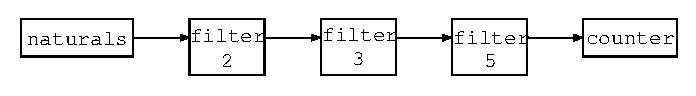
\includegraphics{fig/pipeline.eps}
\caption{}
\label{pipeline}
\end{center}
\end{figure}

%\begin{program}
\begin{Verbatim}[baselinestretch=0.8]
        :- module main.

        main :- true|
            main(10000,Answer),
            io:outstream([print(Answer),nl]).

        main(Target,Answer) :- true|
            naturals(1,Target,Stream0),
            filter(2,Stream0,Stream1),
            filter(3,Stream1,Stream2),
            filter(5,Stream2,Stream3),
            counter(0,Stream3,Answer).

        naturals(N,M,List) :- N>=M |
            List=[].
        naturals(N,M,List) :- N<M  |
            List=[N|Rest],
            N1:=N+1,
            naturals(N1,M,Rest).

        filter(_,[],Out) :- true |
            Out = [].
        filter(X,[E|InN],Out) :- true |
            filter(X,E,InN,Out).

        filter(X,E,InN,Out) :- E mod X =:= 0 |
            EN := E / X,
            filter(X,EN,InN,Out).
        filter(X,E,InN,Out) :- E mod X =\= 0 |
            Out = [E|OutN],
            filter(X,InN,OutN).

        counter(C,[],Res) :- true |
            Res = C.
        counter(C,[1|InN],Res) :- true |
            CN := C + 1,
            counter(CN,InN,Res).
        counter(C,[E|InN],Res) :- E =\= 1 |
            counter(C,InN,Res).
\end{Verbatim}
%\end{program}

\verb!Target!=10000とした時の答えは,174である.  

\chapter{差分リストの使い方}
\section{クイックソートの原理}
クイックソートは, ソートすべき数値の集合の中から一つを取りだし, 
その数よりも小さい集
合と大きい集合との2つに分け,それぞれの集合の中で, さらに一つを取りだし, その
中で大きい集合と小さい集合とに再帰的に分類していく方法である. クイックソート
を使えば,  NlogN 回の比較回数で済ますことが期待できる.  \par

\begin{figure}[htbp]
  \begin{center}
% \epsfile{file=dlt1.eps,width=.5\textwidth}
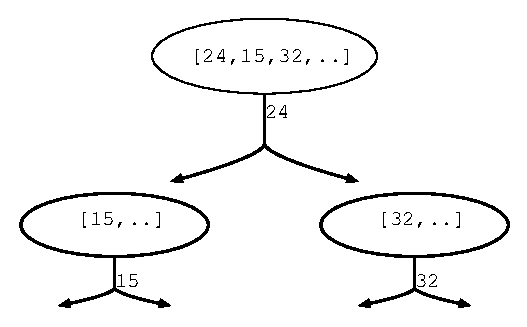
\includegraphics[width=.5\textwidth]{fig/dlt1.eps}
    \caption{クイックソート}
  \end{center}
\end{figure}

  まず,  リストで与えられた数列の中から数値を1つ取り出して,  2つの集合に分
けることを考える.(とりあえず,数値が同じだった場合のことは考えない)

\begin{Verbatim}[baselinestretch=0.8]
  qsort([H|T]) :- true | compare(H,T).

  compare(V,[H|T]) :- V > H | compare(V,T), 小さい方の集合に H を加える.
  compare(V,[H|T]) :- V < H | compare(V,T), 大きい方の集合に H を加える.
\end{Verbatim}

とすればよい.  しかし,  グローバル変数という概念は, KL1の世界にはないため, 
集合を蓄える場所として KL1 ではゴールの引数を使用(利用)する. 

\begin{Verbatim}[baselinestretch=0.8]
   qsort([H|T]) :- true | compare(H,T,L_small,R_small).

   compare(V,[H|T],L_small,R_large) :- V > H |
           compare(V,T, L_small に H を加えたもの, R_large).
   compare(V,[H|T],L_small,R_large) :- V < H |
           compare(V,T, L_small, R_large に H を加えたもの).
\end{Verbatim}

  では, L\_{}small に H を加えたものをどう表現すればよいだろう.  長さがわから
ない
場合はリストで表現するとよい. (長さがわかっているような場合には,複合項や
ベクタを利用する方法もある. )例えば,  
 1 と 2 と 3 の集合は [1,2,3] と長さ3のリストで表現すればよい.  \par
リストで情報をどのような順番で記録して行けばよいのであろうか.  この記録の仕方
には,  2つの方法がある.  スタックとキューである.  

\begin{itemize}
 \item LIFO法(スタック)\\
  データを次々に積み上げて行く方法である.  
\begin{figure}[htbp]
  \begin{center}
%     \epsfile{file=dlt2.eps,width=.5\textwidth}
    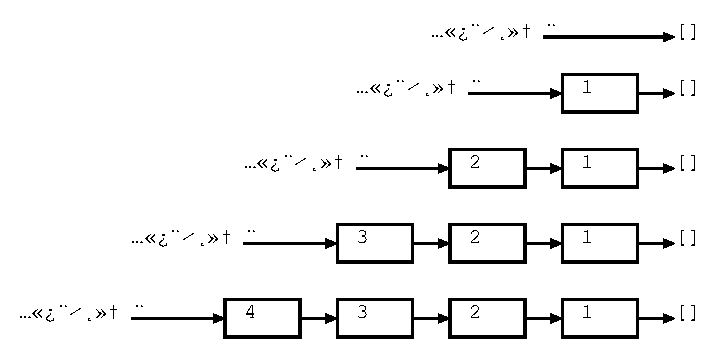
\includegraphics[width=.5\textwidth]{fig/dlt2.eps}
    \caption{LIFO}
  \end{center}
\end{figure}

   述語 compare の場合には,  L\_{}small に H を加えたものは
    [H$\mid$L\_{}small] になる.
   集合の初期値は,  空集合であるので,  [](空リスト)にしなければならない.  

\begin{Verbatim}[baselinestretch=0.8]
   qsort([H|T]) :- true | compare(H,T,[],[]).

   compare(V,[H|T],L_small,R_large) :- V > H | New_L = [H|L_small],
       compare(V,T,New_L,R_large).
   compare(V,[H|T],L_small,R_large) :- V < H | New_R = [H|R_large],
       compare(V,T,L_small,New_R).
\end{Verbatim}

 \item FIFO法(キュー)\\
   データを次々に後尾に挿入して行く方法である. 

\begin{figure}[htbp]
  \begin{center}
%     \epsfile{file=dlt3.eps,width=.45\textwidth}
    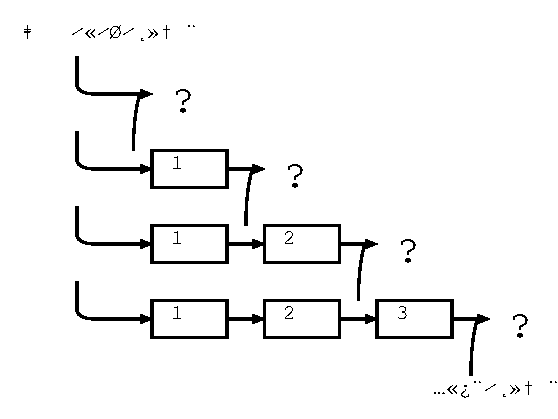
\includegraphics[width=.45\textwidth]{fig/dlt3.eps}
    \caption{FIFO}
  \end{center}
\end{figure}

   L\_{}small に H を加えたものは,L\_{}small を [H$\mid$次に加える変数] にする.
   また最後は,  [](空リスト)で集合を閉じるようにしなければならない.  \par

\begin{Verbatim}[baselinestretch=0.8]
   qsort([H|T]) :- true | compare(H,T,ExL_small,ExR_large).

   compare(V,[]   ,L_small,R_large) :-  true | L_small = [], R_large = [].
   compare(V,[H|T],L_small,R_large) :- V > H | L_small = [H|New_L],
       compare(V,T,New_L,R_large).
   compare(V,[H|T],L_small,R_large) :- V < H | R_large = [H|New_R],
       compare(V,T,L_small,New_R).
\end{Verbatim}

\end{itemize}
  これらの記憶方法には,  共に異なる特徴がある. 
LIFO法では,  実行中のゴールが,  生成したデータ
の集合を常に参照でき,  集合内のデータを検査しながら仕事ができる.  またデ
ータの入ってきた順とは,  逆にデータが並ぶので,データの並びを逆転するのに
も向いている. 
  一方,  FIFO法では,実行中のゴールは,  生成したデータの集合を参照できな
いが,外部のゴールから,  生成したデータが見え,  並列処理できる(並列性があ
る).  \par
  どちらの方法がよいかは,  プログラマがアプリケーションを見て判断する.  
  この場合,LIFO法での利点はないので,  並列性のある
  FIFO法の方が好ましいようである. (LIFO法でもできないわけではない.)

  これで, 数を 1つ取り出して,  それよりも小さいものの集合と大きいものの集合が
得られた.
次に小さいもの集合の中で,  さらに数を 1つを取り出して,  同様に分類するようにしなけ
ればならない.  再分類する処理方法は全く同じなので,  もう一度最初から呼ぶように
すればよい.  

\begin{Verbatim}[baselinestretch=0.8]
   qsort([H|T]) :- true | compare(H,T,L_small,R_large),
        qsort(L_small), q_sort(R_large).

   compare(V,[]   ,L_small,R_large) :-  true | L_small = [], R_large = [].
   compare(V,[H|T],L_small,R_large) :- V > H | L_small = [H|New_L],
       compare(V,T,New_L,R_large).
   compare(V,[H|T],L_small,R_large) :- V < H | R_large = [H|New_R],
       compare(V,T,L_small,New_R).
\end{Verbatim}

  このプログラムは,  動作中は図のように ``compare"が木のノードとして,足(ゴー
ル同士がつながるストリーム)を2本持ち,  末端に ``qsort"つながるような形に
なる.  

\begin{figure}[htbp]
  \begin{center}
%     \epsfile{file=dlt4.eps,width=.6\textwidth}
    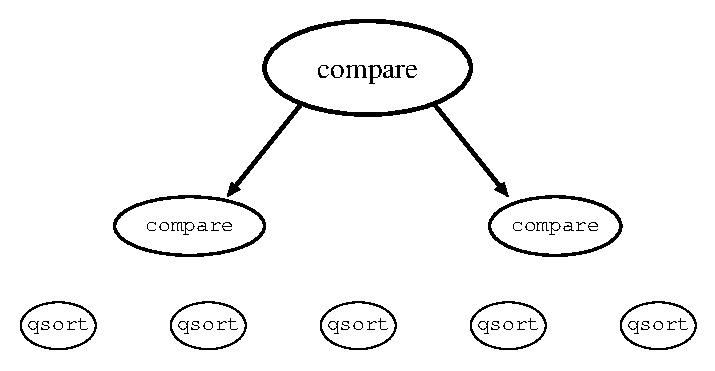
\includegraphics[width=.6\textwidth]{fig/dlt4.eps}
    \caption{Binary Tree}
  \end{center}
\end{figure}

  このプログラムを述語名を木の名前にして,  値が同一だった場合の処理やデータ
の終わりの処理を付け加えれば次のように完成する.  

\begin{Verbatim}[baselinestretch=0.8]
  node([],V,L,R) :- true | L = [], R = [].
  node([H|T],V,L,R) :-  H > V  | R = [H|NR], node(T,V,L,NR).
  node([H|T],V,L,R) :-  H < V  | L = [H|NL], node(T,V,NL,R).
  node([H|T],V,L,R) :- H =:= V | node(T,V,L,R).

  terminal([])    :- true | true.
  terminal([H|T]) :- true | node(T,H,L,R), terminal(L), terminal(R).
\end{Verbatim}


\section{差分リスト}
  先程の例では,  ソートされた木を生成することはできたが,  ソートされた結果を
外に出していない.  結果を外に出す時には,先程のFIFO法があるが,  それだけでは
結果を出力する窓口が一つしかない.  すでにプログラムは,  並列性を持ったプログ
ラムであり,  並列に結果を並べられるような工夫が必要となる.  

\begin{figure}[htbp]
  \begin{center}
%     \epsfile{file=dlt5.eps,width=.8\textwidth}
    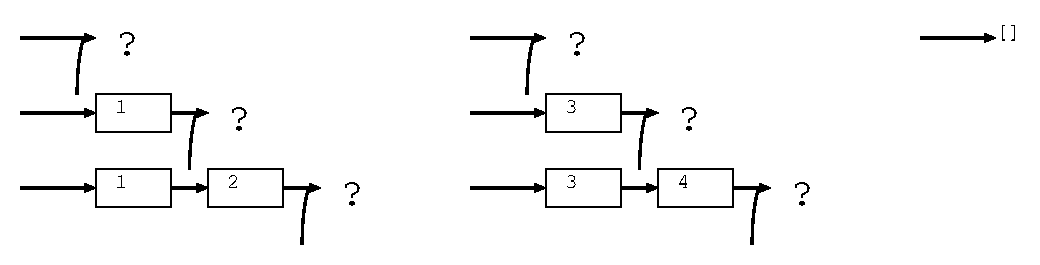
\includegraphics[width=.8\textwidth]{fig/dlt5.eps}
    \caption{並列に解が出力}
  \end{center}
\end{figure}

ここで, 出力のための引数とは別に,  他のゴールの出力をつなぐための新たな変数を
1 つ設ける.  これにより,  複数の結果出力を並行させ,  それらをつなぐようにで
きる.  このように出力のための変数を2つ(直接出力のための変数と,以降のゴール
の出力をつなぐための変数)を持ち回って,  並列処理を損なうことなく結果を収集
する技法を{\dg 差分リスト}という.  

\begin{figure}[htbp]
  \begin{center}
%     \epsfile{file=dlt6.eps,width=.8\textwidth}
    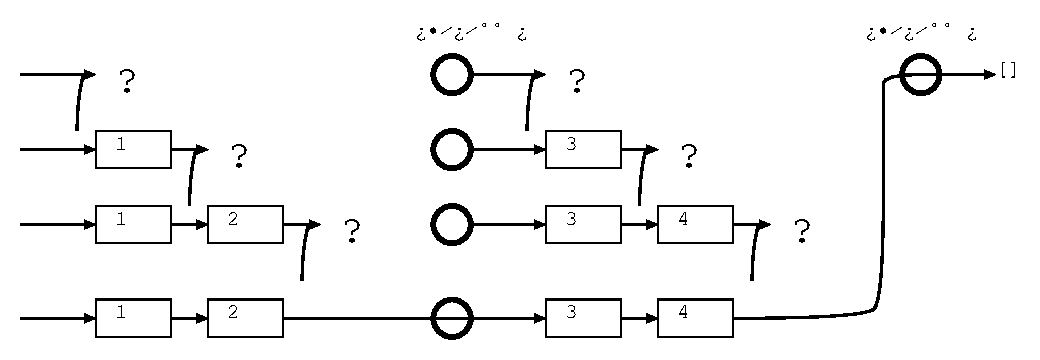
\includegraphics[width=.8\textwidth]{fig/dlt6.eps}
    \caption{解の連結}
  \end{center}
\end{figure}

  差分リストは,  ノード間の解を集めるのに有効な技法である.  クイックソートの解
を出力するため,  差分リストの2引数(解を出力するための引数と解同士をつなぐ新た
な変数の引数)を加える.  プログラムは次のようになる.  

\begin{Verbatim}[baselinestretch=0.8]
  qsort(In,Out) :- true | terminal(In,Out,[]).

  node([]   ,V,L,R,Xs,Ys) :-  true   | L = [], R = [], Xs = [V|Ys].
  node([H|T],V,L,R,Xs,Ys) :-  H > V  | R = [H|NR], node(T,V,L,NR,Xs,Ys).
  node([H|T],V,L,R,Xs,Ys) :-  H < V  | L = [H|NL], node(T,V,NL,R,Xs,Ys).
  node([H|T],V,L,R,Xs,Ys) :- H =:= V | node(T,V,L,R,Xs,Ys).

  terminal([]   ,Xs ,Ys) :- true | Xs = Ys.
  terminal([H|T],Xs0,Ys) :- true |
       terminal(L,Xs0,Xs1), node(T,H,L,R,Xs1,Xs2), terminal(R,Xs2,Ys).
\end{Verbatim}

  ``qsort'' から ``terminal''に渡された差分リストは最終的に ``node''に渡り,
入力ストリームが閉じられた時に解を出力するようにしている.
  ここで ``node'' は,  差分リストを持ち回っているが,その差分リストを処理し
ているのは, 入力ストリームが閉じられた時にのみ差分リストの単一化が
実行されている.  
  単一化を処理するのはいつでもよいから,  ``node'' を呼び出している ``terminal''
 の中で処理することができ,  
``node'' への引数として渡す必要がないことがわかかる.  

  このようにクイックソートの原理を素直に書き下し,  整形していくと,  
次のような(例題プロ
グラムとしてよく出される)クイックソートのプログラムになる. 
(例題では node $\rightarrow$ split or partition , terminal $\rightarrow$ qsort 
になっていることが多い.)

\begin{Verbatim}[baselinestretch=0.8]
  qsort(In,Out) :- true | terminal(In,Out,[]).

  node([]   ,V,L,R) :-  true   | L = [], R = [].
  node([H|T],V,L,R) :- H > V   | R = [H|NR], node(T,V,L,NR).
  node([H|T],V,L,R) :- H < V   | L = [H|NL], node(T,V,NL,R).
  node([H|T],V,L,R) :- H =:= V | node(T,V,L,R).

  terminal([]   ,Xs ,Ys) :- true | Xs = Ys.
  terminal([H|T],Xs0,Ys) :- true |
       terminal(L,Xs0,Xs1), node(T,H,L,R), Xs1 = [H|Xs2], terminal(R,Xs2,Ys).
\end{Verbatim}

\section{ショートサーキット}
  差分リストは,  結果を出力するための有力な方法だが,  出力された結果が全て求ま
ったことは,  結果が求まったタイミングを得ることができる方法であると言える.  
  すなわち,  差分リストの考え方は(結果を見たいのではなく, )処理終了のタイミ
ングを得たい時にも応用が効く.  
  各ゴールは,  ある(通常, 処理が終了した)タイミングで差分リストの2引数を閉じる
ように(単一化)すれば,  外から差分リストの先頭を参照しているゴールが,  
差分リストの終端
が見えることで,  すべてのゴールの処理が終了したタイミング得ることができる.  

\begin{figure}[htbp]
  \begin{center}
%     \epsfile{file=dlt9.eps,width=.8\textwidth}
    \includegraphics[width=.8\textwidth]{fig/dlt9.eps}
    \caption{ショートサーキット}
  \end{center}
\end{figure}
  プログラムでは,  下記のようにして監視ゴールが,  仕事の終了のタイミングを
つかむ.

\begin{Verbatim}[baselinestretch=0.8]
  job :- inspector(C0),
        worker1( ...    ,C0,C1),
        worker2( ...    ,C1,C2),
        .
        .
        workerN( ...    ,CN,[]).

  inspector(W) :- wait(X) | next_job.
\end{Verbatim}

  こうして,  差分リストのようにゴール間に2引数を付加してタイミングを得るための
技法を{\dg ショートサーキット}と呼ぶ.  

\section{出力ストリーム}

KL1 は並列言語であり,  一般の手続型言語のように処理順が明確に規定されて
いるわけではない.
  (KL1 ではゴールの実行順を規定するのは, ゴール間の引数の同期の
機構だけである. )\par
  このような並列言語でデータを出力するような場合に,  
単純にデータを出力するような機能を用意してプログラムを書いてしまうと, 
一つしかない出力装置を取り合うことになってしまう.

\begin{figure}[htbp]
  \begin{center}
%     \epsfile{file=dlta.eps,width=.6\textwidth}
    \includegraphics[width=.6\textwidth]{fig/dlta.eps}
    \caption{アクセスの競合}
  \end{center}
\end{figure}

一つしかない共有資源を,  複数の処理単位(ゴール)が並列にアクセ
スするような場合には,  
あらかじめ一本のストリームを用意して各ゴールからのアクセスを差分リスト
で渡すようにするか,  アクセスを取りまとめるような仲介者({\em merger})
を介在させて,  最終的に一本のストリームにまとめるかしなければならない.

\begin{figure}[htbp]
  \begin{center}
%     \epsfile{file=dltb.eps,width=.6\textwidth}
    \includegraphics[width=.6\textwidth]{fig/dltb.eps}
    \caption{共有資源へのアクセス}
  \end{center}
\end{figure}

  このような事情から klic では, 直接出力装置にアクセスする手段はなく, 
一本のアクセス要求ストリームを処理するデータ出力のための組
込み述語({\em outstream/1})を提供している.

\begin{Verbatim}[baselinestretch=0.8]
   job :- true | work(O), io:outstream(O).

   work(O) :- true | 
      worker1(  ...  ,O,O1),
      worker2(  ...  ,O1,O2),
      .
      .
      workerN(  ...  ,On,[]).
\end{Verbatim}

 outstream が受け入れるコマンドは print/1(引数の内容出力要求)
 と nl(改行要求)がある. 
なお, print/1 で引数の内容が具体化していない場
合には同期の機構が働いて待ち合わせするようになっており,  具体化されるまで
実際の出力はされない.




\exercise{データ記録方法の練習}
バイナリソートのプログラムをLIFO法で解を出力するプログラムを書いて, 
FIFO法の場合と比較せよ. \\

\exercise{ソートの練習}
\label{sort1}
下記のような重複のある数列を入力として,  重複なしの昇順のソートをして,  数と
出現回数を出力せよ.  
\begin{Verbatim}[baselinestretch=0.8]
     [3,1,4,1,5,9,2,6,5,3,5,8,9,7,9,3,2,3,8,4,6,2,6,4,3,3,8,3,2,7,9,5,0,2,
        8,8,4,1,9,7,1,6,9,3,9,9,3,7,5,1,0,5,8,2,0,9,7,4,9,4,4,5,9,2,3,0,7,
        8,1,6,4,0,6,2,8,6,2,0,8,9,9,8,6,2,8,0,3,4,8,2,5,3,4,2,1,1,7,0,6,9]
\end{Verbatim}
なおデータは, 下図のようにソース上でゴール data:sort(X)
と指定し,data.kl1を一緒にコンパイルすることで得られる.)

\begin{Verbatim}[baselinestretch=0.8]
ソース上で,

   :- module main.
   main :- data:sort(X), my_sort(X).
   my_sort(X) :- ...  .

にて, 次のようにコンパイル実行する.

   % klic my_prog.kl1 data.kl1

なお, data.kl1 の中身は次のようになっている.

  :- module data.
  sort(X) :- true |
     X = [3,1,4,1,5,9,2,6,5,3,5,8,9,7,9,3,2,3,8,4,6,2,6,4,3,3,8,3,2,7,9,5,0,2,
            8,8,4,1,9,7,1,6,9,3,9,9,3,7,5,1,0,5,8,2,0,9,7,4,9,4,4,5,9,2,3,0,7,
            8,1,6,4,0,6,2,8,6,2,0,8,9,9,8,6,2,8,0,3,4,8,2,5,3,4,2,1,1,7,0,6,9].

\end{Verbatim}
\exercise{2段ソートの練習}
前問題と同じデータを入力として,  出現回数の大きいものの順に,  
出現回数と数を出力せよ.  

\chapter{優先度と負荷分散}
実際に KL1 プログラムを計算機上で効率的に動作させる
ために有効である, 優先度制御の使い方について説明する.  同時に
計算を分散させるための負荷分散制御の使い方についても説明する.

\section{優先度制御の利用目的}
逐次型計算機では, 処理順序がプログラムに記述した順序で決まる.  
一方 KL1 では, リダクションされたサブゴールの実行がプログラム中に
記述された順番に従って実行されるとは限らない.  順番に関係なく実行される
ことは, 次のように言い換ることができる.  
\begin{quote}
{\dg KL1 ではリダクションにより生成されたサブゴールを並列に
実行しても構わない.  }
\end{quote}
そのため KL1 言語を利用すると並列性を余り意識せずに自然に
並列プログラミングできるわけである.  

前章までで述べてきたように, KL1 には暗黙の同期
機構があるので, {\dg 論理的には}実行順序の制御を記述する
必要はない.  しかし実際に KL1 プログラムを計算機上でより効率的に
動作させるには, 実行順序を制御する機構を利用した方が有効な場合が
ある.  そのために KL1 言語の{\dg 優先度制御}を利用することになる.  

優先度制御を利用する理由を挙げてみよう.  
\begin{enumerate}
\item 領域計算量(計算に必要な記憶領域)を減らす効率化を図る\\
例えば生産者-消費者問題のプログラムを作成した場合, 生産者側と
消費者側をどのような順序で実行すべきであろうか.  生産者側を
優先的に実行すれば, 生産者が一時的に巨大なデータを生成し, 
メモリ不足を引き起こす恐れがある.  
消費者の優先度を上げることで, メモリ不足を防げる
可能性がある\footnote{生産者を優先的に実行すれば, 消費者がデータを
消費するたびに起こるサスペンドの回数を減らすことができるのも
事実である.  実際には注意が必要である.}.
\item 時間計算量(ゴールリダクション数)を減らす効率化を図る\\
例えば木探索問題において, 探索中の枝に評価値設定し, この評価値を
そのまま優先度として利用すれば, 枝の探索順序を自然に決定できる.  
その結果としてプログラムが最良優先探索プログラムとなり, 計算量を減らせる
可能性がある.  
\item メタプログラミングの代用処理をする\\
非決定性プログラム, 例えば OR 型探索プログラムのある枝で解が
みつかった場合, 他の枝に探索中止通知を他の処理より優先的に
送る必要があるし, その通知を優先的に受け取る必要がある.  
またマルチプロセッサ上で負荷分散処理を行う場合, 管理ゴールを優先的に
処理する場合にも利用する (本処理の説明は今回割愛する).  
\end{enumerate}
以下文法および基本的プログラミングについて説明する.  

\section{基本プログラミング}
\subsection{プログラムの実行とスケジューリング}
\subsubsection{簡単なプログラム実行}
まず次のプログラムの実行に関して, リダクションを試みる順番を考える.
\begin{center}
\begin{minipage}{12cm}
\begin{Verbatim}[baselinestretch=0.8]
main :- true | q, r.
q :- true | s, t.
r :- true | true.
s :- true | true.
t :- true | true.
\end{Verbatim}
\end{minipage}
\end{center}

あるゴールがリダクションし, そこで生成されたサブゴールが左優先で
リダクションが試みられると仮定する.  
ゴール呼び出しが入れ子になっている場合, ゴールリダクションによって
生成されたサブゴールが LIFO で
リダクションが試みられるとすると図 \ref{prio1-1} の順に実行されるであろう
\footnote{現在の逐次版 KLIC 処理系はこのスケジューリングを採用している}.  

\begin{figure}[h]
\begin{center}
% \epsfile{file=pri1-1.eps, width=8cm}
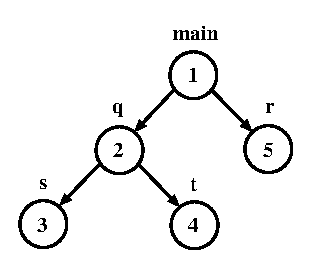
\includegraphics[width=6cm]{fig/pri1-1.eps}
\caption{リダクション順の例}\label{prio1-1}
\end{center}
\end{figure}

非決定性がないこのようなサスペンドしない実行が, 最も効率良いものと言える
\footnote{この例は各述語の引数がないので効率的とも言える.}.  
しかしデータ処理が絡んでくるとそうとも言えない場合がある.  生産者-消費者
の問題を使って次項で説明しよう.  

\subsubsection{過剰生産とその抑制}
非常に単純な次のプログラムを用意する.  

\begin{center}
\begin{minipage}{12cm}\label{gencon}
\begin{Verbatim}[baselinestretch=0.8]
%  gencon.kl1
:- module main.

main:- true |
     generator(100,Stream), consumer(Stream).

generator(0,Stream) :- true | Stream = [].
generator(N,Stream) :- N =\= 0 |
     Stream = [N | NextStream],
     N1 := N - 1,
     generator(N1,NextStream).

consumer([]):- true | true.
consumer([N|Stream]):- integer(N) | consumer(Stream).
\end{Verbatim}
\end{minipage}
\end{center}

このプログラムは図 \ref{prio1-2} の通り整数列が次々に消費者に送られる.  
\begin{figure}[h]
\begin{center}
% \epsfile{file=pri1-2.eps,width=8cm}
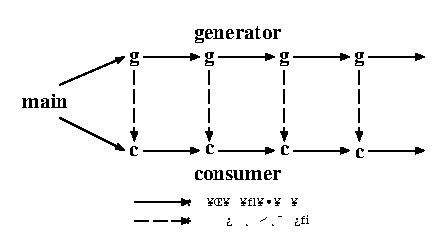
\includegraphics[width=8cm]{fig/pri1-2.eps}
\caption{生産者-消費者問題プログラムの実行}\label{prio1-2}
\end{center}
\end{figure}

前項で取り上げた
LIFO スケジューリングを仮定し, プログラムを実行する.
% \begin{samplebox}
\begin{Verbatim}[frame=single,baselinestretch=0.8]
% klic -o gencon gencon.kl1
% gencon
%
\end{Verbatim}
% \end{samplebox}
無事動いたとしよう.  プログラムを書き換えて生成データを増やす.  
\begin{verbatim}
main :- true | generator(20000,Stream), consumer(Stream).
\end{verbatim}
実行する.  最大ヒープサイズの違いによって次のような実行結果が得られる
可能性がある\footnote{実行時オプション \texttt{-H30k} は, 最大ヒープサイズ
を 30k word として実行することを意味する.}.
% \begin{samplebox}
\begin{Verbatim}[frame=single,baselinestretch=0.8]
% klic -o gencon gencon.kl1
% gencon -H30k
Fatal Error: Maximum heap size specified (30720 words) has been used up
% gencon -H40k
%
\end{Verbatim}
% \end{samplebox}
最大ヒープサイズ 30k ワードで実行するとメモリが足りなくなるのである.  
何故であろうか ?

述語定義を眺めると述語 {\tt generator} が
自分自身をサブゴールとしてリダクションするように記述されている.  
LIFO スケジューリングに従うと仮定すると, 述語{\tt generator} だけ
が次々に走り, 長さ N  のリストを生成して述語 {\tt generator} の
実行が終了する.  次に述語 {\tt consumer} の実行が開始することになる.  
長さ 100 程度の
リストを生産するのは問題なかったが, 長さ 20,000 のリストの生産を試みると
過剰生産でメモリが飽和してしまうことがあり得るのである.  

さてどうするべきか.  ひとつの解決方法として生産者プロセスと
消費者プロセスの間で同期をとる, {\dg 要求駆動的なプログラミング}をする
ことが考えられる.  

\subsubsection{要求駆動型プログラミングによる解決}
次の方針でプログラムを作成する.  
\begin{enumerate}
\item 生産者は生産する必要がなくなったら, その旨を消費者に伝え終了する.  
さもなければ生産者はひとつ整数を消費者に送る.  
\item 消費者は生産終了の旨を受け取ったら終了する.  
消費者は整数をひとつ受け取ったら, 消費した旨を生産者に伝える.  
\item 生産者は消費した旨を受け取ったら上述の手順でさらに生産処理を続ける.  
\end{enumerate}

プログラム例を以下に示す.  
\begin{center}
\begin{minipage}{12cm}
\begin{Verbatim}[baselinestretch=0.8]
%  request.kl1
:- module main.

main :- true | generator(next,20000,Stream), consumer(Stream).

generator(_,0,Stream)    :- true | Stream = [].
generator(Next,N,Stream) :- N =\= 0, Next=next |
     Stream = [send(N,NextN)|NextStream],
     N1 := N - 1,
     generator(NextN,N1,NextStream).

consumer([]) :- true | true.
consumer([send(N,Next)|Stream]) :- integer(N) |
     Next = next,
     consumer(Stream).
\end{Verbatim}
\end{minipage}
\end{center}

さすがにこのプログラムは
% \begin{samplebox}
\begin{Verbatim}[frame=single,baselinestretch=0.8]
% klic -o request request.kl1
% request -H30k
%
\end{Verbatim}
% \end{samplebox}
と, メモリ不足にならずに動く.  

このプログラムは図 \ref{prio1-3} の通り生産者に対して, 
消費者が整数を受け取った後に{\tt next}を送る.  生産者は消費者から
送られてきた{\tt next}で同期をとりながら次の整数を消費者に送る (最初の
 1 回を除く).

実行トレースを見てみよう.  

\begin{figure}[t]
\begin{center}
% \epsfile{file=pri1-3.eps,width=8cm}
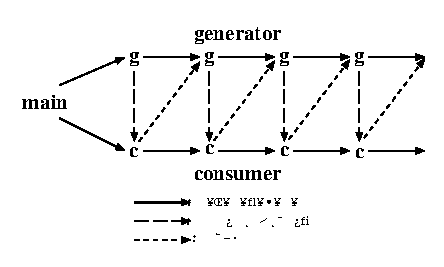
\includegraphics[width=8cm]{fig/pri1-3.eps}
\caption{同期付生産者-消費者問題プログラムの実行}\label{prio1-3}
\end{center}
\end{figure}


% \begin{samplebox}
\begin{Verbatim}[frame=single,baselinestretch=0.8]
   1 CALL: main:main? 
   1 REDU: main:main :-
   2   0:+generator(next,20000,_6)
   3   1:+consumer(_6)? 
   2 CALL: main:generator(next,20000,_6)? 
   2 REDU: main:generator(next,20000,[send(20000,_E)|_F]) :-
   4   0:+generator(_E,19999,_F)? 
   4 CALL: main:generator(_E,19999,_F)? 
   4 SUSP: main:generator(_E,19999,_F)? 
   3 CALL: main:consumer([send(20000,_1B)|_F])? 
   3 REDU: main:consumer([send(20000,next)|_F]) :-
   4   0!+generator(next,19999,_F)
   5   1:+consumer(_F)? 
   4 CALL: main:generator(next,19999,_F)? 
   4 REDU: main:generator(next,19999,_F) :-
   6   0:+generator(next,19999,_F)? 
   6 CALL: main:generator(next,19999,_F)? 
   6 REDU: main:generator(next,19999,[send(19999,_2B)|_2C]) :-
   7   0:+generator(_2B,19998,_2C)? 
   7 CALL: main:generator(_2B,19998,_2C)? 
   7 SUSP: main:generator(_2B,19998,_2C)? 
   5 CALL: main:consumer([send(19999,_38)|_2C])? 
   5 REDU: main:consumer([send(19999,next)|_2C]) :-
   7   0!+generator(next,19998,_2C)
   8   1:+consumer(_2C)? 
   7 CALL: main:generator(next,19998,_2C)? 
   7 REDU: main:generator(next,19998,_2C) :-
   9   0:+generator(next,19998,_2C)? 
   9 CALL: main:generator(next,19998,_2C)? 
   9 REDU: main:generator(next,19998,[send(19998,_48)|_49]) :-
  10   0:+generator(_48,19997,_49)? 
  10 CALL: main:generator(_48,19997,_49)? 
  10 SUSP: main:generator(_48,19997,_49)? a
\end{Verbatim}
% \end{samplebox}
残念ながらサスペンドするゴールが増えていることがわかる.  
要求駆動型にもそれなりの欠点があり, 前項のような
プログラムと併せて時と場合に応じてプログラミングするのが望ましいと
言えよう.  

前項のプログラムを要求駆動型にせずに, KL1 の優先度制御記述を利用して
簡単に実現する方法について次節で説明しよう.  

\section{KL1 のゴール優先度指定方法}
\subsection{再び生産者と消費者の問題}
優先度指定付きのプログラムをまず見せよう.  
\begin{center}
\begin{minipage}{12cm}
\begin{Verbatim}[baselinestretch=0.8]
%  genconwp.kl1
:- module main.

main:- true |
     generator(20000,Stream)@lower_priority, consumer(Stream).

generator(0,Stream) :- true | Stream = [].
generator(N,Stream) :- N =\= 0 |
     Stream = [N | NextStream],
     N1 := N - 1,
     generator(N1,NextStream).

consumer([]):- true | true.
consumer([N|Stream]):- integer(N) | consumer(Stream).
\end{Verbatim}
\end{minipage}
\end{center}

先ほどの要求駆動型プログラムより簡単であり, \pageref{gencon} ページの
プログラムとほとんど変わらない.

次の通りメモリ不足に陥らず, 計算できる.  
% \begin{samplebox}
\begin{Verbatim}[frame=single,baselinestretch=0.8]
% klic -o genconwp genconwp.kl1
% genconwp -H30k
%
\end{Verbatim}
% \end{samplebox}
実行トレースを見てみよう.  
% \begin{samplebox}
\begin{Verbatim}[frame=single,baselinestretch=0.8]
   1 CALL: main:main? 
   1 REDU: main:main :-
   2   0:+consumer(_6)
   3   1*+generator(20000,_6)@prio(67108862)? 
   2 CALL: main:consumer(_6)? 
   2 SUSP: main:consumer(_6)? 
   3 CALL: main:generator(20000,_E)? 
   3 REDU: main:generator(20000,[20000|_14]) :-
   4   0:+generator(19999,_14)
   2   1#+consumer([20000|_14])@prio(67108863)? 
   2 CALL: main:consumer([20000|_14])? 
   2 REDU: main:consumer([20000|_14]) :-
   5   0:+consumer([20000|_14])? 
   5 CALL: main:consumer([20000|_14])? 
   5 REDU: main:consumer([20000|_14]) :-
   6   0:+consumer(_14)? 
   6 CALL: main:consumer(_14)? 
   6 SUSP: main:consumer(_14)? 
   4 CALL: main:generator(19999,_23)? 
   4 REDU: main:generator(19999,[19999|_29]) :-
   7   0:+generator(19998,_29)
   6   1#+consumer([19999|_29])@prio(67108863)? 
   6 CALL: main:consumer([19999|_29])? a
\end{Verbatim}
% \end{samplebox}
実行順序が制御されていることが分かる.  

ソースプログラム中の見慣れない記号を説明しよう.  今までの記述と
異なるのは次の箇所である.  
\begin{center}
\begin{minipage}{12cm}
\begin{verbatim}
generator(20000,Stream)@lower_priority
\end{verbatim}
\end{minipage}
\end{center}

ゴールの後ろについた\verb|@lower_priority|は, {\dg ゴール優先度指定プラグマ}と
呼ばれる.  この記述は{\dg `現在よりひとつ低い優先度でこのゴールリダクションを
試みよ'} を意味する.  この優先度に関しては, 
次の規則に従って KL1 プログラムが実行されている.  
\begin{itemize}
\item ゴール優先度指定プラグマが付いてない限り, サブゴールは親ゴールと同じ優先度となる.  
\end{itemize}
この規則に従うと上述のプログラムは, 次の意味付けされていると
考えることができる.  
\begin{itemize}
\item 消費者は生産者より優先的に実行される.  
\end{itemize}
そんな訳でメモリの大量消費を防ぐことができたのである.  さて文法に
ついて次項で説明しよう.  

\subsection{ゴール優先度指定の文法}

KLIC の優先度は KLIC の整数の表現範囲分だけ存在する.  
大きいほど優先度が高くなる.  

優先度指定の方法は以下の 2 通りある.  
\begin{enumerate}
\item {\dg 絶対指定}

次の通りである.  

\begin{center}
% \begin{samplebox}
\begin{Verbatim}[frame=single]
Goal@priority(優先度)
\end{Verbatim}
% \end{samplebox}
\end{center}

指定されたゴールを指定された優先度でリダクションを試みる.  

\item {\dg 相対指定}

次の通りである.  

\begin{center}
% \begin{samplebox}
\begin{Verbatim}[frame=single]
Goal@lower_priority
\end{Verbatim}
% \end{samplebox}
\end{center}

指定されたゴールの親ゴールより 1 つ低い優先度でリダクションを
試みる.  
\end{enumerate}

\subsection{優先度指定使用上の注意}
優先度指定を使うにあたり, 次のことに注意すべきである.  

\begin{quote}
{\dg 優先度は下げる方向で使うべきである}
\end{quote}

一般的に, 優先度は下げる方向で使うよう心掛けるべきである. 例えば, 
次に示すプログラムは優先度を上げる方向で使った例で, 思った通りには
実行されない悪い優先度の使い方の例である. 


\begin{Verbatim}[baselinestretch=0.8]
        top:- true |
           go@priority(100000)
        go:- true |
           a,b.
        a :- true | goal_0@priority(200000).
        b :- true | goal_1@priority(300000).
\end{Verbatim}

まず, 最低優先度のゴール
{\tt go}の中でゴール{\tt a}と{\tt b}を実行する. それぞれのゴールの
中では, 自分の優先度を 200000 と 300000 に上げている. 
ユーザが意図するところはおそらく次のようなものであろう.

\begin{itemize}
\item ゴール{\tt goal\_0}は優先度 200000 で実行する.
\item ゴール{\tt goal\_1}は優先度 300000 で実行する.
\item すなわち, ゴール{\tt goal\_1}は{\tt goal\_0}より優先的に実行して欲しい.
\end{itemize}

ところが, 実際には次のように実行されて思い通りには動かないかも知れない.

\begin{itemize}
\item ゴール{\tt go}は優先度 100000 で実行される.
\item ゴール{\tt a}と{\tt b}も優先度 100000 で実行される.
\item ゴール{\tt a}が先に実行されて, {\tt goal\_0}が優先度 200000 で実行される.
\item この時点で, ゴール{\tt b}の実行は優先度 100000 で実行されているので, 
優先度 200000 の{\tt goal\_0}の処理が終わるまで, {\tt goal\_1}の実行
は行なわれない.
\end{itemize}

この例の問題点は, ゴールの優先度を変えるという処理を行なうゴール{\tt a}と
{\tt b}の優先度が, 変えた後のゴールの優先度よりも低い点であることは明らかで
あろう. この例はごく単純な例なので, このような間違った優先度制御を行なうことは
まずないと思われるが, プログラム中で動的に優先度を変える場合, しばしば
優先度を上げる方向で使ってしまうことがあるので注意すること.

優先度制御を行なう場合には, あくまでも優先度を下げる方向で使うように心掛け
るべきである.

さらにもうひとつ重要な注意点がある.  次のことである.
\begin{quote}
{\dg ゴール優先度は, 同一プロセッサ内でのみ有効である.}
\end{quote}
マルチプロセッサ環境下で将来 KLIC を動作させる時の注意である.
例えば生産者と消費者を別々のプロセッサで動作させた場合, 
前述のゴール優先度を利用したプログラムでは過剰生産を防ぐことは
できないのである.  

\section{もうひとつの優先度}
ゴールの優先度について述べてきたが, ここではもうひとつの
節優先度指定プラグマ {\bf alternatively} について説明する.  

再度生産者-消費者問題のプログラムを考えてみよう.  今度は
以下プログラムのように生産者が処理を中止するかどうかを判断する
ために変数をひとつもち, この変数に何か値が設定された時に処理を
中止するように定義する. 
\begin{quote}
\begin{Verbatim}[baselinestretch=0.8]
generator(stop,Stream) :- true | Stream = [].
generator(Stop,Stream) :- true |
     Stream = [1 | NextStream],
     generator(Stop,NextStream).
\end{Verbatim}
\end{quote}
説明を簡単にするため整数列を 1 の列で表現した.

このプログラムにはバグがある.  述語 {\tt generator} は 2 つの節をもち, 
次の意味で実行したい.  

\begin{itemize}
\item 第 1 引数に{\tt stop}が到着済みならば, 整数列の生成を止める.  
\item 第 1 引数にまだ{\tt stop}が到着済みでは{\dg ないみたい}ならば, 
整数を 1 つ生成する.  
\end{itemize}

しかしこのプログラムをコンパイルすると

% \begin{samplebox}
\begin{Verbatim}[frame=single,baselinestretch=0.8]
Redundant clause
Clause deleted: generator/2
\end{Verbatim}
% \end{samplebox}

といった警告メッセージが出力される.  
つまりこのままではコンパイラが最適なコードを生成するにあたり, 
述語 {\tt generator} 定義中に冗長節があると指摘してしまう.  
このような場合, リダクションを試行する節に
優先順序を記述することで {\tt generator} 定義にある両節への
リダクションチャンスを与えることができる.  それが {\tt alternatively} である.  
{\tt alternatively} を使ったプログラムを示す.  
\begin{program}
\begin{Verbatim}[baselinestretch=0.8]
generator(stop,Stream) :- true | Stream = [].
alternatively.
generator(Stop,Stream) :- true |
     Stream = [1 | NextStream],
     generator(Stop,NextStream).
\end{Verbatim}
\end{program}
述語{\tt generator}の第 1 節のリダクション, つまり第 1 引数への
メッセージ到着済みであることが確認できれば第 1 節を選択し, 
確認できなければ第 2 節を実行することになる.  
\subsection*{注意点}
次の点を注意すべきである.  
\begin{quote}
{\dg 第 2 節が選択されたからといって, 第 1 引数にメッセージが
到着してないとは限らない.}
\end{quote}
優先度はプログラムの意味を変えないものである.  第 2 節は
第 1 引数が変数でないことを示していないのである.  
KL1 は変数が具体化されたことを確認できるが, 
その逆はできない.  

\section{応用: 幅優先評価の実現}

\begin{figure}
\begin{center}
% \epsfile{file=andor_tree2_exp.eps}\\
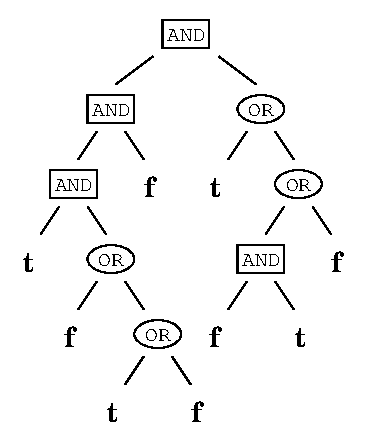
\includegraphics{fig/andor_tree2_exp.eps}\\
and(and(and(t,or(f,or(t,f))),f),or(t,or(and(f,t),f)))
\caption{二進木の例}
\label{andor_tree2_exp}
\end{center}
\end{figure}

ここでは論理式の評価を例にとり, 優先度を用いた幅優先評価の実現方法を述べる.  
一般に, 論理式は, 
AND, OR, t(rue), f(alse) をノードとする二進木で表現することができる.  
例を図\ref{andor_tree2_exp}に示す.  
二進木で表わした場合, 論理式の評価は二進木の評価になる.  

論理式を表わした二進木の評価について, 以下では, まず, 
\begin{itemize}
\item すべてのノードを評価する方法
\item 不要なノード評価を始めない方法
\item 不要なノード評価を打ち切る方法
\end{itemize}
を述べ, そして優先度を用いて
\begin{itemize}
\item 幅優先に評価を行なう方法
\end{itemize}
を述べる.  

\subsection{すべてのノードを評価する方法}

\begin{figure}
\begin{center}
\begin{Verbatim}[baselinestretch=0.8]
% naive.kl1
:- module main.                                                          %  1

main :- true |                                                           %  2
        eval(T,E), io:outstream([print(E),nl]),                          %  3
        T = and(and(and(t,or(f,or(t,f))),f),or(t,or(and(f,t),f))).       %  4

eval(and(L,R),E) :- true | eval(L,EL), eval(R,ER), and_node(EL,ER,E).    %  5
eval(or(L,R),E) :- true | eval(L,EL), eval(R,ER), or_node(EL,ER,E).      %  6
eval(t,E) :- true | E = t.                                               %  7
eval(f,E) :- true | E = f.                                               %  8

and_node(t,t,E) :- true | E = t.                                         %  9
and_node(f,_,E) :- true | E = f.                                         % 10
and_node(_,f,E) :- true | E = f.                                         % 11

or_node(t,_,E) :- true | E = t.                                          % 12
or_node(_,t,E) :- true | E = t.                                          % 13
or_node(f,f,E) :- true | E = f.                                          % 14
\end{Verbatim}
\caption{すべてのノードを評価するプログラム(naive.kl1)}
\label{andor_naive_kl1}
\end{center}
\end{figure}

\begin{figure}
\begin{center}
\begin{Verbatim}[baselinestretch=0.8]
   2 REDU:main:eval(and(and(and(t,or(..)),f),or(t,or(and(..),f))),_3) :-     %  1
   4 REDU:main:eval(and(and(t,or(f,or(..))),f),_F) :-                        %  2
   7 REDU:main:eval(and(t,or(f,or(t,f))),_1C) :-                             %  3
  10 REDU:main:eval(t,t)                                                     %  4
  11 REDU:main:eval(or(f,or(t,f)),_2A) :-                                    %  5
  13 REDU:main:eval(f,f)                                                     %  6
  14 REDU:main:eval(or(t,f),_37) :-                                          %  7
  16 REDU:main:eval(t,t)                                                     %  8
  17 REDU:main:eval(f,f)                                                     %  9
   8 REDU:main:eval(f,f)                                                     % 10
   5 REDU:main:eval(or(t,or(and(f,t),f)),_10) :-                             % 11
  19 REDU:main:eval(t,t)                                                     % 12
  20 REDU:main:eval(or(and(f,t),f),_51) :-                                   % 13
  22 REDU:main:eval(and(f,t),_5D) :-                                         % 14
  25 REDU:main:eval(f,f)                                                     % 15
  26 REDU:main:eval(t,t)                                                     % 16
  23 REDU:main:eval(f,f)                                                     % 17
\end{Verbatim}
\caption{naive.kl1 の実行トレース(eval/2のリダクション)}
\label{andor_naive_log}
\end{center}
\end{figure}

プログラム(naive.kl1)を図\ref{andor_naive_kl1}に示す.  
eval/2は, 下につながるノードがあればeval/2をフォークし, 
フォークによって求まった2つの評価値から自ノードの評価値を決定する(5,6行目).  
下につながるノードのない場合(自分がリーフの場合)は
評価値をすぐに返す(7,8行目).  
and\_node/3及びor\_node/3は2つの値のANDあるいはOR演算を行なう.  

eval/2のリダクションの様子を図\ref{andor_naive_log}に示す.  
このプログラムはすべてのノードを評価してしまうので
図にはすべてのノード(17ノード)が登場した.  


\subsection{不要なノード評価を始めない方法}

\begin{figure}
\begin{center}
\begin{Verbatim}[baselinestretch=0.8]
% seq.kl1
:- module main.                                                          %  1

main :- true |                                                           %  2
        eval(T,E), io:outstream([print(E),nl]),                          %  3
        T = and(and(and(t,or(f,or(t,f))),f),or(t,or(and(f,t),f))).       %  4

eval(and(L,R),E) :- true | eval(L,EL), and_node(EL,R,E).                 %  5
eval(or(L,R),E) :- true | eval(L,EL), or_node(EL,R,E).                   %  6
eval(t,E) :- true | E = t.                                               %  7
eval(f,E) :- true | E = f.                                               %  8

and_node(f,_,E) :- true | E = f.                                         %  9
and_node(t,R,E) :- true | eval(R,E).                                     % 10

or_node(f,R,E) :- true | eval(R,E).                                      % 11
or_node(t,_,E) :- true | E = t.                                          % 12
\end{Verbatim}
\caption{不要なノード評価を始めないプログラム(seq.kl1)}
\label{andor_seq_kl1}
\end{center}
\end{figure}

ANDノードでは, 下につながる2つのノードのうち
一方のノードの評価結果がfならばもう一方のノードは評価する必要がない.  
またORノードでは, 一方がtならばもう一方のノードは評価する必要がない.  
このことを利用して不要なノード評価を行なわくしたのが
図\ref{andor_seq_kl1}のプログラム(seq.kl1)である.  

eval/2は, まずeval/2を呼んで左のノードの評価を行ない, 
and\_node/3あるいはor\_node/3を呼ぶ(5,6行目).  
and\_node/3及びor\_node/3は左のノードの評価結果によって, 
eval/2を呼んで右のノードを評価する(10,11行目), 
あるいは右のノードを評価を始めることなく評価値を返す(9,12行目).  

\begin{figure}[t]
\begin{center}
\begin{Verbatim}[baselinestretch=0.8]
   2 REDU:main:eval(and(and(and(t,or(..)),f),or(t,or(and(..),f))),_3) :-     %  1
   4 REDU:main:eval(and(and(t,or(f,or(..))),f),_F) :-                        %  2
   6 REDU:main:eval(and(t,or(f,or(t,f))),_18) :-                             %  3
   8 REDU:main:eval(t,t)? l                                                  %  4
  10 REDU:main:eval(or(f,or(t,f)),_18) :-                                    %  5
  11 REDU:main:eval(f,f)? l                                                  %  6
  13 REDU:main:eval(or(t,f),_18) :-                                          %  7
  14 REDU:main:eval(t,t)? l                                                  %  8
  16 REDU:main:eval(f,f)? l                                                  %  9

\end{Verbatim}

(a) eval/2のリダクション\\
\vspace{8mm}

% \epsfile{file=andor_tree2_seq.eps}\\

\includegraphics{fig/andor_tree2_seq.eps}\\
(b) ノードの評価
\caption{seq.kl1実行}
\label{andor_seq_log}
\end{center}
\end{figure}

seq.kl1の実行の様子を図\ref{andor_seq_log}に示す.  
不要なノード評価を始めないことにより
17ノード中9ノードについてのみeval/2が実行された.  

このプログラムではnaive.kl1に比べて評価対象のノードが少なくてすむが
(計算量が少なくてすむが)逐次にしか動かない.  
eval/2は2つのゴール(eval/2とand\_node/3あるいはor\_node/3)を
フォークするが(5,6行目), フォークされた2つのゴールは並列には動かない.  
and\_node/3及びor\_node/3はeval/2の結果が求まるまで動けないからである.  


\subsection{不要なノード評価を打ち切る方法}

\begin{figure}
\begin{center}
\begin{Verbatim}[baselinestretch=0.8]
% cont.kl1
:- module main.                                                          %  1

main :- true |                                                           %  2
        eval(_,T,E), io:outstream([print(E),nl]),                        %  3
        T = and(and(and(t,or(f,or(t,f))),f),or(t,or(and(f,t),f))).       %  4

eval(abort,_,_) :- true | true.                                          %  5
alternatively.                                                           %  6
eval(AB,and(L,R),E) :- true |                                            %  7
        and_node(AB,EL,ER,ABL,ABR,E),                                    %  8
        eval(ABL,L,EL), eval(ABR,R,ER).                                  %  9
eval(AB,or(L,R),E) :- true |                                             % 10
        or_node(AB,EL,ER,ABL,ABR,E),                                     % 11
        eval(ABL,L,EL), eval(ABR,R,ER).                                  % 12
eval(_,t,E) :- true | E = t.                                             % 13
eval(_,f,E) :- true | E = f.                                             % 14

and_node(abort,_,_,ABL,ABR,_) :- true | ABL = abort, ABR = abort.        % 15
alternatively.                                                           % 16
and_node(_,t,t,_,_,E) :- true | E = t.                                   % 17
and_node(_,f,_,_,ABR,E) :- true | E = f, ABR = abort.                    % 18
and_node(_,_,f,ABL,_,E) :- true | E = f, ABL = abort.                    % 19

or_node(abort,_,_,ABL,ABR,_) :- true | ABL = abort, ABR = abort.         % 20
alternatively.                                                           % 21
or_node(_,f,f,_,_,E) :- true | E = f.                                    % 22
or_node(_,t,_,_,ABR,E) :- true | E = t, ABR = abort.                     % 23
or_node(_,_,t,ABL,_,E) :- true | E = t, ABL = abort.                     % 24
\end{Verbatim}
\caption{不要なノード評価を打ち切るプログラム(cont.kl1)}
\label{andor_cont_kl1}
\end{center}
\end{figure}

\begin{figure}
\begin{center}
% \epsfile{file=andor_abort.eps}
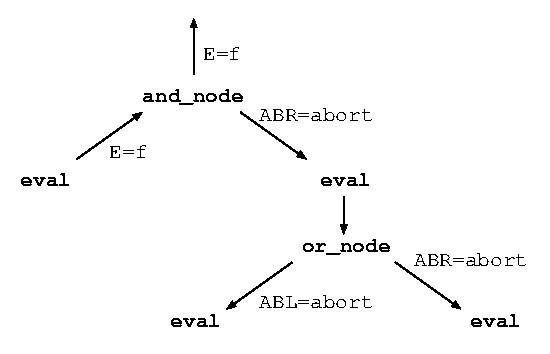
\includegraphics{fig/andor_abort.eps}
\caption{abortの伝播}
\label{andor_abort}
\end{center}
\end{figure}

seq.kl1では不要なノード評価を行なわないことを
\begin{quote}
まず一方のノードを評価し, その結果によってはもう一方の評価を始めない.  
\end{quote}
という逐次的な方式で実現したが, ここでは
\begin{quote}
両方のノードとも評価を始め, たまたま先に求まった一方の評価結果によっては, 
もう一方の評価を途中で打ち切る.  
\end{quote}
という並列実行が可能な方式で実現する.  
この方式では各ノードが並列に評価されうるわけである.  
プログラム(cont.kl1)を図\ref{andor_cont_kl1}に示す.  

eval/3は, 下のノードを評価する2つのeval/3と, 
それらを制御するand\_node/6あるいはor\_node/6をフォークする(7$\sim$12行目).  
フォークされた2つのeval/3は並列に実行されうる.  

eval/3, and\_node/6, or\_node/6 の第1引数は
ノードの評価を途中で打ち切るための引数である.  
この引数を以下では『打ち切り引数』と呼ぶことにする.  
3つの述語とも打ち切り引数をチェックする節(5及び15,20行目)の優先度が
alternativelyによって高くなっている.  
このため打ち切り引数がabortに具体化されていたならば, 
他の引数の具体化状況に依らず打ち切り引数をチェックする節が選択され
ノードの評価は行なわれない.  

and\_node/6は, 
一方のノードの評価結果がfであることがわかった段階で評価値Eをfに決定し, 
打ち切り引数をabortに具体化してもう一方のノードの評価を打ち切る(18,19行目).  
or\_node/6は, 
一方の評価結果がtであることがわかった段階で同様の処理を行なう(23,24行目).  
打ち切り引数の具体化は, and\_nodeあるいはor\_nodeからevalへ, 
そしてand\_nodeあるいはor\_nodeを経由してさらに下のevalへと
伝播して行き(図\ref{andor_abort}参照), ノードの評価が打ち切られる.  

\begin{figure}[t]
\begin{center}
\begin{Verbatim}[baselinestretch=0.8]
   2 REDU:main:eval(_9,and(and(and(t,or(..)),f),or(t,or(and(..),f))),_3) :-  %  1
   5 REDU:main:eval(_16,and(and(t,or(f,or(..))),f),_63E5) :-                 %  2
   8 REDU:main:eval(_30,and(t,or(f,or(t,f))),_63D4) :-                       %  3
  11 REDU:main:eval(_4A,t,t) :-                                              %  4
  12 REDU:main:eval(_45,or(f,or(t,f)),_63C0) :-                              %  5
  15 REDU:main:eval(_6C,f,f) :-                                              %  6
  16 REDU:main:eval(_67,or(t,f),_63AD) :-                                    %  7
  19 REDU:main:eval(_8E,t,t) :-                                              %  8
  20 REDU:main:eval(abort,f,_639C)                                           %  9
   9 REDU:main:eval(_2B,f,f) :-                                              % 10
   6 REDU:main:eval(abort,or(t,or(and(f,t),f)),_63E4)                        % 11

\end{Verbatim}

(a) eval/3のリダクション\\
\vspace{8mm}

% \epsfile{file=andor_tree2_cont.eps}\\
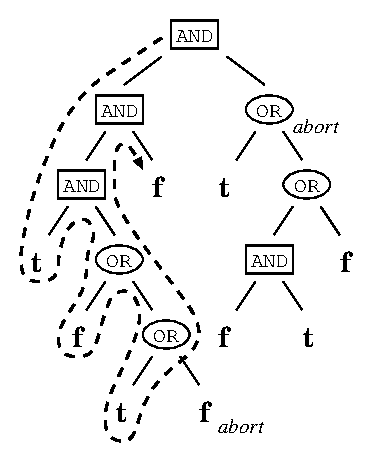
\includegraphics{fig/andor_tree2_cont.eps}\\
(b) ノードの評価
\caption{cont.kl1の実行}
\label{andor_cont_log}
\end{center}
\end{figure}

\begin{figure}
\begin{center}
\begin{Verbatim}[baselinestretch=0.8]
   2 REDU:main:eval(_9,and(and(and(t,or(..)),f),or(t,or(and(..),f))),_3) :-  %  1
   4 REDU:main:eval(_14,and(and(t,or(f,or(..))),f),_12) :-                   %  2
   7 REDU:main:eval(_26,and(t,or(f,or(t,f))),_24) :-                         %  3
  10 REDU:main:eval(_38,t,t)                                                 %  4
  11 REDU:main:eval(_39,or(f,or(t,f)),_37) :-                                %  5
  13 REDU:main:eval(_4A,f,f)                                                 %  6
  14 REDU:main:eval(_4B,or(t,f),_49) :-                                      %  7
  16 REDU:main:eval(_5C,t,t)                                                 %  8
  17 REDU:main:eval(_5D,f,f)                                                 %  9
   8 REDU:main:eval(_27,f,f)                                                 % 10
   5 REDU:main:eval(_15,or(t,or(and(f,t),f)),_13) :-                         % 11
  19 REDU:main:eval(_6E,t,t)                                                 % 12
  20 REDU:main:eval(_6F,or(and(f,t),f),_6D) :-                               % 13
  22 REDU:main:eval(_80,and(f,t),_7E) :-                                     % 14
  25 REDU:main:eval(_92,f,f)                                                 % 15
  26 REDU:main:eval(_93,t,t)                                                 % 16
  23 REDU:main:eval(_81,f,f)                                                 % 17

\end{Verbatim}

(a) eval/3のリダクション\\
\vspace{8mm}

% \epsfile{file=andor_tree2_cont_all.eps}\\

\includegraphics{fig/andor_tree2_cont_all.eps}\\
(b) ノードの評価
\caption{ゴールの順序を入れ換えたcont.kl1の実行}
\label{andor_cont_no_pruning_log}
\end{center}
\end{figure}

cont.kl1の実行の様子を図\ref{andor_cont_log}に示す.  
2つのノードが評価を打ち切られ(図(a) 9,11行目, 図(b) {\it abort\/}), 
17ノード中9ノードについてのみeval/3の通常実行が行なわれた.  
図\ref{andor_cont_log}を図\ref{andor_seq_log}と比較すると
seq.kl1と同じノードが同じ順序で評価されたことがわかる.  
しかしこれは「たまたまそのように評価された」だけである.  
seq.kl1は評価順序を「まず左のノードを評価し, 次に右へ行く」と決めていたが, 
cont.kl1は「どちらもいつでも評価を試みてよい」プログラムであり, 
評価順序は定めていない.  

前述したようにこのプログラムは並列実行が可能である.  
即ち, ある時刻において実行可能なゴールが一般に複数存在する.  
一方このプログラムではゴールに対して優先度を指定していないので
すべてのゴールは同じ優先度をもち実行可能なゴールはどれでも実行されうる.  
これは言い換えると
「あるゴールが実行可能であっても, 一般に, 同じ優先度をもつ実行可能なゴールが
他にも存在するので, そのゴールが実行される保証はない」
ということである.  

評価の打ち切りを効率よく行なうには, 
評価する必要のないノードに対応するeval/3の実行が始まる前に
and\_node/6及びor\_node/6の実行が開始されなければならない.  
実行の終わったeval/3の打ち切り引数を具体化しても意味がないからである.  
しかし, 上述したように, そのように実行される保証はない.  
最悪の場合はすべてのノードについてeval/3の実行が終了してから
and\_node/6及びor\_node/6が実行されノード評価の打ち切りは全く行なわれない.  

図\ref{andor_cont_kl1}のcont.kl1では, 
ボディの左側のゴールが右側より先に実行が試みられたので, 
and\_node/6及びor\_node/6がeval/3よりも先に実行され
ノード評価の打ち切りが行なわれた.  
これは「たまたま期待通りに実行された」と考えるべきである.  
ひとつのボディ内の優先度を指定していないゴール群はすべて同じ優先度を持つので, 
何らかの都合によりeval/3がand\_node/6あるいはor\_node/6より先に実行されても
文句は言えない.  

cont.kl1の8行目と9行目, 及び11行目と12行目を入れ換えると
and\_node/6及びor\_node/6の実行はeval/3の後になる.  
この時のeval/3の実行の様子を図\ref{andor_cont_no_pruning_log}に示す.  
図からわかるようにノード評価の打ち切りは全く行なわれない.  
17ノードすべてについてeval/3が実行されてしまった.  


\subsection{優先度を用いて幅優先に評価を行なう方法}

\begin{figure}
\begin{center}
\begin{Verbatim}[baselinestretch=0.8]
% prio.kl1
:- module main.                                                          %  1

main :- true |                                                           %  2
        eval(_,T,E), io:outstream([print(E),nl]),                        %  3
        T = and(and(and(t,or(f,or(t,f))),f),or(t,or(and(f,t),f))).       %  4

eval(abort,_,_) :- true | true.                                          %  5
alternatively.                                                           %  6
eval(AB,and(L,R),E) :- true |                                            %  7
        and_node(AB,EL,ER,ABL,ABR,E),                                    %  8
        eval(ABL,L,EL)@lower_priority, eval(ABR,R,ER)@lower_priority.    %  9
eval(AB,or(L,R),E) :- true |                                             % 10
        or_node(AB,EL,ER,ABL,ABR,E),                                     % 11
        eval(ABL,L,EL)@lower_priority, eval(ABR,R,ER)@lower_priority.    % 12
eval(_,t,E) :- true | E = t.                                             % 13
eval(_,f,E) :- true | E = f.                                             % 14

and_node(abort,_,_,ABL,ABR,_) :- true | ABL = abort, ABR = abort.        % 15
alternatively.                                                           % 16
and_node(_,t,t,_,_,E) :- true | E = t.                                   % 17
and_node(_,f,_,_,ABR,E) :- true | E = f, ABR = abort.                    % 18
and_node(_,_,f,ABL,_,E) :- true | E = f, ABL = abort.                    % 19

or_node(abort,_,_,ABL,ABR,_) :- true | ABL = abort, ABR = abort.         % 20
alternatively.                                                           % 21
or_node(_,f,f,_,_,E) :- true | E = f.                                    % 22
or_node(_,t,_,_,ABR,E) :- true | E = t, ABR = abort.                     % 23
or_node(_,_,t,ABL,_,E) :- true | E = t, ABL = abort.                     % 24
\end{Verbatim}
\caption{優先度を用いて幅優先評価を行なうプログラム(prio.kl1)}
\label{andor_prio_kl1}
\end{center}
\end{figure}

\begin{figure}
\begin{center}
% \epsfile{file=andor_tree2_prio.eps}
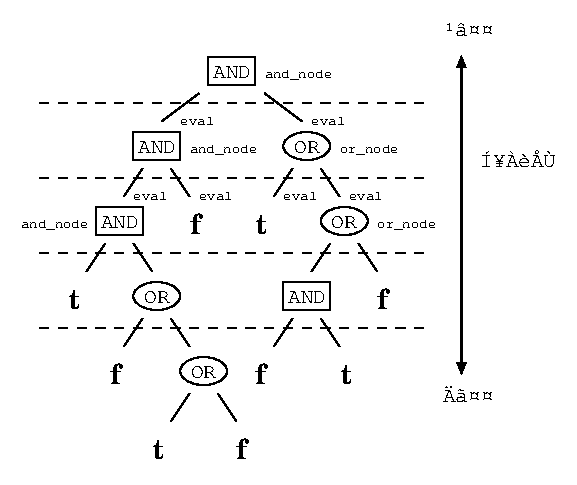
\includegraphics{fig/andor_tree2_prio.eps}
\caption{prio.kl1における優先度}
\label{andor_tree2_prio}
\end{center}
\end{figure}

前述したcont.kl1はゴールの優先度制御を行なわないため
ノード評価打ち切りの機能の働く保証がなかった.  
ここでは優先度を用いて幅優先評価を行ない
ノード評価の打ち切りを行なう方法を示す.  

プログラム(prio.kl1)を図\ref{andor_prio_kl1}に示す.  
このプログラムは9,12行目のeval/3に優先度のプラグマが付いていることを除いて
図\ref{andor_cont_kl1}のcont.kl1と全く同じである.  

eval/3は, 2つのeval/3とand\_node/6あるいはor\_node/6を
フォークするが(7$\sim$12行目), 
2つのeval/3の優先度はand\_node/6及びor\_node/6よりも低い.  
この結果 eval/3よりもand\_node/6及びor\_node/6が優先的に実行され
不要なノード評価の打ち切られることが期待される.  
またルートに近いノードに関するゴールほど高い優先度で実行されるので
全体としては幅優先評価が行なわれる.  

\begin{figure}
\begin{center}
\begin{Verbatim}[baselinestretch=0.8]
   2 REDU:main:eval(_9,and(and(and(t,or(..)),f),or(t,or(and(..),f))),_3) :-  % 1
   6 REDU:main:eval(_11,or(t,or(and(f,t),f)),_63E4) :-                       % 2
   5 REDU:main:eval(_16,and(and(t,or(f,or(..))),f),_63E5) :-                 % 3
  12 REDU:main:eval(_48,f,f) :-                                              % 4
  11 REDU:main:eval(abort,and(t,or(f,or(t,f))),_63C2)                        % 5
   9 REDU:main:eval(abort,or(and(f,t),f),_63D2)                              % 6
   8 REDU:main:eval(abort,t,_63D3)                                           % 7
\end{Verbatim}
\caption{prio.kl1の実行トレース(eval/3のリダクション)}
\label{andor_prio_log}
\end{center}
\end{figure}

図\ref{andor_tree2_prio}にゴールの優先度を, 
図\ref{andor_prio_log}にeval/3のリダクションの様子を示す.  
3つのノードが評価を打ち切られ(5,6,7行目), 
17ノード中4ノードについてのみeval/3の通常実行が行なわれた.  

\section{応用: 簡単な探索問題}

最後に次節に述べる負荷分散制御への理解を深めるために,
非常に良く似た探索問題を優先度制御を利用してプログラム化してみよう.  
探索問題は, 探索木の各ノー
ドを探索して解の含まれているリーフ(葉)を見つける問題である.  探索する
順序には関係なく, 最悪全てのリーフを探索すれば答えは見つかる.  しかし, 
探索問題の多くのものは経験的に木の左の方とか右の方とか, どのあたりに解
が含まれている確率が高いかわかっているものが多い.  ここでは, そのよう
なヒューリスティックを適用できる探索問題を考えてみる.

なお, 同期制御を行なえば木の左から探索するようにプログラムを書く事は可
能であるが, それでは逐次実行しかできない.  ここでは, 並列実行ができか
つヒューリスティックを適用するように, 優先度制御を使ってみよう.


\begin{quote}\begin{dg}\begin{bf}
図\ref{search_tree}に示されるような2分探索木があった時, アトムを含
むリーフを1つ見つけるプログラムを書け.
\end{bf}\end{dg}\end{quote}

\begin{figure}[htb]
        \setlength{\unitlength}{0.9mm}
        \begin{picture}(160,110)(0,0)
        \put(80,100){\framebox(5,5){{\em a}}}
        \put(35,80){\framebox(5,5){{\em b}}}
        \put(125,80){\framebox(5,5){{\em c}}}
        \put(15,60){\framebox(5,5){{\em d}}}
        \put(55,60){\framebox(5,5){{\em e}}}
        \put(105,60){\framebox(5,5){{\em f}}}
        \put(145,60){\framebox(5,5){{\em g}}}
        \put(30,45){\framebox(5,5){{\em h}}}
        \put(90,45){\framebox(5,5){{\em i}}}
        \put(130,45){\framebox(5,5){{\em j}}}
        \put(45,30){\framebox(5,5){{\em k}}}
        \put(105,30){\framebox(5,5){{\em l}}}

        \put(0,45){\makebox(10,5){{\tt 1}}}
        \put(40,45){\makebox(10,5){{\sf here}}}
        \put(67,45){\makebox(10,5){{\sf here}}}
        \put(117,45){\makebox(10,5){{\tt 6}}}
        \put(157,45){\makebox(10,5){{\tt 8}}}
        \put(15,30){\makebox(10,5){{\sf here}}}
        \put(75,30){\makebox(10,5){{\tt 3}}}
        \put(115,30){\makebox(10,5){{\sf here}}}
        \put(145,30){\makebox(10,5){{\tt 7}}}
        \put(30,15){\makebox(10,5){{\tt 2}}}
        \put(60,15){\makebox(10,5){{\sf here}}}
        \put(90,15){\makebox(10,5){{\tt 4}}}
        \put(120,15){\makebox(10,5){{\tt 5}}}

        \put(37.5,85){\line(3,1){45}}
        \put(127.5,85){\line(-3,1){45}}

        \put(17.5,65){\line(4,3){20}}
        \put(57.5,65){\line(-4,3){20}}
        \put(107.5,65){\line(4,3){20}}
        \put(147.5,65){\line(-4,3){20}}
        
        \put(2.5,50){\line(3,2){15}}
        \put(32.5,50){\line(-3,2){15}}
        \put(42.5,50){\line(3,2){15}}
        \put(72.5,50){\line(-3,2){15}}
        \put(92.5,50){\line(3,2){15}}
        \put(122.5,50){\line(-3,2){15}}
        \put(132.5,50){\line(3,2){15}}
        \put(162.5,50){\line(-3,2){15}}

        \put(17.5,35){\line(3,2){15}}
        \put(47.5,35){\line(-3,2){15}}
        \put(77.5,35){\line(3,2){15}}
        \put(107.5,35){\line(-3,2){15}}
        \put(117.5,35){\line(3,2){15}}
        \put(147.5,35){\line(-3,2){15}}

        \put(32.5,20){\line(3,2){15}}
        \put(62.5,20){\line(-3,2){15}}
        \put(92.5,20){\line(3,2){15}}
        \put(122.5,20){\line(-3,2){15}}

        \put(5,47.5){\oval(10,5)}       %1
        \put(45,47.5){\oval(10,5)}      %here
        \put(72,47.5){\oval(10,5)}      %here
        \put(122,47.5){\oval(10,5)}     %6
        \put(162,47.5){\oval(10,5)}     %8
        \put(20,32.5){\oval(10,5)}      %here
        \put(80,32.5){\oval(10,5)}      %3
        \put(120,32.5){\oval(10,5)}     %here
        \put(150,32.5){\oval(10,5)}     %7
        \put(35,17.5){\oval(10,5)}      %2
        \put(65,17.5){\oval(10,5)}      %here
        \put(95,17.5){\oval(10,5)}      %4
        \put(125,17.5){\oval(10,5)}     %5
        \end{picture}
        \caption{探索木}
        \label{search_tree}
\end{figure}


図\ref{search_tree}において四角はノードを表わし, 楕円はリーフを表わす. 
また, ノードには {\em a} から {\em l} の名前が付けてあり, リーフは整数
或いはアトムを値として持つ.  この探索木をここでは次の様なリストデータ
で表わす事にする.
\begin{verbatim}
     [[[1,[here,[2,here]]],[here,here]],[[[3,[4,5]],6],[[here,7],8]]]
\end{verbatim}

ではまず, ヒューリスティクを用いずにこの探索問題を解くプログラムをみて
みよう.  ここでは, アトムが見つかったらそのアトムを要素とするリス
トを返し, 見つからなかったら空リストを返すようにプログラムしてある. 
また, 探索を行なうプロセスは一斉に生成する.  解を一つ見つけたプロセス
は, 探索中の他のプロセスに対してこれ以上探索しなくてもよい旨を通知する. 
なお, 一斉に通知するために全ての探索プロセスは同一の制御用変数を持ち廻
る.  各探索プロセスは, この変数の値が決まるのを alternatively の機能を
使ってチェックする.

%\baselineskip=0.5cm 
\begin{Verbatim}[baselinestretch=0.8]
:- module simple_search.

        search(Tree,Output):- true |               %(1)
                control(Result,Output,Cont),       %(2)
                fork(Tree,Result,Cont).            %(3)
        fork(_,R,stop):-   true | R=[].            %(4)
    alternatively.                                 %(5)
        fork(H,R,Cont):- integer(H) |R=[].         %(6)
        fork(H,R,Cont):- atom(H)    |              %(7)
                R=[H].                             %(8)
        fork([TL,TR],R,Cont):-                     %(9)
                merge:in(R0,R1,R),                 %(10)
                fork(TL,R0,Cont),                  %(11)
                fork(TR,R1,Cont).                  %(12)
        control([H|_],Output,Cont):- wait(H) |     %(13) 
                Output = [H], Cont=stop.           %(14) 
        control([], Output, Cont):- true |         %(15)
                Output = [] .                      %(16) 

:- module merge.

        in([E|In1],In2,Out) :-                     %(17)
                Out = [E|OutT], in(In1,In2,OutT).  %(18)
        in(In1,[E|In2],Out) :-                     %(19)
                Out = [E|OutT], in(In1,In2,OutT).  %(20)
        in([],In2,Out) :-  Out = In2.              %(21)
        in(In1,[],Out) :-  Out = In1.              %(22)

メインプログラム例
:- module main.

        main :-                                    %(23)
           Tree=[[[1,[here,[2,here]]],[here,here]],
                [[[3,[4,5]],6],[[here,7],8]]],
               simple_search:search(Tree,Out),     %(24)
               klicio:klicio([stdout(Result)]),    %(25)
               wait_open(Result, Out).             %(26)
        wait_open(normal(STDOUT), Out) :-          %(27)
           STDOUT=[ putt(Out), nl ].               %(28)
        wait_open(abnormal, _) :- unix:exit(1).    %(29)
\end{Verbatim} 
%\baselineskip=0.8cm

では, プログラムの説明を行なう.

\begin{description}
\item[search]
このプログラムのトップレベルの述語である.  解が 1 つ見つかった時に探索
を終了するための制御を行なうプロセス {\tt control} と探索を行なうプロ
セス {\tt fork} を生成する.
\item[fork]
クローズ (4) では, 変数 {\tt Cont} の値がアトム {\tt stop} に決まった
らそれ以降の探索を中止する.  Alternatively を用いており, このクローズ
は必ず最初に選択される.  {\tt Cont} の値が決まっていなかったら, (6) 以
降のクローズの選択を行なう.
\item[fork]
クローズ (6) では, {\tt H} が整数ならばそれはリーフなのでそれ以上探索
は行なわない.  また, それは解ではないので解を集めるストリームには {\tt
[]} を流す.
\item[fork]
クローズ (8) では, {\tt H} が アトムなら, それはリーフなのでそれ
以上探索は行なわない.  また, それは解なのでストリームにはそのアトム自
身を流す.
\item[fork]
クローズ (9) では, 探索木が 2 要素のリストで各ノードを表わしている場
合に, その左の探索木 {\tt TL} と 右の探索木 {\tt TR}のそれぞれを探索す
るプロセスを (11) と (12) で生成している.  なお, (10) の部分ではここで
生成した2つのプロセスから返ってくる解のストリーム {\tt R0} と {\tt R1} 
をマージインしている.
\item[control]
クローズ (13) では, 解を集めるストリーム {\tt Output} に解が1つでも見
つかった時に, 他の探索を行なうプロセスを中止するために変数 {\tt Cont}
の値を {\tt stop} に決めている.
\item [in]
クローズ (17), (19), (21),(22) で標準的な 2 入力のマージプロセスを
実現している.
\item [main]
クローズ (23) にて計算を行なっている. {\sf [here]} が印刷される.
\end{description}

ここで, {\tt fork} プロセスを生成する部分 (11) と (12) をみてみよう.
(11) はノードの左を探索するプロセスを生成しており, (12) ではノードの右
を探索するプロセスを生成している.  このプログラムを実行すると, もしか
したら右側の探索が優先的に実行され, 例えばノード {\em c} の下の探索ば
かりが実行されるかも知れないが, この下には解が1つしかないので効率は良
くない.

%どのようにこのプログラムに適用すれば
%良いだろうか.  一つは, 同期制御を行なって(13)が終わるまで(14)を実行しない
%ようにする方法である.  しかし, これではせっかくノード {\em b} と {\em c} の
%下の探索は並列に実行させる事が可能なのに, それができなくなる.  

では, 幅優先のヒューリスティクスを, ゴールの優先度制御を用いて
このプログラムに適用してみよう.  優先度を付ける戦略としては, 探索木の
探索するゴール (11) および (12) を呼び出す枝より優先度を低くする.  
すると別の枝の同じ深さのゴールがあった場合は, そちらが優先的に
実行される.

例えば探索ルートの優先度を 4000 とし, このアルゴリズムに従って優先度を
みてみると, 探索木の各ノード及びリーフに
おけるプロセス {\tt fork} の優先度は図\ref{search_tree_priority}のよう
になる.  図中, 各ノード及びリーフの右肩或いは左肩の数字は優先度を表わ
す.  また, 続けてプログラムをみてみよう.

\begin{figure}[htb]
\setlength{\unitlength}{0.9mm}
\begin{picture}(160,110)(0,0)
\put(80,100){\framebox(5,5){{\em a}}}
\put(35,80){\framebox(5,5){{\em b}}}
\put(125,80){\framebox(5,5){{\em c}}}
\put(15,60){\framebox(5,5){{\em d}}}
\put(55,60){\framebox(5,5){{\em e}}}
\put(105,60){\framebox(5,5){{\em f}}}
\put(145,60){\framebox(5,5){{\em g}}}
\put(30,45){\framebox(5,5){{\em h}}}
\put(90,45){\framebox(5,5){{\em i}}}
\put(130,45){\framebox(5,5){{\em j}}}
\put(45,30){\framebox(5,5){{\em k}}}
\put(105,30){\framebox(5,5){{\em l}}}

\put(0,45){\makebox(10,5){{\tt 1}}}
\put(40,45){\makebox(10,5){{\sf here}}}
\put(67,45){\makebox(10,5){{\sf here}}}
\put(117,45){\makebox(10,5){{\tt 6}}}
\put(157,45){\makebox(10,5){{\tt 8}}}
\put(15,30){\makebox(10,5){{\sf here}}}
\put(75,30){\makebox(10,5){{\tt 3}}}
\put(115,30){\makebox(10,5){{\sf here}}}
\put(145,30){\makebox(10,5){{\tt 7}}}
\put(30,15){\makebox(10,5){{\tt 2}}}
\put(60,15){\makebox(10,5){{\sf here}}}
\put(90,15){\makebox(10,5){{\tt 4}}}
\put(120,15){\makebox(10,5){{\tt 5}}}

\put(37.5,85){\line(3,1){45}}
\put(127.5,85){\line(-3,1){45}}

\put(17.5,65){\line(4,3){20}}
\put(57.5,65){\line(-4,3){20}}
\put(107.5,65){\line(4,3){20}}
\put(147.5,65){\line(-4,3){20}}
        
\put(2.5,50){\line(3,2){15}}
\put(32.5,50){\line(-3,2){15}}
\put(42.5,50){\line(3,2){15}}
\put(72.5,50){\line(-3,2){15}}
\put(92.5,50){\line(3,2){15}}
\put(122.5,50){\line(-3,2){15}}
\put(132.5,50){\line(3,2){15}}
\put(162.5,50){\line(-3,2){15}}

\put(17.5,35){\line(3,2){15}}
\put(47.5,35){\line(-3,2){15}}
\put(77.5,35){\line(3,2){15}}
\put(107.5,35){\line(-3,2){15}}
\put(117.5,35){\line(3,2){15}}
\put(147.5,35){\line(-3,2){15}}

\put(32.5,20){\line(3,2){15}}
\put(62.5,20){\line(-3,2){15}}
\put(92.5,20){\line(3,2){15}}
\put(122.5,20){\line(-3,2){15}}

\put(5,47.5){\oval(10,5)} %1
\put(45,47.5){\oval(10,5)} %here
\put(72,47.5){\oval(10,5)} %here
\put(122,47.5){\oval(10,5)} %6
\put(162,47.5){\oval(10,5)} %8
\put(20,32.5){\oval(10,5)} %here
\put(80,32.5){\oval(10,5)} %3
\put(120,32.5){\oval(10,5)} %here
\put(150,32.5){\oval(10,5)} %7
\put(35,17.5){\oval(10,5)} %2
\put(65,17.5){\oval(10,5)} %here
\put(95,17.5){\oval(10,5)} %4
\put(125,17.5){\oval(10,5)} %5

\put(80,105){\makebox(5,5){{\tiny 4000}}}
\put(35,85){\makebox(5,5){{\tiny 3999}}}
\put(125,85){\makebox(5,5){{\tiny 3999}}}
\put(12,65){\makebox(5,5){{\tiny 3998}}}
\put(58,65){\makebox(5,5){{\tiny 3998}}}
\put(102,65){\makebox(5,5){{\tiny 3998}}}
\put(148,65){\makebox(5,5){{\tiny 3998}}}
\put(32,50){\makebox(5,5){{\tiny 3997}}}
\put(87,50){\makebox(5,5){{\tiny 3997}}}
\put(130,50){\makebox(5,5){{\tiny 3997}}}
\put(47,35){\makebox(5,5){{\tiny 3996}}}
\put(106,35){\makebox(5,5){{\tiny 3996}}}

\put(0,50){\makebox(5,5){{\tiny 3997}}}
\put(48,50){\makebox(5,5){{\tiny 3997}}}
\put(71,50){\makebox(5,5){{\tiny 3997}}}
\put(120,50){\makebox(5,5){{\tiny 3997}}}
\put(160,50){\makebox(5,5){{\tiny 3997}}}
\put(23,34){\makebox(5,5){{\tiny 3996}}}
\put(83,34){\makebox(5,5){{\tiny 3996}}}
\put(123,34){\makebox(5,5){{\tiny 3996}}}
\put(150,34){\makebox(5,5){{\tiny 3996}}}
\put(30,20){\makebox(5,5){{\tiny 3995}}}
\put(65,20){\makebox(5,5){{\tiny 3995}}}
\put(90,20){\makebox(5,5){{\tiny 3995}}}
\put(125,20){\makebox(5,5){{\tiny 3995}}}

\end{picture} \caption{探索木の各ノードプロセスの優先度}
\label{search_tree_priority}
\end{figure}


%\baselineskip=0.5cm 
\begin{Verbatim}[baselinestretch=0.8]
:- module search_pri.

        search(Tree,Output):- true |                    %(1)
                control(Results,Output,Cont),           %(2)
                fork(Tree,Results,Cont)@priority(4000). %(3)
        fork(_,R,stop):- true | R=[].                   %(4)
        alternatively.                                  %(5)
        fork(H,R,_):- integer(H) | R=[].                %(6)
        fork(H,R,Cont):- atom(H) |                      %(7)
                R=[H].                                  %(8)
        fork([TL,TR],R,Cont):-true |                    %(9)
                merge:in(R0,R1,R),                      %(10)
                fork(TL,R0,Cont)@lower_priority,        %(11)
                fork(TR,R1,Cont)@lower_priority.        %(12)
        control([H|_],Output,Cont):- wait(H) |          %(13)
                Output=[H], Cont=stop.                  %(14)
        control([],Output,Cont):- true | Output=[].     %(15)

\end{Verbatim} 
%\baselineskip=0.8cm

先のプログラムから変更した部分は, 次の通りである.
\begin{description}
\item {\bf search}\ \ 引数を2つ増やして, 探索を行なうプロセスが使う
最高優先度を指定した.
\item {\bf fork}\ \ (11)と(12)の部分で探索するプロセスを生成する際, 優
先度を下げている.  
\end{description}

なお, この例では探索がある程度以上深くなると優先度はこれ以上低くできな
くなるが, 優先度制御を行なう事によってプログラムは効率的に動く事は分かっ
たであろう.

\section{負荷分散制御の利用目的}

本節では, 負荷分散制御の目的と考え方を説明する.  
一般的に, プログラム中には逐次にしか実行できない部分と
並列に実行できる部分がある.  にも関わらず, 並列に実行できる部分も
逐次計算機では逐次に実行するしか方法がない.  しかし, 
並列計算機では逐次に実行できる部分は同じプロセッサで
実行し, 並列に実行できる部分は別プロセッサで実行でき, 
その点で問題を素直にプログラム化する事ができる.  

KL1では, ボディーゴールの実行はプログラム中に記述した順番とは
全く関係なく実行される.  また, 実行可能な部分は並列に実行される.  
ただし, KLIC 逐次処理系は並列に実行が可能であるとは言っても
プロセッサは1台しかないので, ゴールは同じプロセッサ上で優先度に基づいて
擬似並列的に実行される.  従って, 本当に並列に実行するためには
KLIC 並列処理系上で動かす必要がある.

KL1では, ゴールを別プロセッサで実行させる事を負荷を分散させると呼ぶ.  
負荷を分散させるには, KL1ではプログラム中でそのための指定を
行なう(図\ref{load_distribution}).  
指定の方法についての詳細は次節で説明する.  

\begin{figure}[htb]
        \setlength{\unitlength}{1mm}
        \begin{picture}(150,110)(-10,0)
        \put(0,98){\framebox(35,7)[c]{負荷分散しない場合}}
        \put(80,98){\framebox(35,7)[c]{負荷分散した場合}}

        \put(0, 80){\makebox(30,5)[l]{{\bf a:-true \commit }}}
        \put(5, 75){\makebox(30,5)[l]
                {{\bf Goal$_{1}$,Goal$_{2}$,Goal$_{3}$.}}}
        \put(70,90){\makebox(30,5)[l]{{\bf a:-true \commit }}}
        \put(75,85){\makebox(40,5)[l]
                {{\bf Goal$_{1}$@node(0),}}}
        \put(75,80){\makebox(40,5)[l]
                {{\bf Goal$_{2}$@node(1),}}}
        \put(75,75){\makebox(40,5)[l]
                {{\bf Goal$_{3}$@node(2).}}}
        \put(5,5){\makebox(20,10){{\bf Goal$_{1}$}}}
        \put(5,20){\makebox(20,10){{\bf Goal$_{3}$}}}
        \put(5,35){\makebox(20,10){{\bf Goal$_{2}$}}}
        \put(5,60){\makebox(20,10){{\bf a}}}
        \put(15,60){\vector(0,-1){10}}
        \put(15,35){\vector(0,-1){ 5}}
        \put(15,20){\vector(0,-1){ 5}}
        \put(0,0){\framebox(30,50)[tl]{ノード 0}}
        \put(15,10){\oval(20,10)}
        \put(15,25){\oval(20,10)}
        \put(15,40){\oval(20,10)}
        \put(15,65){\circle{10}}

        \put(40,0){\framebox(30,50)[tl]{ノード 0}}
        \put(80,0){\framebox(30,50)[tl]{ノード 1}}
        \put(120,0){\framebox(30,50)[tl]{ノード 2}}
        \put(55,40){\oval(20,10)}
        \put(95,40){\oval(20,10)}
        \put(135,40){\oval(20,10)}
        \put(95,65){\circle{10}}
        \put(45,35){\makebox(20,10){{\bf Goal$_{1}$}}}
        \put(85,35){\makebox(20,10){{\bf Goal$_{2}$}}}
        \put(125,35){\makebox(20,10){{\bf Goal$_{3}$}}}
        \put(85,60){\makebox(20,10){{\bf a}}}
        \put(95,60){\vector(0,-1){10}}
        \put(95,60){\vector(-4,-1){40}}
        \put(95,60){\vector(4,-1){40}}
        \end{picture}
        \caption{KL1における負荷分散}
        \label{load_distribution}
\end{figure}


負荷分散を行なうにあたっては, プロセスとストリームの構造, 
及び各ゴールの処理の重さ等についてあらかじめ良く考えておく必要がある.  
というのも, 
ゴールの実行を他のノードに依頼するにはそれなりのコストが
必要であり, 並列な部分を全て別ノードに投げれば良いと言うものではない.  

また, 幾ら並列な部分で処理の大きなゴールであっても, 最終的に
莫大なデータを返すようなものであっては, 通信時間のオーバヘッド
が顕著に現れて, 結局全体的には並列効果が現れなくなる場合もある.  

以下に, 負荷分散制御を行なう際に充分気をつけねばならない事項について
まとめてある.  これを参考にして負荷分散制御を行なうと, 並列効果の良い
プログラムを書く指標になる.  


\begin{description}
\item {\bf (1)}{\dg 処理の小さなゴールは負荷分散させない.  \ \ }
幾ら並列性があるとは言っても, 処理の小さなゴールまでも負荷分散させるのは各種の
オーバヘッドによって負荷分散の効果は相殺される.  
ゴールを投げると, {\dg 投げるのに要するコスト}と
{\dg 終了した事を知らせるコスト}が余分にかかる.  これらのコストの和
よりも処理の小さなゴールは, 負荷分散させない方が良い.  
このような処理の小さなゴールを負荷分散するには, 幾つかの関連のある
ゴールをまとめて一つのゴールとし, それを負荷分散する.  

%例えば処理の小さなゴールが1億個あったとしよう.  また, これらは全て
%並列に実行可能で, 一つのゴールの処理にかかるコストが
%1ミリ秒であるとする.  すると, これらを同じプロセッサで逐次に実行すると
%100,000秒かかる.  ここで, 1つのゴールをプロセッサに投げるに要するコスト
%を1ミリ秒だと仮定する.  これらのゴールを単純に100台のプロセッサに
%一つずつ分散させると, 一つのゴールを処理するのに2ミリ秒かかるため, 
%全てのゴールの処理時間は倍の200,000秒かかる.  しかし, 次のように
%負荷を分散させみよう.  
%\begin{enumerate}
%        \item 1億個のゴールを100万個ずつまとめて1つのゴールにする.  
%        \item まとめたゴールを100台のプロセッサに負荷分散する.  
%        \item 各プロセッサは100万個のゴールを逐次処理する.  
%\end{enumerate}
%すると, 負荷分散を行なう回数は100回で済むため, そのためのオーバヘッドは
%100ミリ秒である.  従って, 全体の処理時間は約1,000秒となり, 
%負荷分散の効果は大きい.  

\item {\bf (2)}{\dg なるべくデータのあるノード上で実行させる.  \ \ }
プロセスとデータが所在するノードが異なると, その間の通信の
オーバヘッドが増大する.  プロセスとデータは同じノード上にあるのが
一番望ましい.  各プロセスの処理が充分大きくて別ノードにする方が
効率が良い場合には, 
通信の多いものを同じノード上で処理するようにする事.  


\item {\bf (3)}{\dg アクセスの多いデータベースは, 
ノード毎に分散管理させるのが望ましい.  \ \ }
共通のデータベースを複数のプロセスからアクセスする場合には, 
データベースのあるノードに通信が集中する.  
アクセスの多いデータベースの分割が可能な場合には, できる限り分散管理を
行なって通信が集中しないようにする事.  


\item {\bf (4)}{\dg ゴールについていくデータは
なるべくコンパクトにまとめる.  \ \ }
投げるゴールの実行に必要なデータは, なるべくコンパクトにまとめてられて
いないと通信のオーバヘッドが増大する.  また, その結果も
コンパクトにまとめれている必要がある.  
\end{description}

なお, 今後の研究次第で更に留意する点が次々と出てくるであろう.  
ここでは, 安易に負荷分散を行なうと並列効果を期待できないという
事を良く理解しておき, その基本的な考え方を示した.  

\section{ゴール分散の指定方法}

ゴールの負荷分散の指定は, ボディの各ゴール毎にどのノードで実行するかを
次のようにして指定する.  

\begin{center}
{\bf goal@node(ノード番号)}
\end{center}

なお, ノード番号は0以上の整数であり, ノード数は実行する環境に
より異なる.  そのノード数を得るには次のような組込み述語を用いる.  

\begin{center}
{\bf current\_node(PE,N)}
\end{center}

なお, ここで {\bf PE} はこの組込み述語が実行されたノードの番号で, 
 {\bf N} はノード数のことである.

では, ここで簡単な例を用いて負荷分散の具体的な指定方法を説明しよう.  
次のプログラムは, ゴール {\tt a} をノード 0 と 1 と 2 に投げたもので, 
ノード番号は整数で指定する.  

%\vspace{1.5cm}
%\baselineskip=0.5cm 
\begin{Verbatim}[baselinestretch=0.8]
:- module foo.

        foo:- true |                    %(1)
                a@node(0),              %(2)
                a@node(1),              %(3)
                a@node(2).              %(4)
\end{Verbatim} 
%\baselineskip=0.8cm

また, 変数を用いてノード番号を指定することもできる.  

%\baselineskip=0.5cm 
\begin{Verbatim}[baselinestretch=0.8]
:- module foo.

        foo(P0,P1,P2):- true |          %(1)
                a@node(P0),             %(2)
                a@node(P1),             %(3)
                a@node(P2).             %(4)
\end{Verbatim} 
%\baselineskip=0.8cm

なお, ゴールを別ノードに投げた後には, そのゴールは元と
同じ優先度で実行される.  従って, 例えばノード0で優先度1000
で動いていたゴールはノード1でも優先度1000で実行される.  
その時ノード0では優先度1000以上のゴールがなかった場合には, 
このゴールはノード1では直ちに実行される.  しかし, 投げた先のノード1では
優先度2000のゴールが忙しく実行されているかも知れない.  その場合, 
投げられたゴールはすぐには実行されない.  優先度制御を行なっている場合には, 
このようなことが起こり得るということを覚えておこう.  

なお, ノードの割り付け方法には色々あるが, 幾つかの代表的なものを
例にして, 負荷分散制御の方法を実際のプログラムでみてみよう.  

\subsection*{サイクリック割り付け}
ノード数 4 の構成でゴール{\tt spawn}のプロセスを 8 個サイクリックに
割り付けたプログラム例を次に示す.   生成するプロセスの
個数は引数で指定し, ノード数も組込み述語で調べているため, 
汎用的に使える例である.  

%\baselineskip=0.5cm 
\begin{Verbatim}[baselinestretch=0.8]
:- module foo.
        distribute(N):- true |                  %(1)
                current_node(_,PEs),            %(2)
                fork(N,PEs,0).                  %(3)
        fork(0,PEs,PE):- true | true.           %(4)
        otherwise.
        fork(N,PEs,PE):- PeNo:=PE mod PEs|      %(5)
                spawn@node(PeNo),               %(6)
                NextPE:=PE+1,                   %(7)
                N1:=N-1,                        %(8)
                fork(N1,PEs,NextPE).            %(9)

\end{Verbatim} 
%\baselineskip=0.8cm

``\verb|foo:distribute(8)|'' を実行すると, {\tt spawn}プロセスはノード
の 0, 1, 2, 3, 0, 1, 2, 3 に割り付けられる.  

\subsection*{ランダム割り付け}

ノードをサイクリックに割り付けると, 規則性のあるプログラムでは
特定のノードに負荷が集中してしまう場合がある.  それを回避する一つの
割り付け手法がランダム割り付けである.  割り付けるノードの番号を
乱数によって決める手法である.  次に示したプログラムは{\tt spawn}
プロセスを 100 個擬似乱数を使ってノードに割り付けた例である.  

%\baselineskip=0.5cm 
\begin{Verbatim}[baselinestretch=0.8]
:- module foo.

        distribute(N):- true |                  %(1)
                current_node(_,PEs),            %(2)
                random(Rs,23,PEs),              %(3)
                fork(N,Rs).                     %(4)
        fork(0,Rs):- true | Rs=[].              %(5)
     otherwise.
        fork(N,Rs):- true |                     %(6)
                Rs=[get(PeNo)|NewRs],           %(7)
                spawn@node(PeNo),               %(8)
                N1:=N-1,                        %(9)
                fork(N1,NewRs).                 %(10)
        random([get(Rnd)|RS],Seed,R):- true |   %(11)
                Rnd:= Seed mod R,               %(12)
                NewSeed:=(125*Seed+1) mod 4096, %(13)
                random(RS,NewSeed,R).           %(14)
        random([],_,_):- true | true.           %(15)

\end{Verbatim} 
%\baselineskip=0.8cm

(16)のようにゴールを呼び出すと, 100 ノードの環境であれば, 
(7)の部分で乱数生成プロセスから0から99までの一様乱数を得, 
(8)の部分でノードの割り付けを行なう.  
この例の場合では, ノードは 23, 76, 49, 10, 99, 32, $\cdots$ と
割り付けられる.  

\subsection*{暇なノードへの動的割り付け}

この方式は, 暇なノードが誰であるかを OS なり処理系なりに尋ねて, ゴール
を投げようとした時に一番暇だと思われるノードに割り付ける方式である. 
ただし, 残念ながらこのような機能はないので,
本格的に動的割り付けを行なうのは今後の研究成果に期待しよう.  

しかし, 処理系の機能を使わなくても似た機能を実現することはできる.  
まず, 単純なカウンタゴール\footnote{再帰呼び出しを使ってループした回数を
カウントするゴール}を用意する.  
また, あるノードには全ノードのカウンタ値を管理する
マネージャゴールを用意し, これに最高優先度を与える.  
次に, 全てのノードにカウンタゴールを
投げ, それにシステムの最低優先度を与える.  即ち, 各ノードは他に
何も実行するゴールがなくなった時にこのカウンタゴールを実行する.  
カウンタゴールは, 一定時間おきに自分のカウンタ値をマネージャに通知する.  
もし, ノードが忙しければ小さなカウント値がマネージャには通知される.  
或いは, 忙し過ぎて通知が遅れるかも知れない.  また, ノードが暇であれば
大きなカウント値が通知される.  
マネージャゴールには最高優先度が与えられているので, 各ノードから
カウント値が通知されれば直ちにそれを集める事ができる.  
このマネージャに対して問い合わせすれば, 
カウント値を元にして, どのノードが暇であるかが大体わかる.  

このようにして暇そうなノードを見つけることは可能であるが, 
一般的に本当に暇なノードを見つけるのは難しい.  
例えば, 処理系に尋ねた瞬間には本当に暇であっても, そのノードにゴールを投げて
それが到着した時には実は大変忙しいかも知れない.  このような動的な
負荷分散の方式は並列計算機一般の現在の研究課題であり, 興味のある人は
是非トライしてみる価値があるだろう.  


\section{応用: 簡単な探索問題}

本節では, 負荷分散制御を応用したプログラム例を示す.  ここで示すプ
ログラム及び負荷分散アルゴリズムは一例である.  各自でプログラムを書き
換えたり, また負荷分散アルゴリズムを変えて色々評価をしてみると大変よい
と思う.

\subsection*{簡単な探索問題}
ゴールの優先度を勉強した際に用いた簡単な探索問題プログラムに, 今度は更
に負荷分散制御を応用してみよう.  プログラムは先に用いたものを拡張し, 
負荷分散アルゴリズムはサイクリック割り付けを用いる.

また, 負荷分散は探索木が別れる部分で行なう.  ただし, あまり細かく分散
すると負荷分散のためのオーバヘッドが増大するので, 探索がある程度のレベ
ル(この例の場合は2)に達するまでは同じノードで実行し, レベルに達したと
ころでサイクリックにノード割り付けを行なって負荷分散する.  この探索木
は2分木なので, 探索レベル3のところ兄弟の数は$2^{3}$個になり, 8台のノー
ドに負荷分散する事になる.

なお, 負荷分散した先ではそれ以上の負荷分散は行なわず, 優先度制御のみを
行なう.  この例では, 先に用いた {\tt search\_pri} モジュール (
\pageref{search_tree_priority} ページ参照) のゴールを
ただ呼び出しているだけである.  また, ノードの番号を得るためのサーバプ
ロセスを設け, 負荷分散を行なう前にはこのプロセスに対してノード番号を問
い合わせるものとする.

では, まず図\ref{search_tree_distribution}に各ノードのプロセスがどのノー
ドで実行されるかを示す.  また, 各ノード内での優先度も示す.  図中, 各ノー
ド及びリーフの右肩或いは左肩の数字は優先度を表わす.  また, 右或いは左
の数字は実行されるノードを表わす.  続けてプログラムをみてみよう.

\begin{figure}[htb]
\setlength{\unitlength}{0.9mm}
\begin{picture}(160,110)(0,0)
\put(80,100){\framebox(5,5){{\em a}}}
\put(35,80){\framebox(5,5){{\em b}}}
\put(125,80){\framebox(5,5){{\em c}}}
\put(15,60){\framebox(5,5){{\em d}}}
\put(55,60){\framebox(5,5){{\em e}}}
\put(105,60){\framebox(5,5){{\em f}}}
\put(145,60){\framebox(5,5){{\em g}}}
\put(30,45){\framebox(5,5){{\em h}}}
\put(90,45){\framebox(5,5){{\em i}}}
\put(130,45){\framebox(5,5){{\em j}}}
\put(45,30){\framebox(5,5){{\em k}}}
\put(105,30){\framebox(5,5){{\em l}}}

\put(0,45){\makebox(10,5){{\tt 1}}}
\put(40,45){\makebox(10,5){{\sf here}}}
\put(67,45){\makebox(10,5){{\sf here}}}
\put(117,45){\makebox(10,5){{\tt 6}}}
\put(157,45){\makebox(10,5){{\tt 8}}}
\put(15,30){\makebox(10,5){{\sf here}}}
\put(75,30){\makebox(10,5){{\tt 3}}}
\put(115,30){\makebox(10,5){{\sf here}}}
\put(145,30){\makebox(10,5){{\tt 7}}}
\put(30,15){\makebox(10,5){{\tt 2}}}
\put(60,15){\makebox(10,5){{\sf here}}}
\put(90,15){\makebox(10,5){{\tt 4}}}
\put(120,15){\makebox(10,5){{\tt 5}}}

\put(37.5,85){\line(3,1){45}}
\put(127.5,85){\line(-3,1){45}}

\put(17.5,65){\line(4,3){20}}
\put(57.5,65){\line(-4,3){20}}
\put(107.5,65){\line(4,3){20}}
\put(147.5,65){\line(-4,3){20}}
        
\put(2.5,50){\line(3,2){15}}
\put(32.5,50){\line(-3,2){15}}
\put(42.5,50){\line(3,2){15}}
\put(72.5,50){\line(-3,2){15}}
\put(92.5,50){\line(3,2){15}}
\put(122.5,50){\line(-3,2){15}}
\put(132.5,50){\line(3,2){15}}
\put(162.5,50){\line(-3,2){15}}

\put(17.5,35){\line(3,2){15}}
\put(47.5,35){\line(-3,2){15}}
\put(77.5,35){\line(3,2){15}}
\put(107.5,35){\line(-3,2){15}}
\put(117.5,35){\line(3,2){15}}
\put(147.5,35){\line(-3,2){15}}

\put(32.5,20){\line(3,2){15}}
\put(62.5,20){\line(-3,2){15}}
\put(92.5,20){\line(3,2){15}}
\put(122.5,20){\line(-3,2){15}}

\put(5,47.5){\oval(10,5)} %1
\put(45,47.5){\oval(10,5)} %here
\put(72,47.5){\oval(10,5)} %here
\put(122,47.5){\oval(10,5)} %6
\put(162,47.5){\oval(10,5)} %8
\put(20,32.5){\oval(10,5)} %here
\put(80,32.5){\oval(10,5)} %3
\put(120,32.5){\oval(10,5)} %here
\put(150,32.5){\oval(10,5)} %7
\put(35,17.5){\oval(10,5)} %2
\put(65,17.5){\oval(10,5)} %here
\put(95,17.5){\oval(10,5)} %4
\put(125,17.5){\oval(10,5)} %5

\put(80,105){\makebox(5,5){{\tiny 4000}}}
\put(35,85){\makebox(5,5){{\tiny 4000}}}
\put(125,85){\makebox(5,5){{\tiny 4000}}}
\put(12,65){\makebox(5,5){{\tiny 4000}}}
\put(58,65){\makebox(5,5){{\tiny 4000}}}
\put(102,65){\makebox(5,5){{\tiny 4000}}}
\put(148,65){\makebox(5,5){{\tiny 4000}}}

\put(32,50){\makebox(5,5){{\tiny 4000}}}
\put(87,50){\makebox(5,5){{\tiny 4000}}}
\put(130,50){\makebox(5,5){{\tiny 4000}}}
\put(47,35){\makebox(5,5){{\tiny 3999}}}
\put(106,35){\makebox(5,5){{\tiny 3999}}}

\put(0,50){\makebox(5,5){{\tiny 4000}}}
\put(48,50){\makebox(5,5){{\tiny 4000}}}
\put(71,50){\makebox(5,5){{\tiny 4000}}}
\put(120,50){\makebox(5,5){{\tiny 4000}}}
\put(160,50){\makebox(5,5){{\tiny 4000}}}
\put(23,34){\makebox(5,5){{\tiny 3999}}}
\put(83,34){\makebox(5,5){{\tiny 3999}}}
\put(123,34){\makebox(5,5){{\tiny 3999}}}
\put(150,34){\makebox(5,5){{\tiny 3999}}}
\put(30,20){\makebox(5,5){{\tiny 3998}}}
\put(65,20){\makebox(5,5){{\tiny 3998}}}
\put(90,20){\makebox(5,5){{\tiny 3998}}}
\put(125,20){\makebox(5,5){{\tiny 3998}}}
\put(85,100){\makebox(5,5){{\tt 0}}}
\put(40,80){\makebox(5,5){{\tt 0}}}
\put(130,80){\makebox(5,5){{\tt 0}}}
\put(20,60){\makebox(5,5){{\tt 0}}}
\put(60,60){\makebox(5,5){{\tt 0}}}
\put(110,60){\makebox(5,5){{\tt 0}}}
\put(150,60){\makebox(5,5){{\tt 0}}}
\put(35,45){\makebox(5,5){{\tt 1}}}
\put(95,45){\makebox(5,5){{\tt 4}}}
\put(135,45){\makebox(5,5){{\tt 6}}}
\put(50,30){\makebox(5,5){{\tt 1}}}
\put(110,30){\makebox(5,5){{\tt 4}}}

\put(10,45){\makebox(5,5){{\tt 0}}}
\put(50,45){\makebox(5,5){{\tt 2}}}
\put(77,45){\makebox(5,5){{\tt 3}}}
\put(113,45){\makebox(5,5){{\tt 5}}}
\put(167,45){\makebox(5,5){{\tt 7}}}
\put(25,30){\makebox(5,5){{\tt 1}}}
\put(85,30){\makebox(5,5){{\tt 4}}}
\put(125,30){\makebox(5,5){{\tt 6}}}
\put(155,30){\makebox(5,5){{\tt 6}}}
\put(40,15){\makebox(5,5){{\tt 1}}}
\put(70,15){\makebox(5,5){{\tt 1}}}
\put(100,15){\makebox(5,5){{\tt 4}}}
\put(130,15){\makebox(5,5){{\tt 4}}}

\end{picture}
\caption{探索木の各ノードプロセスの実行されるノードと優先度}
\label{search_tree_distribution}
\end{figure}

%\baselineskip=0.5cm 
\begin{Verbatim}[baselinestretch=0.8]
:- module search_load_balancing.

        search(Tree,Output):- true |                    %(1)
                current_node(PE,PEs),                   %(2)
                control(Results,Output,Cont),           %(3)
                fork(Tree,Results,0,PeServer,Cont)
                             @priority(4000),           %(4)
                next_pe(PeServer,PE,PEs).               %(5)
        fork(_,R,_,Next,stop):- true | R=[], Next=[].   %(6)
        alternatively.                                  %(7)
        fork(H,R,_,Next,_):- integer(H) |               %(8)
                R=[], Next=[].                          %(9)
        fork(H,R,_,Next,Cont):- atom(H) |               %(10)
                R=[H], Next=[].                         %(11)
        fork([TL,TR],R,Level,Next,Cont):-               %(12)
                Level =< 1 |                            %(13)
                L1 := Level+1,                          %(14)
                merge:in(R0,R1,R),                      %(15)
                merge:in(Next0,Next1,Next),             %(16)
                fork(TL,R0,L1,Next0,Cont),              %(17)
                fork(TR,R1,L1,Next1,Cont).              %(18)
        fork([TL,TR],R,Level,Next,Cont):-               %(19)
                Level =:= 2 |                           %(20)
                Next=[get(PE0),get(PE1)],               %(21)
                merge:in(R0,R1,R),                      %(22)
                search_pri:fork(TL,R0,Cont)@node(PE0),  %(23)
                search_pri:fork(TR,R1,Cont)@node(PE1).  %(24)

        control([H|_],Output,Cont):- wait(H) |          %(25)
                Output=[H], Cont=stop.                  %(26)
        control([],Output,Cont):- true | Output=[].     %(27)
        
        next_pe([],_,_):- true | true .                 %(28)
        next_pe([get(PeNo)|Next],PE,PEs):-true |        %(29)
                PE1 := PE+1,                            %(30)
                PeNo := PE mod PEs,                     %(31)
                next_pe(Next,PE1,PEs).                  %(32)
\end{Verbatim} 
%\baselineskip=0.8cm

\begin{description}
\item {\bf search}\ \ このプログラムを呼び出すトップレベルの述語である.  
引数は先の例と全く同じである.  ボディゴールでは, まず組込み述語で自分
のノード番号と全体のノード数を計算している(2). (3), (4)では探索を行な
うプロセスを生成している.  (5)ではノード番号を得るサーパプロセスを生成
している.
\item {\bf fork\ クローズ(12)}\ \ 探索のレベルが1以下の時には同じノードで
実行する.  なお, ここで (17), (18) の優先度を変えていないが, これは負
荷分散作業を最優先で実行するためである.  即ち, 優先度を下げると探索作
業と負荷分散作業が並行して行なわれ, ノードに投げる処理が遅れるからであ
る.
\begin{quote}\begin{dg}
負荷分散が完了するまでは, 負荷分散作業を行なうゴールのプライオリティは
他のゴールのプライオリティよりも低くならないようにするように注意しなけ
ればならない.
\end{dg}\end{quote}
\item {\bf fork\ クローズ(19)}\ \  探索のレベルが 2 に達した時, 
左右の探索を別ノードで実行させるようゴールを投げている (23), (24).  い
ずれのゴールも, 実行する優先度の範囲はトップレベルのゴール呼び出しで与
えられた引数をそのまま渡している.  \\ここで {\tt \ search\_pri:\ \ } 
の後にゴールを記述しているが, これは別モジュールのゴールを呼び出すため
の表記である.  優先度制御は, このモジュール の中で行なわれる.  なお,
(21) の部分で動作させるべきノード番号を得ている.
\item {\bf next\_pe}\ \ ノード番号をサイクリックに得るためのサーバである.  
\end{description}

\clearpage

\exercise{二進木の探索}

二進木を幅優先に探索するプログラムを書け.  
二進木の形式を図\ref{exp_tree2}に示す.  

リーフがアトムならばそれが解であり, 
整数ならばそこには解がないものとする.  
解が求まったら解に至るルートを[left,right,...,アトム名]の形式で表示する.  
例えば図\ref{exp_tree2}の例でアトムa が見つかった場合は [left,right,left,a] と
表示する.  
例として以下の二進木T について実行してみよ.  
\begin{quote}\begin{quote}
\begin{Verbatim}[baselinestretch=0.8]
T = n(n(n(n(1,n(2,3)),n(4,n(n(a,5),6))),n(b,7)),
      n(n(n(8,n(9,c)),10),n(n(d,11),12))).  
\end{Verbatim}
\end{quote}\end{quote}

\begin{figure}[h]
\begin{center}
% \epsfile{file=exp_tree2.eps}\\
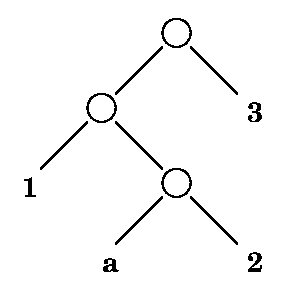
\includegraphics{fig/exp_tree2.eps}\\
n(n(1,n(a,2)),3)
\caption{二進木の形式}
\label{exp_tree2}
\end{center}
\end{figure}

\chapter{総合演習問題}
\exercise{ストリームの要素を除去するプログラム}
与えられたストリームから指定された要素を全て除去したストリームを作るプ
ログラムを作成しなさい. 例えば, ストリームとして \verb|[1,2,1,3,1]| を
与え, 除去する要素を \verb|1| とすると, 結果として \verb|[2,3]| が返
る(図 \ref{remove}). 

なお, KL1 のアトミックな項 \verb|A| と \verb|B| が等しくないことを調べ
るには, ガード部で ``\verb|A \= B|'' を実行すればよい. または,
``\verb|\=|'' の代わりに ``\verb|otherwise|'' を用いてもよい. 

\begin{figure}[h]
\begin{center}
\unitlength\columnwidth
\divide\unitlength 1700
\begin{picture}(1200,300)
\put(500,0){\framebox(200,300){remove}}
\put(200,200){\line(1,0){300}}
\put(200,100){\line(1,0){300}}
\put(700,200){\line(1,0){300}}
\put(700,100){\line(1,0){300}}
\put(350,150){\makebox(0,0){1,3,1,2,1 $\rightarrow$}}
\put(850,150){\makebox(0,0){3,2 $\rightarrow$}}
\end{picture}
\end{center}

\caption{ストリームの要素の除去}
\label{remove}
\end{figure}

\exercise{ストリームを圧縮するプログラム}
与えられたストリームから同一要素をすべて除去したストリームを作るプログ
ラムを作成しなさい. 例えば, ストリームとして 
\verb|[1,2,3,4,5,4,3,2,1]| を与えると, 結果として \verb|[1,2,3,4,5]| 
が返る(図 \ref{compact}).  

なお, ストリームから要素を除去するには, 前の問題で作成したプログラムを
利用するとよい. 

\begin{figure}[h]
\begin{center}
\unitlength\columnwidth
\divide\unitlength 1700
\begin{picture}(1200,300)
\put(500,0){\framebox(200,300){compact}}
\put(200,200){\line(1,0){300}}
\put(200,100){\line(1,0){300}}
\put(700,200){\line(1,0){300}}
\put(700,100){\line(1,0){300}}
\put(300,150){\makebox(0,0){1,2,3,4,5,4,3,2,1 $\rightarrow$}}
\put(850,150){\makebox(0,0){5,4,3,2,1 $\rightarrow$}}
\end{picture}
\end{center}

\caption{ストリームの圧縮}
\label{compact}
\end{figure}

\newpage

\exercise{1,000 以下の素数列を生成するプログラム}\label{q1}
1,000 以下の素数を生成し, 生成させた素数の個数を数えて
表示するプログラムを作成しなさい.

\begin{description}
\item [ヒント] 図 \ref{qans1}, 図 \ref{qans2} のプロセス構造を参考にせよ.  
素数フィルタは, 新しい素数がみつかった度に生成される.
\end{description}

\begin{figure}[h]
\begin{center}
% \epsfile{file=ans11.eps,width=10cm}
\includegraphics[width=9.5cm]{fig/ans11.eps}
\caption{プロセス初期状態}\label{qans1}
\end{center}
\end{figure}

\begin{figure}[h]
\begin{center}
% \epsfile{file=ans12.eps,width=10cm}
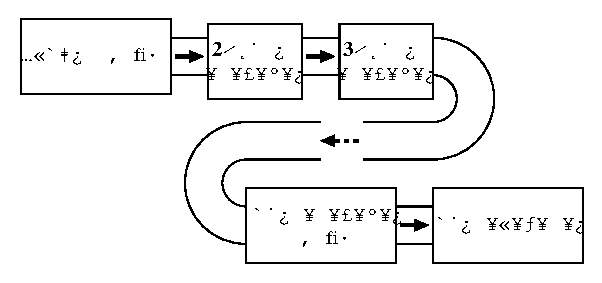
\includegraphics[width=9cm]{fig/ans12.eps}
\caption{プログラム実行中}\label{qans2}
\end{center}
\end{figure}

\newpage

\exercise{20,000 以下の素数列を生成するプログラム}
20,000 以下の素数を生成し, 生成させた素数の個数を数えて
表示するプログラムを作成しなさい.

\begin{description}
\item [ヒント] 前問と同様な方法を用いると自然数生成器が
走り過ぎメモリを大量に消費してしまう.  このことを防ぐために要求駆動的な
プロセス構造を設定する.  図 \ref{qans3} のプロセス構造を参考にせよ.  
同期をとる方法は次の通り.  自然数生成器は自然数生成単位
 (例えば 100 個毎) にすべての素数フィルタを通りなおかつフィルタ
プロセスを生成しないデータをひとつ送り, そしてカウンタから
次の生成要求が送られてくるのを待つ.  
カウンタはこのデータを受け取った後, 次のデータ生成要求を
自然数生成器に送る.  自然数生成器は, データ生成要求に従い次の
自然数列を生成する.
\end{description}

\begin{figure}[h]
\begin{center}
% \epsfile{file=ans13.eps,width=10cm}
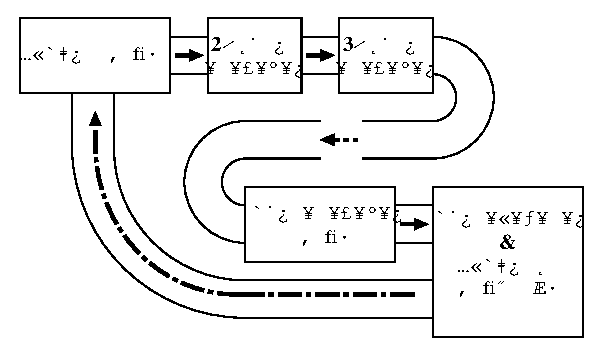
\includegraphics[width=9cm]{fig/ans13.eps}
\caption{同期機構付きプロセス構造}\label{qans3}
\end{center}
\end{figure}

\vspace{0.5cm}

もちろん優先度制御を用いるプログラムもある.


\exercise{1,000 番目の素数を求めるプログラム}
小さい方から数えて 1,000 番目の素数を求め, それを表示するプログラムを
作成しなさい. 

\appendix
\setcounter{exercise}{0}
\chapter{演習問題の解答例}

\answer{フィボナッチ数の平方と立方の総和}
データ駆動で書いたものが次のプログラムである.  
本文中に出てきた fibonacci/4, square/2, cube/2 merge/3 sum/2を
ストリームでつなげば良い.  

%\begin{program}
\begin{Verbatim}[baselinestretch=0.8]
        :- module main.

        main :- true|
            main(100,Answer),
            io:outstream([print(Answer),nl]).

        main(Target,Answer) :- true|
            fibonacci(0,1,Fibo,Target),
            square(Fibo,Squares), cube(Fibo,Cubes),
            merge(Squares,Cubes,Both),
            sum(Both,Answer).
\end{Verbatim}
%\end{program}

\verb!Target!=100とした時の答えは, 935596である.  

要求駆動, あるいはメッセージ駆動で書くのなら, 
フィボナッチプロセスに要求を出し, その結果であるフィボナッチ数を
square/2, cube/2 で実現されるフィルタプロセスに配るプロセスを
組み込むのが良い.  
以下のプログラムはメッセージ駆動で書いたものである.  
square/2, cube/2, merge/3, sum/2は本文中と同じである.  

%\begin{program}
\begin{Verbatim}[baselinestretch=0.8]
        :- module main.

        main :- true|
            main(100,Answer),
            io:outstream([print(Answer),nl]).

        main(Target,Answer) :- true|
            fibonacci_lazy(0,1,Stream),
            dispatch(Stream,Target,Fibo),
            square(Fibo,Squares), cube(Fibo,Cubes),
            merge(Squares,Cubes,Both),
            sum(Both,Answer).

        fibonacci_lazy(N1,N2,[]) :- true | true.
        fibonacci_lazy(N1,N2,[make(X)|Stream]) :- true|
            X = N2,
            N3 := N1 + N2,
            fibonacci_lazy(N2,N3,Stream).

        dispatch(Stream,Target,Fibo) :- true | 
            Stream = [make(X)|StreamN],
            dispatch(StreamN,Target,Fibo,X).

        dispatch(Stream,Target,Fibo,X) :- X >= Target|
            Stream = [],
            Fibo = [].
        dispatch(Stream,Target,Fibo,X) :- X < Target|
            Fibo = [X|FiboN],
            dispatch(Stream,Target,FiboN).
\end{Verbatim}

\answer{$2^{l} \times 3^{m} \times 5^{n}$}
入力を正の整数\verb!N!で割れるだけ割った数を出力するフィルタを用意する.  
例えば, \verb!N!=2 としたものに12を通すと3を出力するようなフィルタである.  
また, 入力のうち1が何個あったかをカウントするカウンタプロセスを用意する. 
そして, 
\verb!N!=2としたフィルタ, \verb!N!=3としたフィルタ, \verb!N!=5としたフィルタ, 
これらをつないだパイプラインの前に自然数生成プロセス, 
後ろにカウンタプロセスをつないで, 図~\ref{pipe_line}のような
プロセス・ネットワークを作れば, 問題の式で表せる数が幾つあるかを
計算するプロセス・ネットワークが出来る.  

\begin{figure}
\begin{center}
% \epsfile{file=pipeline.eps}
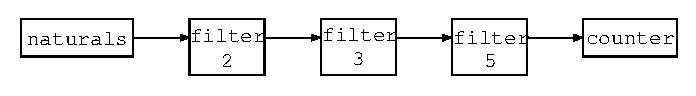
\includegraphics{fig/pipeline.eps}
\caption{}
\label{pipe_line}
\end{center}
\end{figure}

%\begin{program}
\begin{Verbatim}[baselinestretch=0.8]
        :- module main.

        main :- true|
            main(10000,Answer),
            io:outstream([print(Answer),nl]).

        main(Target,Answer) :- true|
            naturals(1,Target,Stream0),
            filter(2,Stream0,Stream1),
            filter(3,Stream1,Stream2),
            filter(5,Stream2,Stream3),
            counter(0,Stream3,Answer).

        naturals(N,M,List) :- N>=M |
            List=[].
        naturals(N,M,List) :- N<M  |
            List=[N|Rest],
            N1:=N+1,
            naturals(N1,M,Rest).

        filter(_,[],Out) :- true |
            Out = [].
        filter(X,[E|InN],Out) :- true |
            filter(X,E,InN,Out).

        filter(X,E,InN,Out) :- E mod X =:= 0 |
            EN := E / X,
            filter(X,EN,InN,Out).
        filter(X,E,InN,Out) :- E mod X =\= 0 |
            Out = [E|OutN],
            filter(X,InN,OutN).

        counter(C,[],Res) :- true |
            Res = C.
        counter(C,[1|InN],Res) :- true |
            CN := C + 1,
            counter(CN,InN,Res).
        counter(C,[E|InN],Res) :- E =\= 1 |
            counter(C,InN,Res).
\end{Verbatim}
%\end{program}

\verb!Target!=10000とした時の答えは,174である.  

\answer{データ記録方法の練習}
\begin{Verbatim}[baselinestretch=0.8]
  sort(I, O) :- true | sort(I, O,[]).

  sort([]   , C0,C) :- true | C0 = C.
  sort([H|T], C0,C) :- true | compare(T,H,[],[],L,R),
       sort(L, C0,C1), C1 = [H|C2], sort(R, C2,C).

  compare([]   ,V,L,R, OL,OR) :-   true   | OL = L, OR = R.
  compare([H|T],V,L,R, OL,OR) :-  H > V   | NL = [H|L], compare(T,V,NL,R, OL,OR).
  compare([H|T],V,L,R, OL,OR) :-  H =< V  | NR = [H|R], compare(T,V,L,NR, OL,OR).
\end{Verbatim}

LIFO法では,  データの終端をもらうまで次の分類に移れない.  また出力のための
引数を持ち回らなければならず,FIFO法より不利になる. 

\answer{ソートの練習}
\begin{Verbatim}[baselinestretch=0.8]
  :- module main.

  main :- data:sort(X), qsort(X).

  qsort(In) :- true | terminal(In,Out,[]), io:outstream(Out).

  node([]   ,V,N,L,R,Xs,Ys) :-  true   | L = [], R = [], Xs=[print(hist(V,N)),nl|Ys].
  node([H|T],V,N,L,R,Xs,Ys) :-  H < V  | L = [H|NL], node(T,V,N,NL,R,Xs,Ys).
  node([H|T],V,N,L,R,Xs,Ys) :-  H > V  | R = [H|NR], node(T,V,N,L,NR,Xs,Ys).
  node([H|T],V,N,L,R,Xs,Ys) :- H =:= V | M := N+1, node(T,V,M,L,R,Xs,Ys).

  terminal([]   ,Xs ,Ys) :- true | Xs = Ys.
  terminal([H|T],Xs0,Ys) :- true |
       terminal(L,Xs0,Xs1), node(T,H,1,L,R,Xs1,Xs2), terminal(R,Xs2,Ys).

実行結果:

  hist(0,8)
  hist(1,8)
  hist(2,12)
  hist(3,12)
  hist(4,10)
  hist(5,8)
  hist(6,9)
  hist(7,7)
  hist(8,12)
  hist(9,14)
\end{Verbatim}

\answer{2段ソートの練習}
\begin{Verbatim}[baselinestretch=0.8]
  :- module(main).

  main :- data:sort(X), qsort(X).

  qsort(In) :- true | term1(In,Mid,[]), term2(Mid,Out,[]), io:outstream(Out).

  node1([]   ,V,N,L,R,Xs,Ys) :-  true   | L = [], R = [], Xs=[(N-V)|Ys].
  node1([H|T],V,N,L,R,Xs,Ys) :-  H > V  | R = [H|NR], node1(T,V,N,L,NR,Xs,Ys).
  node1([H|T],V,N,L,R,Xs,Ys) :-  H < V  | L = [H|NL], node1(T,V,N,NL,R,Xs,Ys).
  node1([H|T],V,N,L,R,Xs,Ys) :- H =:= V | M := N+1, node1(T,V,M,L,R,Xs,Ys).

  term1([]   ,Xs ,Ys) :- true | Xs = Ys.
  term1([H|T],Xs0,Ys) :- true |
       term1(L,Xs0,Xs1), node1(T,H,1,L,R,Xs1,Xs2), term1(R,Xs2,Ys).

  node2([]       ,V,L,R) :-  true   | L = [], R = [].
  node2([(K-M)|T],V,L,R) :-  K =< V | R = [(K-M)|NR], node2(T,V,L,NR).
  node2([(K-M)|T],V,L,R) :-  K >  V | L = [(K-M)|NL], node2(T,V,NL,R).

  term2([]   ,Xs ,Ys) :- true | Xs = Ys.
  term2([(K-M)|T],Xs0,Ys) :- true |
       term2(L,Xs0,Xs1), Xs1 = [print(hist(M,K),nl|Xs2], 
       node2(T,K,L,R), term2(R,Xs2,Ys).

実行結果:

  hist(9,14)
  hist(2,12)
  hist(3,12)
  hist(8,12)
  hist(4,10)
  hist(6,9)
  hist(0,8)
  hist(1,8)
  hist(5,8)
  hist(7,7)
\end{Verbatim}

\answer{二進木の探索}

優先度制御により二進木を幅優先に探索するプログラムとその実行結果を以下
に示す.  また, このプログラムを実行した時のsearch/3のリダクションの様
子を図\ref{search_bf_log}に, 探索の様子を図\ref{search_tree2_bf}に示す.

\begin{quote}
\begin{Verbatim}[baselinestretch=0.8]
:- module main.                                                          % 1

main :- true |                                                           % 2
     ex:search_tree2(T), search(_,T,Ps), io:outstream([print(Ps),nl]).   % 3

search(abort,_,_) :- true | true.                                        % 4
alternatively.                                                           % 5
search(AB,n(L,R),Ps) :- true |                                           % 6
     cont(AB,LPs,RPs,ABL,ABR,Ps),                                        % 7
     search(ABL,L,LPs)@lower_priority, search(ABR,R,RPs)@lower_priority. % 8
search(_,Atom,Ps) :- atom(Atom) | Ps = [Atom].                           % 9
search(_,Int,Ps) :- integer(Int) | Ps = none.                            %10

cont(abort,_,_,ABL,ABR,_) :- true | ABL = abort, ABR = abort.            %11
alternatively.                                                           %12
cont(AB,LPs,_,_,ABR,Ps) :- list(LPs) | Ps = [left|LPs], ABR = abort.     %13
cont(AB,_,RPs,ABL,_,Ps) :- list(RPs) | Ps = [right|RPs], ABL = abort.    %14
cont(_,none,none,_,_,Ps) :- true | Ps = none.                            %15

%---------------------------------------------------------------------------

:- module ex.                                                            %16

search_tree2(T) :- T = n(n(n(n(1,n(2,3)),n(4,n(n(a,5),6))),n(b,7)),      %17
                         n(n(n(8,n(9,c)),10),n(n(d,11),12))).            %18
\end{Verbatim}
\end{quote}

\begin{Verbatim}[baselinestretch=0.8]
実行結果:
     [left,right,left,b]
\end{Verbatim}

\begin{figure}
\begin{center}
\begin{Verbatim}[baselinestretch=0.8]
 3 REDU:main:search(_B,n(n(n(n(..),n(..)),n(b,7)),                      %  1
                       n(n(n(..),10),n(n(..),12))),_3) :-               %  2
 7 REDU:main:search(_13,n(n(n(8,n(..)),10),n(n(d,11),12)),_63DF) :-     %  3
 6 REDU:main:search(_18,n(n(n(1,n(..)),n(4,n(..))),n(b,7)),_63E0) :-    %  4
13 REDU:main:search(_4A,n(b,7),_63BC) :-                                %  5
12 REDU:main:search(_4F,n(n(1,n(2,3)),n(4,n(n(..),6))),_63BD) :-        %  6
10 REDU:main:search(_30,n(n(d,11),12),_63CD) :-                         %  7
 9 REDU:main:search(_35,n(n(8,n(9,c)),10),_63CE) :-                     %  8
25 REDU:main:search(_B2,10,none) :-                                     %  9
24 REDU:main:search(_B7,n(8,n(9,c)),_6376) :-                           % 10
22 REDU:main:search(_98,12,none) :-                                     % 11
21 REDU:main:search(_9D,n(d,11),_6363) :-                               % 12
19 REDU:main:search(_7E,n(4,n(n(a,5),6)),_639A) :-                      % 13
18 REDU:main:search(_83,n(1,n(2,3)),_639B) :-                           % 14
16 REDU:main:search(_64,7,none) :-                                      % 15
15 REDU:main:search(_69,b,[b]) :-                                       % 16
39 REDU:main:search(abort,n(2,3),_6330)                                 % 17
38 REDU:main:search(abort,1,_6331)                                      % 18
36 REDU:main:search(abort,n(n(a,5),6),_6341)                            % 19
35 REDU:main:search(abort,4,_6342)                                      % 20
33 REDU:main:search(abort,11,_6352)                                     % 21
32 REDU:main:search(abort,d,_6353)                                      % 22
29 REDU:main:search(abort,n(9,c),_6365)                                 % 23
28 REDU:main:search(abort,8,_6366)                                      % 24
\end{Verbatim}
\caption{bf.kl1の実行トレース(search/3のリダクション)}
\label{search_bf_log}
\end{center}
\end{figure}

\begin{figure}
\begin{center}
% \epsfile{file=search_tree2_bf.eps}
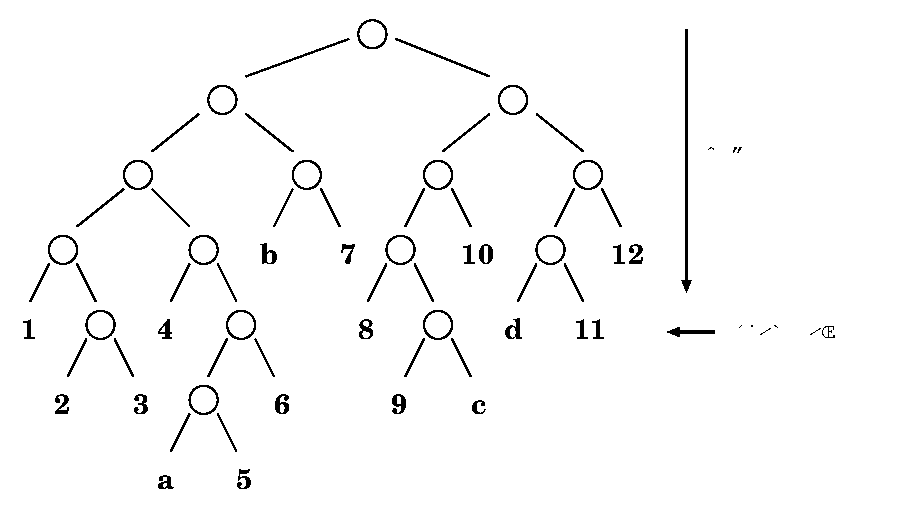
\includegraphics{fig/search_tree2_bf.eps}
\caption{bf.kl1実行におけるノードの探索}
\label{search_tree2_bf}
\end{center}
\end{figure}

\newpage
\answer{ストリームの要素を除去するプログラム}

\begin{Verbatim}[baselinestretch=0.8]
:- module main.

main :- true|
    data(List), remove(1,List,Out), io:outstream([print(Out),nl]).

remove(_,[],      Out) :- true   | Out=[].
remove(X,[X|List],Out) :- true   | remove(X,List,Out).
remove(X,[Y|List],Out) :- X \= Y | Out=[Y|OutN], remove(X,List,OutN).

data(List) :- true| List=[1,2,1,3,1].

% ``\='' の代わりに ``otherwise'' を用いると remove/3 は次のようになる.

remove(_,[],      Out) :- true   | Out=[].
remove(X,[X|List],Out) :- true   | remove(X,List,Out).
otherwise.
remove(X,[Y|List],Out) :- true   | Out=[Y|OutN], remove(X,List,OutN).
\end{Verbatim}

\verb|remove/3| は入力ストリームに対して部分的な透過性を持つフィルタで
ある. 第2引数の入力ストリームから第1引数の要素と同じものをすべて除いた
ストリームを第3引数に返す. 


\answer{ストリームを圧縮するプログラム}

\begin{Verbatim}[baselinestretch=0.8]
:- module main.

main :- true|
    data(List), compact(List,Out), io:outstream([print(Out),nl]).

compact([X|List],Out) :- true|
    Out=[X|OutN], remove(X,List,ListN), compact(ListN,OutN).
compact([],      Out) :- true| Out=[].

remove(_,[],      Out) :- true   | Out=[].
remove(X,[X|List],Out) :- true   | remove(X,List,Out).
remove(X,[Y|List],Out) :- X \= Y | Out=[Y|OutN], remove(X,List,OutN).

data(List) :- true| List=[1,2,3,4,5,4,3,2,1].
\end{Verbatim}

\verb|compact/2| は第1引数に圧縮すべき入力ストリームをとり, 結果を第2
引数に返す. \verb|compact/2| は要素が到着するのを待ち, 要素が来たらそ
れを出力ストリームに流し, その要素と同じものをそれ以降のストリームから
除去するプロセス(\verb|remove/3|)と, その結果を更に圧縮するプロセス
(\verb|compact/2|)とに分岐する.

\answer{1,000 以下の素数列を生成するプログラム}

\begin{Verbatim}[baselinestretch=0.8]
:- module main.                                                           %  1
main :- primes:primes(1000, C), io:outstream([print(C),nl]).              %  2

:- module primes.                                                         %  3
primes(Max,C) :- gen_primes(Max,Ps), count(Ps,C).                         %  4

% Max 以下の素数列を生成する.
gen_primes(Max,Ps) :- gen(2,Max,Ns), sift(Ns,Ps).                         %  5

% N0 〜 Max の自然数を生成する.  Ns0=[N0,N0+1,N0+2,...,Max]
gen(N0,Max,Ns0) :- N0=<Max | Ns0=[N0|Ns1], N1:=N0+1, gen(N1,Max,Ns1).     %  6
gen(N0,Max,Ns0) :- N0 >Max | Ns0=[].                                      %  7

% 新しい素数が入力ストリームより流れてきたならば, その素数を
% 用いたフィルタ・プロセスを生成する.  そして素数カウンタに
% 新しい素数を送る.
sift([],     Zs0) :- Zs0=[].                                              %  8
sift([P|Xs1],Zs0) :- Zs0=[P|Zs1], filter(P,Xs1,Ys), sift(Ys,Zs1).         %  9

% 入力 X が素数 P で割り切れない場合, 素数候補として X  を次の
% フィルタに送る.
filter(_,[],     Ys0) :-               Ys0=[].                            % 10
filter(P,[X|Xs1],Ys0) :- X mod P=\=0 | Ys0=[X|Ys1], filter(P,Xs1,Ys1).    % 11
filter(P,[X|Xs1],Ys0) :- X mod P=:=0 |              filter(P,Xs1,Ys0).    % 12

% 素数をカウントする.
count(L,C) :- count(L,0,C).                                               % 13

count([],C0,C) :- C=C0.                                                   % 14
count([_|T],C0,C) :- C1:=C0+1, count(T,C1,C).                             % 15

実行結果(個数の表示)
168
\end{Verbatim}

\newpage

\answer{20,000 以下の素数列を生成するプログラム}

要求駆動のプログラムと優先度制御を利用したプログラムを示す.  

\subsection*{要求駆動のプログラム}

\begin{Verbatim}[baselinestretch=0.8]
:- module main.                                                           %  1
main :- primes:primes(20000, 100, C), io:outstream([print(C),nl]).        %  2

:- module primes.                                                         %  3
% Sync: メッセージ next の流れるストリームとなる変数である.
% gen_primes はメッセージ next を最初の 1 回を除いて count から受け取る.
% Max以下 (Max1未満) の素数列を生成する. 
primes(Max,Unit,C) :- Max1:=Max+1,                                        %  4
        gen_primes(Max1,Unit,Ps,[next|Sync]), count(Ps,C,Sync).           %  5

% Max 未満の素数列を生成する.
gen_primes(Max,Unit,Ps,Sync) :- gen(Sync,2,Max,Unit,Ns), sift(Ns,Ps).     %  6

% 2 以上の自然数を Unit個ずつ生成する.
% 自然数列の区切り記号として 1 を利用する.
gen([next|_],   N0,Max,Unit,Ns0) :- N1:=N0+Unit, Max=<N1 |                %  7
        gen_unit(N0,Max,Ns0,[]).                                          %  8
gen([next|Sync],N0,Max,Unit,Ns0) :- N1:=N0+Unit, Max >N1 |                %  9
        gen_unit(N0,N1,Ns0,[1|Ns]), gen(Sync,N1,Max,Unit,Ns).             % 10

% N0 〜 Max-1 の自然数を生成する.  Ns0=[N0,N0+1,N0+2,...,Max-1|Ns]
gen_unit(N0,Max,Ns0,Ns) :- N0< Max |                                      % 11
        Ns0=[N0|Ns1], N1:=N0+1, gen_unit(N1,Max,Ns1,Ns).                  % 12
gen_unit(N0,Max,Ns0,Ns) :- N0>=Max | Ns0=Ns.                              % 13

% 新しい素数が入力ストリームより流れてきたならば, その素数を
% 用いたフィルタ・プロセスを生成する.  そして素数カウンタに
% 新しい素数を送る.
% 素数 P として 1 が来た場合は, 区切り記号が到着したことを
% 意味するので 次の自然数列の発生を要求するためにメッセージ
% next を送る.
sift([],     Zs0) :- Zs0=[].                                              % 14
sift([P|Xs1],Zs0) :- P=\=1 |Zs0=[P|Zs1], filter(P,Xs1,Ys), sift(Ys,Zs1).  % 15
sift([1|Xs1],Zs0) :- Zs0=[1|Zs1], sift(Xs1,Zs1).                          % 16

% 入力 X が素数 P で割り切れない場合, 素数候補として X  を次の
% フィルタに送る.
filter(_,[],     Ys0) :-               Ys0=[].                            % 17
filter(P,[X|Xs1],Ys0) :- X mod P=\=0 | Ys0=[X|Ys1], filter(P,Xs1,Ys1).    % 18
filter(P,[X|Xs1],Ys0) :- X mod P=:=0 |              filter(P,Xs1,Ys0).    % 19

% 素数をカウントする. 1 を受け取った場合は, 次の自然数列の発生を
% 促すためにメッセージ send を Sync に送る.
count(L,C,Sync) :- count(L,0,C,Sync).                                     % 20

count([],C0,C,_) :- C=C0.                                                 % 21
count([P|T],C0,C,Sync) :- P =\= 1 | C1:=C0+1, count(T,C1,C,Sync).         % 22
count([1|T],C0,C,Sync) :- Sync=[next|Sync1], count(T,C0,C,Sync1).         % 23

実行結果(個数の表示)
2262
\end{Verbatim}

\subsection*{優先度を利用したプログラム}

\begin{Verbatim}[baselinestretch=0.8]
:- module main.                                                           %  1
main :- primes(20000,NP), io:outstream([print(NP),nl]).                   %  2

primes(Max,NP) :- gen_primes(Max,Ps), count(Ps,NP).                       %  3

gen_primes(Max,Ps) :- gen(2,Max,Ns)@lower_priority, sift(Ns,Ps).          %  4

gen(N,Max,Ns) :- N >Max | Ns=[].                                          %  5
gen(N,Max,Ns) :- N=<Max | Ns=[N|Ns2], N2:=N+1, gen(N2,Max,Ns2).           %  6

sift([],    Zs) :- Zs=[].                                                 %  7
sift([P|Xs],Zs) :- Zs=[P|Zs2], filter(P,Xs,Ys), sift(Ys,Zs2).             %  8

filter(_,[],    Ys) :-               Ys=[].                               %  9
filter(P,[X|Xs],Ys) :- X mod P=\=0 | Ys=[X|Ys2], filter(P,Xs,Ys2).        % 10
filter(P,[X|Xs],Ys) :- X mod P=:=0 |             filter(P,Xs,Ys).         % 11

count(Ps,NP) :- count(Ps,0,NP).                                           % 12

count([],    WNP,NP) :- WNP=NP.                                           % 13
count([P|Ps],WNP,NP) :- WNP2:=WNP+1, count(Ps,WNP2,NP).                   % 14

実行結果(個数の表示)
2262
\end{Verbatim}

\newpage

\answer{1,000 番目の素数を求めるプログラム}

\begin{Verbatim}[baselinestretch=0.8]
:- module main.                                                           %  1
main :- primes(1000,LP), io:outstream([print(LP),nl]).                    %  2

primes(Nth,LP) :- gen_primes(AB,Ps), pkup(Ps,Nth,AB,LP).                  %  3

gen_primes(AB,Ps) :- gen(AB,2,Ns)@lower_priority, sift(Ns,Ps).            %  4

gen(abort,_,Ns) :- Ns=[].                                                 %  5
alternatively.                                                            %  6
gen(AB,   N,Ns) :- Ns=[N|Ns2], N2:=N+1, gen(AB,N2,Ns2).                   %  7

sift([],    Zs) :- Zs=[].                                                 %  8
sift([P|Xs],Zs) :- Zs=[P|Zs2], filter(P,Xs,Ys), sift(Ys,Zs2).             %  9

filter(_,[],    Ys) :-               Ys=[].                               % 10
filter(P,[X|Xs],Ys) :- X mod P=\=0 | Ys=[X|Ys2], filter(P,Xs,Ys2).        % 11
filter(P,[X|Xs],Ys) :- X mod P=:=0 |             filter(P,Xs,Ys).         % 12

pkup([P|_], Nth,AB,LP) :- Nth=:=1 | LP=P, AB=abort.                       % 13
pkup([_|Ps],Nth,AB,LP) :- Nth=\=1 | Nth2:=Nth-1, pkup(Ps,Nth2,AB,LP).     % 14

実行結果(1000個目の素数の表示)
7919
\end{Verbatim}

\begin{thebibliography}{1}

\bibitem{PIMOS}
Takashi Chikayama, Hiroyuki Sato, and Toshihiko Miyazaki.
\newblock Overview of the parallel inference machine operating system
  ({P}{I}{M}{O}{S}).
\newblock In {\em Proceedings of FGCS'88}, pages 230--251, Tokyo, Japan, 1988.

\bibitem{parlog}
Keith~L. Clark and Steve Gregory.
\newblock Parlog: A parallel logic programming language.
\newblock {\em ACM Transaction on Programming Languages and Systems}, 8(1),
  1986.

\bibitem{CP}
Ehud Shapiro.
\newblock A subset of {C}oncurrent {P}rolog and its interpreter.
\newblock ICOT Technical Report TR-003, ICOT, 1983.

\bibitem{OOCP}
Ehud Shapiro and Akikazu Takeuchi.
\newblock Object oriented programming in {C}oncurrent {P}rolog.
\newblock ICOT Technical Report TR-004, ICOT, 1983.
\newblock Also in New Generation Computing, Springer-Verlag Vol.1 No.1,1983.

\bibitem{GHCoriginal}
Kazunori Ueda.
\newblock {G}uarded {H}orn {C}lauses.
\newblock ICOT Technical Report TR-103, ICOT, 1985.

\bibitem{KL-Design}
Kazunori Ueda and Takashi Chikayama.
\newblock Design of the kernel language for the parallel inference machine.
\newblock {\em The Computer Journal}, December 1990.

\bibitem{KLIC} 
Takashi Chikayama, Tetsuro Fujise and Daigo Sekita.
\newblock A Portable and Efficient Implementation of KL1.
\newblock {\em Proceedings of PRILP'94}, Lecture Notes in Computer Science
\#884, Springer-Verlag, 1994.
\end{thebibliography}

\end{document}
